%\documentclass[acmsmall,review]{acmart}
\documentclass[acmsmall, screen]{acmart}
%\settopmatter{printfolios=true,printccs=false,printacmref=false}

\startPage{1}

\bibliographystyle{ACM-Reference-Format}
\citestyle{acmauthoryear}   %% For author/year citations

\usepackage{booktabs}   %% For formal tables:
                        %% http://ctan.org/pkg/booktabs
\usepackage{subcaption} %% For complex figures with subfigures/subcaptions
                        %% http://ctan.org/pkg/subcaption

\usepackage{algorithm}% http://ctan.org/pkg/algorithms
\usepackage{algpseudocode}% http://ctan.org/pkg/algorithmicx

\usepackage{boldline,multirow}

\usepackage{makecell, multirow}
\usepackage[inline]{enumitem}
\usepackage{listings}
\usepackage{graphicx}
\usepackage{color}

\usepackage{tabulary} \usepackage{tabularx}

\usepackage{tikz} \usetikzlibrary{shapes,arrows,positioning}
\usepackage{multicol}

\usepackage{proof}

\usepackage{caption}
% \usepackage{subcaption}
\definecolor{dkgreen}{rgb}{0,0.6,0}
\definecolor{gray}{rgb}{0.5,0.5,0.5}
\definecolor{mauve}{rgb}{0.58,0,0.82}

\lstset{ language=Java, aboveskip=3mm, belowskip=3mm,
  showstringspaces=false, columns=flexible,
  basicstyle={\small\ttfamily}, numbers=left, numbersep=5pt,
  numberstyle=\small\color{gray}, keywordstyle=\color{blue},
  commentstyle=\color{dkgreen}, stringstyle=\color{mauve},
  breaklines=true, breakatwhitespace=true, tabsize=3 }

% \tikzstyle{block} = [rectangle, draw, fill=white, text width=5em,
% text centered, rounded corners, minimum height=4em]
\tikzstyle{block} = [rectangle, draw, fill=white, text width=3em, text
centered, rounded corners, minimum height=3em] 
\tikzstyle{block2} =
[rectangle, draw, fill=white, text width=5em, text centered, rounded
corners, minimum height=3em] \tikzstyle{line} = [draw, -latex']
\setcopyright{rightsretained}





\begin{document}

% %% Title information
% \title[Short Title]{Full Title} %% [Short Title] is optional;
%                                         %% when present, will be
%                                         %% used in
%                                         %% header instead of Full
%                                         %% Title.
% \titlenote{with title note} %% \titlenote is optional;
%                                         %% can be repeated if
%                                         %% necessary;
%                                         %% contents suppressed with
%                                         %% 'anonymous'
% \subtitle{Subtitle} %% \subtitle is optional
% \subtitlenote{with subtitle note} %% \subtitlenote is optional;
%                                         %% can be repeated if
%                                         %% necessary;
%                                         %% contents suppressed with
%                                         %% 'anonymous'


% \title{Context Tunneling for Points-to Analysis}
% \subtitle{Maximizing the Potential of $k$-Context-Sensitivity with
% Data-Driven Optimization}
\title{Precise and Scalable Points-to Analysis via Data-Driven Context
  Tunneling}

\author{Minseok Jeon}
\email{minseok_jeon@korea.ac.kr} %% \email is recommended
\affiliation{
	% \position{Student}
	\department{Department of Computer Science and
		Engineering} %% \department is recommended
	\institution{Korea University} %% \institution is required
	\streetaddress{145, Anam-ro} \city{Sungbuk-gu} \state{Seoul}
	\postcode{02841} \country{Republic of Korea} }
\author{Sehun Jeong} \email{gifaranga@korea.ac.kr}
\affiliation{
	% \position{Student}
	\department{Department of Computer Science and
		Engineering} %% \department is recommended
	\institution{Korea University} %% \institution is required
	\streetaddress{145, Anam-ro} \city{Sungbuk-gu} \state{Seoul}
	\postcode{02841} \country{Republic of Korea} }
\author{Hakjoo Oh}
\authornote{Corresponding author}
\email{hakjoo_oh@korea.ac.kr} %% \email is recommended
\affiliation{
  % \position{Student}
  \department{Department of Computer Science and
    Engineering} %% \department is recommended
  \institution{Korea University} %% \institution is required
  \streetaddress{145, Anam-ro} \city{Sungbuk-gu} \state{Seoul}
  \postcode{02841} \country{Republic of Korea} }


\begin{CCSXML}
	<ccs2012>
	<concept>
	<concept_id>10003752.10010124.10010138.10010143</concept_id>
	<concept_desc>Theory of computation~Program analysis</concept_desc>
	<concept_significance>500</concept_significance>
	</concept>
	<concept>
	<concept_id>10010147.10010257.10010293</concept_id>
	<concept_desc>Computing methodologies~Machine learning approaches</concept_desc>
	<concept_significance>500</concept_significance>
	</concept>
	</ccs2012>
\end{CCSXML}

\ccsdesc[500]{Theory of computation~Program analysis}
\ccsdesc[500]{Computing methodologies~Machine learning approaches}

%%% The following is specific to OOPSLA '18 and the paper
%%% 'Precise and Scalable Points-to Analysis via Data-Driven Context Tunneling'
%%% by Minseok Jeon, Sehun Jeong, and Hakjoo Oh.
%%%
\acmPrice{}
\acmDOI{10.1145/3276510}
\acmYear{2018}
\copyrightyear{2018}
\acmJournal{PACMPL}
\acmVolume{2}
\acmNumber{OOPSLA}
\acmArticle{140}
\acmMonth{11}


%% Keywords comma separated list
\keywords{Points-to analysis, Context-sensitive analysis, Data-driven
  program
  analysis} %% \keywords are mandatory in final camera-ready submission

\newcommand{\mca}{\mathcal{A}}
\newcommand{\mcb}{\mathcal{B}}
\newcommand{\mcc}{\mathcal{C}}
\newcommand{\mcf}{\mathcal{F}}
\newcommand{\mcg}{\mathcal{G}}
\newcommand{\mcp}{\mathcal{P}}
\newcommand{\mcl}{\mathcal{L}}
\newcommand{\mcm}{\mathcal{M}}
\newcommand{\mco}{\mathcal{O}}
\newcommand{\mcu}{\mathcal{U}}
\newcommand{\mcv}{\mathcal{V}}
\newcommand{\mcr}{\mathcal{R}}

\newcommand{\myland}{\;\land\;}
\newcommand{\mylor}{\;\vee\;}

\newcommand{\power}[1]{\wp(#1)}

\newcommand{\myset}[1]{\{ #1 \}}
\newcommand{\myvec}[1]{\langle #1 \rangle}

\newcommand{\db}[1]{\llbracket #1 \rrbracket}
\newcommand{\pdb}[1]{\llbracket #1 \rrbracket_{\pconf}}
\newcommand{\ppdb}[1]{\llbracket #1 \rrbracket^{\pre}}
\newcommand{\po}{{po}}




%%%%Tunneling


%% Learning
\newcommand{\Classifier}{\mathcal{C}}
%\newcommand{\argmax}[1]{\underset{#1}{\mathrm{argmax}}}
\newcommand{\argmax}{\operatornamewithlimits{argmax}}

%% Comment
\newcommand{\todoc}[2]{{\textcolor{#1} {\textbf{[[#2]]}}}}

\newcommand{\todored}[1]{\todoc{red}{#1}}
\newcommand{\todoblue}[1]{\todoc{blue}{#1}}
\newcommand{\todogreen}[1]{\todoc{green}{#1}}

\newcommand*{\TODO}[1]{\todored{#1}}
\newcommand*{\minseok}[1]{\todoblue{Minseok: #1}}
\newcommand{\commentout}[1]{}

\newcommand{\abst}{}
\newcommand{\aF}{\abst{F}}
\newcommand{\oracle}{{\mathcal{O}}}
\newcommand{\floor}[1]{\lfloor #1 \rfloor}
%% Program
\newcommand{\mba}{\mathbb{A}}
\newcommand{\mbb}{\mathbb{B}}
\newcommand{\mbc}{\mathbb{C}}
\newcommand{\mbd}{\mathbb{D}}
\newcommand{\mbe}{\mathbb{E}}
\newcommand{\mbf}{\mathbb{F}}
\newcommand{\mbg}{\mathbb{G}}
\newcommand{\mbh}{\mathbb{H}}
\newcommand{\mbi}{\mathbb{I}}
\newcommand{\mbj}{\mathbb{J}}
\newcommand{\mbk}{\mathbb{K}}
\newcommand{\mbl}{\mathbb{L}}
\newcommand{\mbm}{\mathbb{M}}
\newcommand{\mbn}{\mathbb{N}}
\newcommand{\mbo}{\mathbb{O}}
\newcommand{\mbp}{\mathbb{P}}
\newcommand{\mbq}{\mathbb{Q}}
\newcommand{\mbr}{\mathbb{R}}
\newcommand{\mbs}{\mathbb{S}}
\newcommand{\mbt}{\mathbb{T}}
\newcommand{\mbu}{\mathbb{U}}
\newcommand{\mbv}{\mathbb{V}}
\newcommand{\mbw}{\mathbb{W}}
\newcommand{\mbx}{\mathbb{X}}
\newcommand{\mby}{\mathbb{Y}}
\newcommand{\mbz}{\mathbb{Z}}
\newcommand{\cfgto}{\hookrightarrow}

\newcommand*{\cD}{\mathcal{D}}
\newcommand*{\cF}{\mathcal{F}}
\newcommand*{\cP}{\mathcal{P}}
\newcommand*{\cV}{\mathcal{V}}

\newcommand{\mcs}{\mathcal{S}}
\newcommand{\wv}{\mathbf{w}}
\newcommand{\Pgm}{{\it Pgm}}

\newcommand{\Hint}{{\it Profile}}
\newcommand{\hint}{R}
\newcommand{\compo}{\mbj}
\newcommand{\importance}{\mbr}
\newcommand{\feat}{f}
\newcommand{\features}{{\vec{\feat}}}
\newcommand{\strategy}{\mathcal{S}}

\newcommand{\score}{{\it score}}

\newcommand{\mse}{E}

\let\oldvec\vec
\renewcommand{\vec}[1]{\mathbf{#1}}


\newcommand{\obj}{{\it obj}}
\newcommand{\model}{\mathcal{M}}
\newcommand{\counter}{\mathcal{C}}
\newcommand{\lfp}{{\sf lfp}}
\newcommand{\widenop}{\triangledown}
\newcommand{\lub}{{\it lub}}
\newcommand{\glb}{{\it glb}}

\newcommand*{\sans}{\fontfamily{phv}\selectfont}
\newcommand*{\cour}{\fontfamily{pcr}\selectfont}

\newcommand{\true}{{\it true}}
\newcommand{\false}{{\it false}}
\newcommand{\afeatures}{\mba}
\newcommand{\afeat}{a}
\newcommand{\Methods}{{\mbm}}
\newcommand{\Invos}{{\mbi}}
\newcommand{\sem}[1]{[\![#1]\!]}
\newcommand{\mthd}{{{M}}}
\newcommand{\Program}{\mbp}
\newcommand{\selector}{S}
\newcommand{\component}{\mbm}
\newcommand{\idx}{j}
\newcommand{\heuristic}{\mathcal{H}}
\newcommand{\weight}{\vec{w}}
\newcommand{\formulas}{\mcf}
\newcommand{\cost}{{\sf cost}}
\newcommand{\proved}{{\sf proved}}
\newcommand{\method}{{\sf meth}}
\newcommand{\precision}{\proved}

\newcommand{\pr}{\Psi}

\newcommand{\Assertion}{\mbq}

\newcommand{\params}{\Pi}
\newcommand{\lparams}{\Theta}
\newcommand{\lparam}{\theta}

\renewcommand{\algorithmicrequire}{\textbf{Input:}}
\renewcommand{\algorithmicensure}{\textbf{Output:}}
\newcommand{\ChooseClause}{{\sf ChooseClause}}
\newcommand{\ChooseAtom}{{\sf ChooseRefiner}}
\newcommand{\ChooseSeed}{{\sf ChooseSeed}}
\newcommand{\RefineSeed}{{\textsc{RefineSeed}}}
\newcommand{\PrecP}{{\sf Prec^{+}}}
\newcommand{\PrecE}{{\sf Prec^{=}}}
\newcommand{\CostM}{{\sf Cost^{-}}}
\newcommand{\HasSeed}{{\sf HasPotential}}
\newcommand{\GoodHeuristicFound}{{\sf BetterHeuristicFound}}
\newcommand{\isSatisfactory}{{\sf isSatisfactoryPrecision}}

\newcommand{\hypospace}{\mathcal{M}}

\newcommand{\AnalyzeWith}{{\sf Analyze}}

\newcommand{\Record}{{\sf record}}
\newcommand{\Merge}{{\sf merge}}
\newcommand{\MergeTunneled}{\textbf{\textsc{ParentContext}}}
\newcommand{\MergeStatic}{\textbf{\textsc{MergeStatic}}}
\newcommand{\ectx}{\star}
\newcommand{\ApplyDepth}{\textsc{\textbf{ApplyDepth}}}
\newcommand{\Tunnel}{\textsc{\textbf{Tunnel}}}
\newcommand{\ContextMadeIn}{{{\textsc{\textbf{ParentMethod}}}}}
\newcommand{\Tunneling}{{{\textsc{{Tunneling}}}}}
\newcommand{\TunnelingRelation}{\mathcal{T}}

\newcommand{\childMeth}{{\it childMeth}}

\newcommand{\onesobjH}{{\it S1objH}}
\newcommand{\oneobjH}{{\it 1objH}}
\newcommand{\onetypeH}{{\it 1typeH}}
\newcommand{\onecallH}{{\it 1callH}}
\newcommand{\onecall}{{\it 1call}}

\newcommand{\onesobjHT}{{\it S1objH+T}}
\newcommand{\bonesobjHT}{{\textit{\textbf{S1objH+T}}}}
\newcommand{\oneobjHT}{{\it 1objH+T}}
\newcommand{\onetypeHT}{{\it 1typeH+T}}
\newcommand{\onecallHT}{{\it 1callH+T}}

\newcommand{\twosobjH}{{\it S2objH}}
\newcommand{\threesobjH}{{\it S3obj2H}}
\newcommand{\twoobjH}{{\it 2objH}}
\newcommand{\twotypeH}{{\it 2typeH}}
\newcommand{\twocallH}{{\it 2callH}}

\newcommand{\kobjkH}{{\it kobj+kH}}

\newcommand{\sobjHdata}{{\it \sobjH+Data}}
\newcommand{\objHdata}{{\it \objH+Data}}
\newcommand{\typeHdata}{{\it \typeH+Data}}
\newcommand{\calldata}{{\it \call+Data}}

\newcommand{\sobjHIntroA}{{\it \sobjH+IntroA}}
\newcommand{\objHIntroA}{{\it \objH+IntroA}}
\newcommand{\typeHIntroA}{{\it \typeH+IntroA}}
\newcommand{\callHIntroA}{{\it \call+IntroA}}

\newcommand{\sobjHIntroB}{{\it \sobjH+IntroB}}
\newcommand{\objHIntroB}{{\it \objH+IntroB}}
\newcommand{\typeHIntroB}{{\it \typeH+IntroB}}
\newcommand{\callHIntroB}{{\it \call+IntroB}}

\newcommand{\pair}{{\it pair}}
\newcommand{\first}{{\it first}}
\newcommand{\second}{{\it second}}

\newcommand{\classof}{{\it classof}}
\newcommand{\methof}{{\it methof}}
\newcommand{\typeof}{{\it typeof}}
\newcommand{\lookup}{{\it lookup}}
%\newcommand{\methofinvo}{{\sf methof}}

\newcommand{\truncateCtx}[2]{{\lceil #1 \rceil_{#2}}}
%\newcommand{\truncateCtx}[2]{{\sf last}_{#2}(#1)}
\newcommand{\appendCtx}[2]{#1 \concat #2}

\newcommand{\ctxElem}{{\sf ctxof}}
\newcommand{\pctx}{{\it pctx}}
\newcommand{\parentCtx}{{\sf pctx}}
\newcommand{\parentMeth}{{\sf pmeth}}

\newcommand{\parentMethod}{{\sf pmeth}}

\newcommand{\hide}[1]{}

%%%%%%%%%%%%%%%%%%%%%%%%%%%%%%
%% relations for representing programs
%%%%%%%%%%%%%%%%%%%%%%%%%%%%%%

\newcommand{\meth}{{\it meth}}
\newcommand{\toMeth}{{\it m'}}
\newcommand{\inMeth}{{\it m}}

\newcommand{\ctx}{{\it ctx}}
\newcommand{\toCtx}{{\it c}_2}
\newcommand{\fromCtx}{{\it c}_1}
\newcommand{\hctx}{{\it hctx}}
\newcommand{\heap}{{\it heap}}
\newcommand{\var}{{\it x}}
\newcommand{\tovar}{{\it x}}
\newcommand{\fromvar}{{\it y}}
\newcommand{\base}{{\it z}}
\newcommand{\baseH}{{\it h}'}
\newcommand{\baseHCtx}{{\it hc}'}
\newcommand{\fld}{{\it f}}
\newcommand{\calleeCtx}{{\it c}_2}
\newcommand{\callerCtx}{{\it c}_1}
\newcommand{\invo}{{\it l}}

\newcommand{\this}{{\it this}}
\newcommand{\sig}{{\it sig}}
\newcommand{\heapT}{{\it hT}}

\newcommand{\Alloc}{\textsc{Alloc}}
\newcommand{\Move}{\textsc{Move}}
\newcommand{\Load}{\textsc{Load}}
\newcommand{\Store}{\textsc{Store}}
\newcommand{\VCall}{\textsc{Call}}
\newcommand{\SCall}{\textsc{SCall}}
\newcommand{\FormalArg}{\textsc{FormalArg}}
\newcommand{\ActualArg}{\textsc{ActualArg}}
\newcommand{\FormalReturn}{\textsc{FormalReturn}}
\newcommand{\ActualReturn}{\textsc{ActualReturn}}
\newcommand{\ThisVar}{\textsc{ThisVar}}
\newcommand{\HeapType}{\textsc{HeapType}}
\newcommand{\LookUp}{\textsc{LookUp}}

\newcommand{\VarPointsTo}{\textit{ptsto}}
\newcommand{\CallGraph}{\textit{callgraph}}
\newcommand{\FldPointsTo}{\textit{fldptsto}}
\newcommand{\InterProcAssign}{\textit{InterProcAssign}}
\newcommand{\Reachable}{\textit{reachable}}

\newcommand{\Flavor}{{\it flavor}}
\newcommand{\Flavorcall}{\Flavor_{\it call}}
\newcommand{\Flavorobj}{\Flavor_{\it obj}}
\newcommand{\Flavorsobj}{\Flavor_{\it sobj}}
\newcommand{\Flavortype}{\Flavor_{\it type}}

\newcommand{\parent}{\Flavor}
\newcommand{\parentcall}{\Flavorcall}
\newcommand{\parentsobj}{\Flavorsobj}
\newcommand{\parentobj}{\Flavorobj}
\newcommand{\parenttype}{\Flavortype}


\newcommand{\HeapDepth}{{\it maxH}}
\newcommand{\CallDepth}{{\it maxK}}


\newcommand{\concat}{%
  \mathbin{{+}\mspace{-8mu}{+}}%
}

\newcommand{\cmd}{{\it inst}}
\newcommand{\lcmd}{{\it linst}}

\newcommand{\Context}{\mbc}
\newcommand{\HeapContext}{\mbh\mbc}

\newcommand{\myparagraph}[1]{\paragraph{\fontshape{\itdefault}\fontseries{\bfdefault}\selectfont
#1\/}}

\newcommand{\Bean}{\textsc{Bean}}

\newcommand{\fprime}{f_{\it imp}}
\newcommand{\fsecond}{f_{\it unimp}}

\newcommand{\tspace}{\mcr}

\newcommand{\LearnBooleanFormula}{\textsc{LearnParameter}}
\newcommand{\CollectSeedFeatures}{\textsf{CollectSeedFeatures}}
\newcommand{\Failed}{{\it Failed}}

\newcommand{\SeedFeature}{\textsf{SeedFeature}}



%%Obj2CFA



\let\oldvec\vec
\renewcommand{\vec}[1]{\mathbf{#1}}




\renewcommand{\algorithmicrequire}{\textbf{Input:}}
\renewcommand{\algorithmicensure}{\textbf{Output:}}
\newcommand{\Update}{{\sf Update}}
\newcommand{\Prec}{{\sf Prec}}
\newcommand{\Refiner}{\Gamma}

\newcommand{\RefineClause}{{\sf RefineClause}}

\newcommand{\BetterThan}{{\sf Improved}}

\newcommand{\oneobjHTnew}{\oneobjHT$_{\it new}$}
%\newcommand{\oneobjHT}{{\it 1objH+$\objheuristic$}}

%\newcommand{\onecallHT}{{\it 1callH+$\callheuristic$}}

\newcommand{\callH}{{\it 1callH+S}}
%\newcommand{\bsimonecallH}{\textit{\textbf{1callH+S}}}
\newcommand{\sobjSimLearn}{{\it 1callH+SL'}}
\newcommand{\simonecallH}{{\it 1callH+S'}}

\newcommand{\kth}{\text{\it last}}

\newcommand{\Graphick}{{\sc Graphick}}
\newcommand{\Scaler}{{\it Scaler}}
\newcommand{\Zipper}{{\it Zipper}}
\newcommand{\twoobjZipper}{{\it 2objH+Zip}}
\newcommand{\oursZipper}{{\it 1callH+SL+Zip}}
%\newcommand{\Zipper}{{\it Zipper}}


\newcommand{\twoobjHT}{{\it 2objH+T}}
\newcommand{\ours}{{\it 1callH+SL}}
\newcommand{\oursim}{{\it 1callH+S}}
\newcommand{\oursbf}{{\it\textbf{1callH+SL}}}
%\newcommand{\ours}{{\it 1callH+$\heuristic_{\sf ours}$}}

\newcommand{\onecallThis}{{\it 1callH+T$_{C1}$}}

\newcommand{\onecallHours}{{\it 1callH+}$\heuristic_f$}
\newcommand{\onecallHdtree}{{\it 1callH+}$\heuristic$}
%\newcommand{\onecallHDT}{{\it 1callH+}$\heuristic_\decisionTree$}
\newcommand{\onecallHDT}{{\it 1callH+D}}
\newcommand{\onecallHL}{{\it 1callH+L}}


\newcommand{\threeobjH}{{\it 3obj2H}}


%%%%%%%%%%%%%%%%%%%%%%%%%%%%%%
%% relations for representing programs
%%%%%%%%%%%%%%%%%%%%%%%%%%%%%%




%\newcommand{\myparagraph}[1]{\paragraph{\fontshape{\itdefault}\fontseries{\bfdefault}\selectfont
%#1\/}}

\newcommand{\mybf}[1]{{\fontshape{\itdefault}\fontseries{\bfdefault}\selectfont#1\/}}



%\newcommand{\Simulation}{\textsc{Simulation}}
%\newcommand{\Recovery}{\textsc{Recovery}}


\newcommand{\CallGraphEdge}{{\sf CallGraphEdge}}


\newcommand{\Inst}{\text{\it Label}}
\newcommand{\Invo}{\text{\it Invo}}
\newcommand{\inst}{l}
\newcommand{\fix}{{\it fix}}
\newcommand{\entry}{\text{\it main}}
\newcommand{\emptyctx}{\epsilon}
\newcommand{\updatectx}{U}
\newcommand{\Var}{\text{\it Var}}
\newcommand{\Ctx}{\text{\it Ctx}}
\newcommand{\Heap}{\text{\it Heap}}
\newcommand{\Hctx}{\text{\it Hctx}}
\newcommand{\project}{\Pi}
\newcommand{\weakupdate}{\stackrel {{\it w}}{\mapsto}}


%\newcommand{\fld}{{\it fld}}
\newcommand{\ptsto}{X}
\newcommand{\fptsto}{Y}
\newcommand{\reachable}{R}
\newcommand{\callgraph}{G}

\newcommand{\mthdof}{\text{\it Mthdof}}

\newcommand{\moreprecise}{\succeq}
\newcommand{\strictlylessprecise}{\prec}


\newcommand{\decisionTree}{{\sf DT}}
\newcommand{\simulate}{{\sf simulate}}
\newcommand{\Tobj}{T_{\text{\it obj}}}
\newcommand{\call}{{\sf call}}
\newcommand{\Tcall}{T_{\text{\it call}}}
\newcommand{\learn}{{\sf learn}}
\newcommand{\callheuristic}{\heuristic_{\sf call}}
\newcommand{\objheuristic}{\heuristic_{\sf obj}}
\newcommand{\simheuristic}{\heuristic_{{\sf sim}}}
\newcommand{\dtheuristic}{\heuristic_{{\sf \decisionTree}}}
\newcommand{\ourheuristic}{\heuristic_{{\sf ours}}}



\newcommand{\featmean}[2]{\sem{#1}_{#2}}
\newcommand{\xor}{\oplus}

%\newcommand{\Gobj}{G_{\it obj}}
\newcommand{\Gobj}{G}
\newcommand{\transform}{{\sf transform}}

\newcommand{\objective}{{\it O}}


\newcommand{\learnold}{A}
\newcommand{\learnsup}{B}

\newcommand{\ourtechnique}{\textsc{Obj2Cfa}}



%\newcommand{\Existing}{{\it Existing}~\cite{JeJeOh18}}
\newcommand{\Existing}{{\it 1callH+T$_{\it new}$}}
\newcommand{\DecisionTree}{{\it Decision tree}}
\newcommand{\OurLearn}{{\it 1callH+SL}}

\newcommand{\failcasts}{\#may-fail-casts}

\newcommand{\callgraphedges}{\#call-graph-edges}
\newcommand{\reachableMethods}{\#reachable-methods}
\newcommand{\polycalls}{\#polymorphic-calls}



\newcommand{\ideal}{{\it ideal}}
\newcommand{\onepgm}{{\{luindex\}}}
\newcommand{\twopgm}{{\{luindex, lusearch\}}}
\newcommand{\threepgm}{{\{luindex, lusearch, antlr\}}}
\newcommand{\fourpgm}{{\{luindex, lusearch, antlr, pmd\}}}

\newcommand{\hyper}{{\theta}}

\newcommand{\Lait}{{\sc Lait}}
\newcommand{\Eagle}{\textsc{Eagle}}

\newcommand{\abs}{{\bf a}}
\newcommand{\absk}{{\bf k}}
\newcommand{\absz}{{\bf 0}}



\newcommand{\Refine}{{\textit{Refine}}}
\newcommand{\Specify}{{\textit{Specify}}}
\newcommand{\Score}{{\textit{Score}}}

\newcommand{\GraphPtsTo}{{{G_{\textit {FPG}}}}}
\newcommand{\NodePtsTo}{{{N_{\textit{FPG}}}}}
\newcommand{\EdgePtsTo}{{{\hookrightarrow_{\textit{FPG}}}}}

\newcommand{\GraphOAG}{{{G_{\textit{OAG}}}}}
\newcommand{\NodeOAG}{{{N_{\textit{OAG}}}}}
\newcommand{\EdgeOAG}{{{\hookrightarrow_{\textit{OAG}}}}}

\newcommand{\New}{{\textit{New}}}
\newcommand{\Replace}{{\textit{Replace}}}
\newcommand{\Append}{{\textit{Append}}}

\newcommand{\MaxIn}{{\textit{MaxIn}}}
\newcommand{\MaxOut}{{\textit{MaxOut}}}

\newcommand{\ourtool}{{\sc Graphick}}

\newcommand{\TypeBased}{{\it Type-Based}}
\newcommand{\AllocBased}{{\it Alloc-Based}}
\newcommand{\Mahjong}{{\sc Mahjong}}
\newcommand{\OurHeap}{\ourtool}



\newcommand{\Data}{{\sc Data}}

\newcommand{\Insens}{{\it Insens}}

\newcommand{\Doop}{{\sc Doop}}
%\newcommand{\OurCtx}{{\it 2objH+Ours}}
\newcommand{\OurCtx}{\ourtool}

\newcommand{\Principle}{{\it heuristic}}

%% Learning

%\newcommand{\argmax}[1]{\underset{#1}{\mathrm{argmax}}}


%% Comment

\newcommand*{\sehun}[1]{\todoblue{Sehun: #1}}
\newcommand*{\hakjoo}[1]{\todoblue{Hakjoo: #1}}

\newcommand*{\junhee}[1]{\todoblue{Minseok: #1}}




\let\oldvec\vec
\renewcommand{\vec}[1]{\mathbf{#1}}



\newcommand{\comp}{c}




\renewcommand{\algorithmicrequire}{\textbf{Input:}}
\renewcommand{\algorithmicensure}{\textbf{Output:}}



\newcommand{\bsimonecallH}{\textit{\textbf{1callH+S}}}

\newcommand{\twoobjHData}{{\it 2objH+Data}}


%%%%%%%%%%%%%%%%%%%%%%%%%%%%%%
%% relations for representing programs
%%%%%%%%%%%%%%%%%%%%%%%%%%%%%%


\newcommand{\heapAbstraction}{{\it HeapAbstraction}}
\newcommand{\ctxAbstraction}{{\it ContextAbstraction}}



\newcommand{\inmeth}{{\it inMeth}}
\newcommand{\calleemeth}{{\it callee}}
\newcommand{\callermeth}{{\it caller}}


\newcommand{\alloc}{{\it alloc}}
\newcommand{\type}{{\it type}}


%\newcommand{\arg}{{\it arg}}
\newcommand{\param}{{\it param}}

\newcommand{\returnvar}{{\it return}}







\newcommand{\ArrLoad}{\textit{ArrLoad}}
\newcommand{\ArrStore}{\textit{ArrStore}}


\newcommand{\ArrPointsTo}{\textit{ArrPtsTo}}

\newcommand{\MethodCtx}{\textit{MethodCtx}}

\newcommand{\Callgraph}{\textit{callgraph}}




%\newcommand{\Simulation}{\textsc{Simulation}}
%\newcommand{\Recovery}{\textsc{Recovery}}


\newcommand{\projgraph}{{\tt graph}}
\newcommand{\projproved}{{\tt proved}}
\newcommand{\projcost}{{\tt cost}}

\newcommand{\itvlst}{{\it ItvList}}
\newcommand{\itv}{{\it itv}}
\newcommand{\Itv}{{\it Itv}}

\newcommand{\feature}{f}
\newcommand{\Feature}{{\it Feature}}
\newcommand{\Feat}{\mcf}
\newcommand{\aNode}{\widehat{\it Node}}

\newcommand{\incoming}{{\it In}}
\newcommand{\outgoing}{{\it Out}}
\newcommand{\edges}{\hookrightarrow}

\newcommand{\seq}[1]{\langle #1 \rangle}

\newcommand{\LearnMinimalAbstraction}{\textsc{LearnMinimalAbstraction}}
\newcommand{\LearnSetOfFeatures}{\textsc{LearnSetOfFeatures}}
\newcommand{\ite}{{\it ite}}

\newcommand{\LearnFeature}{\textsc{LearnFeature}}

\newcommand{\Next}{{\it Next}}

\newcommand{\myhat}[1]{{\hat{#1}}}

\newcommand{\HC}{\mbh\mbc}

\newcommand{\argument}{{\it arg}}

%%% Local Variables:
%%% mode: plain-tex
%%% TeX-master: "thesis"
%%% End:








\begin{abstract}
  We present context tunneling, a new approach for making $k$-limited
  context-sensitive points-to analysis precise and scalable.
  As context-sensitivity holds the key to the development
  of precise and scalable points-to analysis, a variety of techniques
  for context-sensitivity have been proposed. However, existing
  approaches such as $k$-call-site-sensitivity or $k$-object-sensitivity have a
  significant weakness that they unconditionally update the context of a
  method at every call-site, allowing important context elements to be
  overwritten by more recent, but not necessarily more important,
  context elements. In this paper, we show that this is a key limiting factor of
  existing context-sensitive analyses, and demonstrate that remarkable increase in
  both precision and scalability can be gained by
  maintaining important context elements only.
  Our approach, called context tunneling, updates contexts selectively
  and decides when to propagate the same context without
  modification.

 % \minseok{Our approach
    % augments a call-graph with \emph{context tunneling}; the tunneling
    % allow the beneficial contexts to bypass context updating so that
    % they can prevent losing key context elements.}

  We attain context tunneling via a data-driven approach.  The
  effectiveness of context tunneling is very sensitive to the choice
  of important context elements. Even worse, precision is not
  monotonically increasing with respect to the ordering of the
  choices. As a result, manually coming up with a good heuristic rule
  for context tunneling is extremely challenging and likely fails to
  maximize its potential. We address this challenge by developing a
  specialized data-driven algorithm, which is able to automatically
  search for high-quality heuristics over the non-monotonic space of
  context tunneling.

  We implemented our approach in the Doop framework and applied it to
  four major flavors of context-sensitivity: call-site-sensitivity,
  object-sensitivity, type-sensitivity, and hybrid context-sensitivity. In
  all cases, $1$-context-sensitive analysis with context
  tunneling far outperformed deeper context-sensitivity with $k=2$ in
  both precision and scalability.



% improve precision and scalability of context-sensitive points-to analysis.
% Remembering $k$-most-recent context elements is a universal choice for many
% context abstraction techniques but it brings imprecision due to truncating old but
% potentially important context elements to accommodate new but worthless one. Our
% technique aims to recover those wasted potential. The idea is ignoring worthless
% contexts while inheriting key contexts when methods are invoked.
% It is simple and potentially powerful as it can replicate deeper context
% sensitivity with limited $k$ and its application is not restricted to certain types
% of context sensitivity, however we need classifiers to judge when to inherit
% contexts. We propose data driven approach to obtain such classifiers automatically.
% The context tunneling heuristic is now parameterized by a set of Boolean formulas
% that describes high-level features of method invocations who need context tunneling.
% Than, our learning algorithm searches good parameters in iterative refinement
% fashion. We implemented context tunneling in the Doop framework and learned
% tunneling heuristic for four representative flavors of context sensitivity:
% selective hybrid object, object, type, and call-site sensitivity. Experimental
% results show that our approach makes $1$-context-sensitivities to have more
% precision than deeper counterparts and performance of baseline analyses.

\end{abstract}

\maketitle
\listoftodos
\chapter{Overview}
\section{Problems}
Pointer analysis is one of the most important program analysis techniques that approximates memory locations that each pointer variable may point to at runtime.
The pointer analysis results play key roles in diverse software engineering tools such as
bug finder~\cite{Naik2006,NaikPSG09,Blackshear2015,Sui2014,Livshits2003}, security analyzers~\cite{Avots2005,Arzt2014,Tripp2009,Yan2017,Grech17},
program verifiers~\cite{Fink2008}, symbolic executors~\cite{Kapus2019}, and program repair tools~\cite{memfix,Gao2015,vfix2019,saver2020}. 
The success of these tools eventually depends on the performance (e.g., precision and scalability) of the underlying pointer analysis.

Developing a cost-effective pointer analyzer, however, is challenging.
Pointer analyzers need good analysis heuristics to become practical. 
For example, suitable context~\cite{KastrinisS13a,Li2018b,Li2018a,Smaragdakis2014,Tan2020,Lu:2019:PYF,JeJeChOh17} and heap abstraction~\cite{Tan2017,TanLX16} heuristics are essential for accurately and efficiently analyzing object-oriented programs. 
Context abstraction heuristics determine contexts for each method call to distinguish variables and objects in different calling contexts for precision or merge variables and objects in the same contexts for efficiency. 
Heap abstraction heuristics determine how to model each heap object. A representative heap abstraction strategy is modeling all the objects with their allocation sites~\cite{Tan2017}.
Developing such analysis heuristics, however, is challenging and needs laborious tasks. 

To mitigate this problem, we present data-driven pointer analysis that automatically generates qualified pointer analysis heuristics.
From a given pointer analyzer, training set (e.g., small training programs), and atomic features, data-driven pointer analysis learns context tunneling, selective context sensitivity, and heap abstraction heuristics that make the pointer analysis precise and scalable.
The training process learns qualified heuristics, where a heuristic is described as a combination of atomic features, that perform well for the training set (e.g., training programs). The learnt heuristics will be used for analyzing other unknown programs.
% Further, the manually designed analysis heuristics often show suboptimal performance in practice.



\section{Contributions}
This thesis makes the following three key contributions:



\begin{itemize}
\item {\bf Data-driven context tunneling~\cite{JeJeOh18}:}
We present data-driven context tunneling, a new approach for making $k$-limited context-sensitive pointer analysis precise and scalable.
Unlike conventional $k$-limited context sensitivity that always updates contexts that the method calls keep the most recent $k$ context elements, context tunneling makes the method calls keep the most important $k$ context elements by selectively updating contexts.
The main challenge when applying context tunneling is to develop tunneling heuristics that determine whether to update contexts. We present a data-driven approach for automatically generating tunneling heuristics. The evaluation results show that the learned tunneling heuristics successfully keep important context elements that make the pointer analysis precise and scalable.


\item {\bf Learning a precise call-site sensitivity from a given object sensitivity~\cite{JeOh22}:}
We present \ourtechnique~that automatically transforms a given object sensitivity with tunneling into a more precise call-site sensitivity with tunneling. 
\ourtechnique~consists of the simulation and
simulation-guided learning. For a given object sensitivity, 
simulation investigates the analysis result of the given object sensitivity and infers a context-tunneling policy that can make 
call-site sensitivity become more precise than the given object sensitivity.
The scalability of simulated call-site sensitivity, however, is 
limited. Simulation requires running the baseline object-sensitive
analysis beforehand; call-site sensitivity is unable to be more scalable than the given object sensitivity.
The goal of the learning procedure is to remove this overhead. 
With a training set (programs), it learns the behavior of the simulated call-site sensitivity.
The learned heuristics enable a call-site sensitivity cost-effectively analyze a program without running an object sensitivity.



\item {\bf Learning graph-based analysis techniques without hand-crafted features~\cite{Graphick20}:}
We present \ourtool~for automatically learning graph-based analysis heuristics without application-specific features.
The success of data-driven pointer analysis heavily depends on the quality of features used in the training procedure~\cite{JeJeChOh17,ChOhHeYa17}; good features are essential for learning cost-effective analysis techniques.
Developing qualified features, however, is also challenging and requires a laborious task.
To reduce this burden, we designed a feature language and an algorithm that synthesizes suitable features for data-driven pointer analysis.
Instead of using given features, \ourtool~automatically generates qualified features with the feature language during the training phase; the learnt analysis techniques are combinations of the generated features. 



\end{itemize}


\section{Out line}
The remainder of this thesis is organized as follows.
Chapter~{\ref{sec:Preliminaries}} provides preliminaries illustrating pointer analysis that will be used through this thesis.
Chapter~{\ref{sec:Tunneling}} presents our new analysis technique context tunneling. 
Chapter~{\ref{sec:Obj2CFA}} presents our method for transforming an object sensitivity into a more precise call-site sensitivity.
Chapter~{\ref{sec:Graphick}} presents our method for learning graph-based analysis techniques without features.
Chapter~{\ref{sec:Related}} discusses closed related works and
Chapter~{\ref{sec:Conclusion}} concludes.
%
%
%In static analysis of object-oriented programs, object sensitivity
%has been established as the dominant flavor of context sensitivity
%thanks to its outstanding precision. On the other hand, call-site
%sensitivity has been regarded as unsuitable and its use in practice has been 
%constantly discouraged for object-oriented programs. 
%
%
%We claim that call-site sensitivity is generally 
%a superior context abstraction because it is practically possible to transform 
%object sensitivity into more precise call-site sensitivity. 
%
%
%
%Our key
%insight is that the previously known superiority of object sensitivity holds only
%in the traditional $k$-limited setting, where the analysis is enforced
%to keep the most recent $k$ context elements. However, it no longer holds
%in a recently-proposed, more general setting with context tunneling.
%
%
%With context tunneling, however, where the analysis is free to choose an
%arbitrary $k$-length subsequence of context strings, we show that
%call-site sensitivity can simulate object sensitivity almost
%completely, but not vice versa. To support the claim, we present a
%technique, called \ourtechnique, for transforming 
%arbitrary context-tunneled object sensitivity into
%more precise, context-tunneled call-site-sensitivity.
%We implemented \ourtechnique~in Doop and used it to derive a
%new call-site-sensitive analysis from a state-of-the-art object-sensitive pointer analysis. 
%Experimental results
% confirm that the resulting call-site sensitivity outperforms 
% object sensitivity in precision and scalability for real-world Java programs. 
%Remarkably, our results show that even 1-call-site sensitivity can be more precise than the
%conventional 3-object-sensitive analysis.





%Past research~\cite{Li2018a,Li2018b,Lu2019,TanLX16} has shown that exploiting the program's graph structure is a promising way of developing cost-effective analysis heuristics, promoting the recent trend of ``graph-based heuristics'' that work on the graph representations of programs obtained from a pre-analysis. 
%Although promising, manually developing such heuristics remains challenging, requiring a great deal of expertise and laborious effort.
%
%
%We aim to reduce this burden by learning graph-based heuristics automatically, in particular without hand-crafted application-specific features. To do so, we present a feature language to describe graph structures and an algorithm for learning analysis heuristics within the language.

%The performance of learnt analysis techniques heavily depends on features used in the training process. 
%Designing good features, however, is also challenging and requires laborious tasks.












%
%Symbolic execution~\cite{Cadar2005,Sen2005} is a powerful software testing method that
%effectively achieves high code coverage and finds bugs.
%The key idea of this
%method is to systematically explore program's diverse paths by substituting
%program inputs with symbolic ones to execute the program symbolically. Since
%its inception~\cite{King1976,Boyer1975,Howden1977} in 1970s, symbolic
%execution has become an active research field~\cite{baldoni2018}. In particular,
%to address its main challenges such as path-explosion and constraint solving,
%many different techniques have been manually designed by domain experts.
%It is well-known that the effectiveness of symbolic execution depends
%heavily on these diverse techniques: search heuristic~\cite{Seo2014,Li2013}, path-pruning~\cite{Jaffar2013,Yi2018}, and so on~\cite{Dustmann2018,nowack2019}.
%
%However, manually designing such techniques is challenging. It is not only
%nontrivial but also likely to deliver sub-optimal and unstable results. For
%instance, for a key component of symbolic execution, search heuristic, we
%observed that no manually-designed existing heuristics consistently achieve
%good code coverage in practice; the CGS heuristic~\cite{Seo2014} is arguably
%a state-of-the-art heuristic, but is sometimes inferior even to a random heuristic.
%In addition, these existing techniques came from a huge amount of engineering effort and high domain expertise.
%
%\section{Solutions}
%In this dissertation, we explore {\em data-driven symbolic execution} to
%automatically generate diverse techniques of symbolic execution. The key idea
%is to learn how to design each technique online or offline based on data
%accumulated while performing symbolic execution.
%More specifically, we automatically generate four critical solutions for symbolic execution as follows:
%\begin{itemize}
%  \item {\bf Automatically generating search heuristics~\cite{paradyse}:}
%We design $\paradyse$, a novel approach that automates the process of
%generating a search heuristic for a given program. To achieve
%this, we use two key ideas. First, we define a {\em parametric search
%heuristic}, which creates a large class of search heuristics. Our parametric
%heuristic is to reduce the problem of designing a good search heuristic into
%a problem of finding a good parameter value. Second, we present a specialized
%algorithm that effectively guides the search by iteratively refining the
%search space of the parametric heuristic based on the feedback from previous runs of symbolic execution.
%
%  \item {\bf Adaptively switching search heuristics~\cite{chameleon}:}
%We propose a new approach, $\conmeleon$, for {\em adaptively} changing
%search heuristics on the fly during symbolic execution. To do so, we first
%define the space of possible search heuristics using the idea of parametric
%search heuristic. Second, we propose a new learning algorithm that
%(1) accumulates the knowledge about the previously evaluated
%search heuristics, (2) learns the probabilistic distributions of the
%effective and ineffective search heuristics from the accumulated knowledge,
%and (3) samples a new set of search heuristics from the distributions.
%
%  \item {\bf Automatically reducing input search space~\cite{contest}:}
%We present $\contest$, a new technique for adaptively reducing the search space of
%symbolic execution. The main idea is to guide symbolic execution with
%templates, which restrict the input space by selectively generating symbolic
%variables. Then, we develop an
%algorithm that performs symbolic execution while automatically generating,
%using, and refining templates. The algorithm is based on two key ideas.
%First, by using the sequential pattern mining~\cite{clofast2016}, we generate
%the candidate templates from a set of effective test-cases in terms of code
%coverage during symbolic execution.  Second, we iteratively rank the
%candidates based on the effectiveness of templates that were evaluated in the previous runs.
%
%  \item {\bf Automatically pruning candidate states~\cite{homi}:}
%We present a new technique, $\ourtool$, to minimize the total number of states but to keep
%{\em promising} states during symbolic execution. To achieve our goal, we
%introduce two key ideas: a $\it probabilistic$ pruning strategy and a
%learning algorithm. First, we define the probabilistic pruning strategy that
%contains both continuous and discrete probability distributions. We use the
%former distribution to score how promising each state is, and the latter one
%to decide how many states are pruned. Second, we present a learning algorithm that
%continuously updates the two probabilistic distributions
%online based on data accumulated during symbolic execution.
%
%%  \item {\bf Automatically tuning external parameters:}
%%We present $\tuner$, a novel technique for automatic configuration of
%%symbolic execution parameters. With $\tuner$, symbolic execution tools such
%%as KLEE can be run without manually-provided parameters; appropriate
%%parameter values are automatically adjusted by $\tuner$ during symbolic
%%execution. $\tuner$ first takes as input a set of parameters to be tuned and
%%creates an initial probability distribution whose sample space consists of
%%all the possible parameter values. Along the symbolic execution process,
%%$\tuner$ uses an online learning algorithm that repeatedly samples a
%%parameter from the space, evaluates the performance of symbolic execution
%%with the parameter, and refines the probability distribution of the
%%sample space based on the evaluation result.
%\end{itemize}
%
%\section{Contributions}
%The main contribution of this dissertation is to automatically generate a variety of techniques for enhancing the effectiveness of symbolic execution. Specifically, we make the following contributions:
%\begin{itemize}
%\item{\bf Data-driven search heuristic generation:}
%We present a new approach for automatically generating search heuristics for
%symbolic execution. Our work represents a significant departure from prior
%work; while existing work (e.g.~\cite{Seo2014,Burnim2008,Park2012,cabfuzz})
%focuses on manually developing a particular search heuristic,
%our goal is to automate the very process of generating such a heuristic.
%
%\item{\bf Data-driven search heuristic adaptation:}
%To our knowledge, our work is the first that raises the need for adapting search
%  heuristics. Existing works have focused on coming up with new but non-adaptive search heuristics~\cite{Seo2014,Burnim2008,Park2012,cabfuzz,paradyse,
%  Kim2012,Cadar2008}.
%We present a new approach for performing symbolic execution,
%  which adaptively learns and changes search heuristics online.
%
%\item{\bf Data-driven input space reduction:}
%Unlike conventional symbolic execution that tracks all input values
%symbolically, we present a new technique for reducing the input space by
%selectively generating symbolic values without any prior domain knowledge.
%
%\item{\bf Data-driven state pruning:}
%Most previous approaches are to {\em conservatively} prune redundant states based on some {\em predefined} criteria
%~\cite{Boonstoppel2008,Bugrara2013,Jaffar2013,Yi2015,Trabish2018,Yi2018}.
%On the other hand, our approach aims to {\em aggressively} prune the states based on {\em adaptive} criteria learned online during symbolic execution. To achieve this, we present a learning algorithm that continuously updates the probabilistic pruning strategy online during symbolic execution.
%
%%\item{\bf Data-driven extern parameter tuning:}
%%We present a new technique for automatically tuning parameters of symbolic execution.
%%The key technical contribution is the domain-specific learning algorithm for symbolic execution, which observes the %behavior of symbolic execution with randomly sampled parameters and gradually learns to sample effective parameter %values.
%
%
%\end{itemize}
%
%\section{Outline}
%The rest of this dissertation is organized as follows:
%\begin{itemize}
%  \item Chapter~\ref{sec:TSEpreliminaries} describes two major approaches to symbolic execution, namely concolic testing and execution-generated testing.
%  \item Chapter~\ref{sec:icse18} presents a data-driven search heuristic generation method.
%  \item Chapter~\ref{sec:fse19} presents a data-driven search heuristic adaptation method.
%  \item Chapter~\ref{sec:ase18} presents a data-driven input space reduction method.
%  \item Chapter~\ref{sec:fse20} presents a data-driven state-pruning method.
%  \item Chapter~\ref{sec:relatedwork} discusses related work and Chapter~\ref{sec:conclusion} concludes the dissertation.
%
%\end{itemize}









%\newpage

\section{Motivating Examples}
\label{sec:overview}

In this section, we illustrate context tunneling with examples.
We describe our technique with $k$-call-site-sensitivity, but it is applicable to other flavors of
context-sensitivity too. The general description
is presented in Section~\ref{sec:tunneling}.

% \sehun{To
% show existence of aforementioned $k$-limiting context-sensitivity's
% limitation regardless of choice of context flavor, our examples are designed
% around two major principles, $k$-limiting call-site-sensitivity and
% $k$-object sensitivity. But it is also applicable to other flavors of
% context-sensitivity too, such as type-sensitivity.}

% \myparagraph{Caveat}
In this section, we restrict our discussion to the
traditional $k$-limited context-sensitive analysis. % Although the example
% programs in this section could be analyzed precisely with
Other approaches
such as value-based context-sensitivity~\cite{Khedker2008}
may not suffer from the issue described in this section.
However, their applicability to real-world pointer analysis remains to
be seen, which is beyond the scope of this chapter. On the other hand,
the $k$-limited method is more widely used in practical settings~\cite{Bravenboer2009,Smaragdakis2011,KastrinisS13a,Smaragdakis2014,JeJeChOh17}.



%applying them to real-world programs remains to be seen and is beyond the scope of this paper.
% On the other hand, the $k$-limited method is popular in practical settings~\cite{Bravenboer2009,Smaragdakis2011,kastrinis2013hybrid,Smaragdakis2014,JeJeChOh17}.


% The goal and scope of this paper are to identify and fix the
% major weakness of $k$-limited context-sensitive analysis that is
% widely used in modern pointer
% analyses~\cite{Bravenboer2009,Smaragdakis2011,kastrinis2013hybrid,Smaragdakis2014,JeJeChOh17}.
% Applying other methods such as value
% contexts~\cite{Khedker2008} to avoid the problem is beyond the scope of
% this paper.

\subsection{Call-Site-Sensitivity}
\myparagraph{Example Code}

Suppose that we analyze the example Java code in
Fig.~\ref{fig:overview:code} using a $k$-call-site-sensitive pointer
analysis~\cite{Smaragdakis2015}.  The example code has three class
definitions, namely \texttt{A}, \texttt{B}, and \texttt{C}.  Classes
\texttt{A} and \texttt{B} are empty and class \texttt{C} has two
methods: \texttt{id} and \texttt{main}.  Method \texttt{id} is
essentially the identity function on the first argument, which takes an
object \texttt{v} and an integer \texttt{i}, and returns the same
object after making recursive calls until \texttt{i} becomes 0. In
\texttt{main}, \texttt{id} is invoked twice with different
objects. Both method invocations share the same argument \texttt{i}
that comes from the external environment (i.e. user input).  The goal
of the pointer analysis is to prove the safety of two type casts at
lines 8 and 9.

\begin{figure}
\hspace*{0.1cm}
\centering
\begin{subfigure}[b]{.49\columnwidth}
\begin{lstlisting}
class A {} class B {}
class C {
  static Object id (Object v, int i){
    return i >= 0 ? id(v, i-1) : v;
 }
 public static void main (){
   int i = input();
   A a = (A) id(new A(), i);//Query 1
   B b = (B) id(new B(), i);//Query 2
 }
}
\end{lstlisting}
\caption{Example code}
\label{fig:overview:code}
\end{subfigure}
\quad
\hspace*{-1.cm}
\begin{subfigure}[b]{.45\columnwidth}

%%% k-CFA
\begin{center}
\resizebox{\columnwidth}{!}{
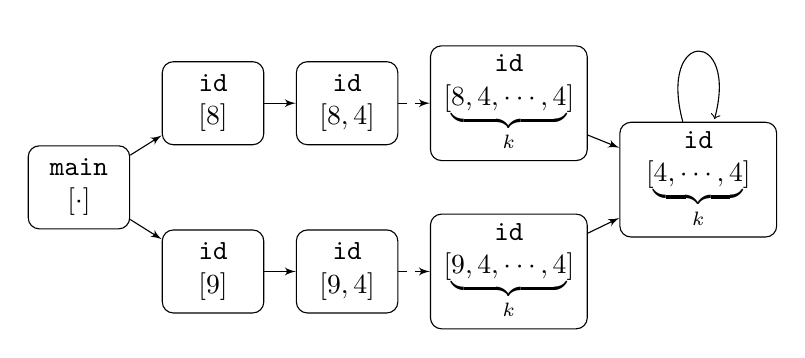
\begin{tikzpicture}
    \node [block] (main) {{\tt main} \\ $[\cdot]$};
    \node [block, above right=0cm and 0.4cm of main] (id1) {{\tt id}\\$[8]$};
    \node [block, below right=0cm and 0.4cm of main] (id2) {{\tt id}\\$[9]$};
    \node [block, right=0.4cm of id1] (id3) {{\tt id} \\$[8,4]$};
    \node [block, right=0.4cm of id2] (id4) {{\tt id} \\$[9,4]$};
    \node [block2, right=0.4cm of id3] (id5) {{\tt id}\\$[\underbrace{8,4,\cdots,4}_k]$};
    \node [block2, right=0.4cm of id4] (id6) {{\tt id}\\$[\underbrace{9,4,\cdots,4}_k]$};
    \node [block2, below right=-0.5cm and 0.4cm of id5] (id7) {{\tt id} \\$[\underbrace{4,\cdots,4}_{k}]$};

    \path [line] (main) -- (id1);
    \path [line] (main) -- (id2);
    \path [line] (id1) -- (id3);
    \path [line] (id2) -- (id4);
    \path [line, dashed] (id3) -- (id5);
    \path [line, dashed] (id4) -- (id6);
    \path [line] (id5) -- (id7);
    \path [line] (id6) -- (id7);
    \path [line] (id7) edge[loop above] ();
\end{tikzpicture}
}
\end{center}


\caption{Call-graph by $k$-CFA}
\label{fig:overview:kCFA}
\vspace{2ex}

\begin{center}
\resizebox{0.45\columnwidth}{!}{
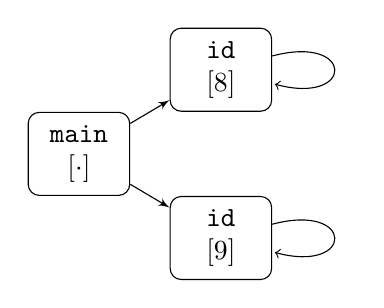
\begin{tikzpicture}
    \node [block] (main) {{\tt main}\\$[\cdot]$};
    \node [block, above right=0cm and 0.5cm of main] (id1) {{\tt id}\\$[8]$};
    \node [block, below right=0cm and 0.5cm of main] (id2) {{\tt id}\\ $[9]$};

    \path [line] (main) -- (id1);
    \path [line] (main) -- (id2);

    \path [line] (id1) edge[loop right] ();
    \path [line] (id2) edge[loop right] ();
\end{tikzpicture}
}
\end{center}
\caption{Call-graph by 1-CFA with tunneling}
\label{fig:overview:tunneling}
\end{subfigure}\qquad
\caption{Example and call-graphs constructed by the conventional
  $k$-call-site-sensitivity ($k$-CFA) and our 1-call-site-sensitivity
  with context tunneling}
\label{fig:overview}
\end{figure}




\myparagraph{Conventional Call-Site-Sensitivity}

The traditional $k$-call-site-sensitive analysis fails to prove the queries no matter what $k$ value is used.
Because the value of \texttt{i} can be any integer, the following set $K_{\infty}$ of infinite number of call-strings can be generated for method \texttt{id} at runtime:
\[
K_{\infty} = \myset{[8], [9], [8,4], [9,4], [8,4,4], [9,4,4], [8,4,4,4], [9,4,4,4], \dots}
\]
where, for example, $[8,4]$ denotes the context that method \texttt{id} was called along the sequence of
call-sites 8 and 4.
 The $k$-call-site-sensitive analysis approximates the call-strings in $K_{\infty}$ by their suffixes of length up to $k$. For example, when $k=2$, the analysis uses the following set $K_2$ of abstract contexts:
\[
K_2 = \myset{[8], [9], [8,4], [9,4], [4,4]}
\]
where an infinite number of contexts, $\myset{[8,4,4], [9,4,4], [8,4,4,4], [9,4,4,4],\dots}$, in $K_{\infty}$ are approximated by their common suffix $[4,4]$. The analysis analyzes the method \texttt{id} separately for each context in $K_2$. % producing the call-graph in Fig.~\ref{fig:overview}(b).
Although this approximation ensures termination, the analysis is now unable to differentiate the two separate calls to \texttt{id} at lines 8 and 9, causing the argument {\tt v} of {\tt id} to point to both objects {\tt A} and {\tt B} at the same time when the context becomes $[4,4]$. Thus, both objects get returned to both queries simultaneously, making the analysis fail to prove their cast safety.
Note that the analysis fails to prove the queries for any $k$ values, because all the context strings longer than $k$ are eventually
merged into a single context $[\underbrace{4,\dots,4}_{k}]$ (see
Fig.~\ref{fig:overview:kCFA}).


% the $k$-limited method is
% widely used in modern pointer
% analysis frameworks such as Doop~\cite{Bravenboer2009}.\minseok{redundant??}


% \minseok{
% 	Be aware that other kinds of context sensitivity like value context
% 	can prove the queries but	our goal is to overcome limitation of k-limiting context-sensitivity
% 	which is widely used.}
	
\myparagraph{Context Tunneling}

With context tunneling, however, even $1$-call-site sensitive analysis
becomes to prove the queries.
% Our idea to improve the analysis is to identify and maintain important
% context elements only.
The main weakness of the conventional
$k$-context-sensitive analysis is that it blindly updates the context
of a method at every call-site, thereby allowing important context
elements for the method to be easily overwritten by less important
ones.  In the example, distinguishing the two call-sites
at lines 8 and 9 is essential to proving the queries. However, this
information is eventually lost by repeatedly appending the less
important call-site 4 to the context of {\tt id}
(Fig.~\ref{fig:overview:kCFA}).
Our technique aims to overcome this weakness by maintaining important
context elements only during analysis. For example, we exclude the
call-site 4 from the context strings generated for method {\tt id} and
thus approximate the set $K_{\infty}$ to the set $K_T$ of contexts:
\[
K_T = \myset{[8], [9]}.
\]
Here abstract contexts $[8]$ and $[9]$ in $K_{T}$ denote the sets of concrete contexts
$\myset{[8], [8,4], [8,4,4], \dots}$ and
$\myset{[9], [9,4], [9,4,4], \dots}$ in $K_{\infty}$, respectively. The resulting
context-sensitive analysis with $K_{T}$ is able to prove the queries as it differentiates the two calls
to {\tt id} at lines 8 and 9 completely, producing the call-graph in
Fig.~\ref{fig:overview:tunneling}.

% With context tunneling, however, even $1$-call-site sensitive analysis
% is able to prove the queries.

\myparagraph{Challenge}

The example shows that the idea of context tunneling is potentially
powerful; even $1$-context-sensitivity with
tunneling can be as precise as
$\infty$-context-sensitivity. The goal of this chapter is to maximize
this tremendous, yet untapped, potential of the existing $k$-context-sensitive analysis.
However, achieving effective context tunneling in practice is
challenging. The effectiveness of the technique is very sensitive
to the choice of important context elements.  For example,
choosing the call-site 4, rather than call-sites 8 and 9, does not
work for the example program.  In the worst case, the analysis
precision degenerates into the context-insensitive case (e.g. when
selecting no context elements at all), becoming even inferior to the
ordinary
$k$-context-sensitive analysis.  Coming up with a good
heuristic rule for choosing important context elements is nontrivial;
hand-crafting such a rule not only requires a huge amount of
engineering effort and domain knowledge but also likely fails to
maximize the potential of the technique.
% adaptable as a fixed heuristic rule tuned for a particular situation
% may not be effective for other programs, analyses, or queries.


\myparagraph{Data-Driven Context Tunneling}


We address this challenge with a data-driven approach that
automatically learns a good heuristic rule for context tunneling from
a training set of programs.
Our aim is to generate a heuristic $\heuristic$,
% To do so, we first define a parameterized heuristic $\heuristic_\Pi$
% (where $\Pi$ is a parameter). $\heuristic_\Pi$
which takes a program and returns a relation $\TunnelingRelation$ on methods.
The relation contains a method pair $(m_1, m_2)$ if the calling context of
$m_1$ is more important than that of $m_2$. Thus, if $(m_1, m_2) \in
\TunnelingRelation$, the analysis applies context tunneling when $m_2$ is
invoked; that is, $m_2$ inherits the context of $m_1$ ignoring the current
context element. For the $k$-call-site-sensitivity example, $\heuristic_\Pi$
produces the relation $\TunnelingRelation = \myset{({\tt id}, {\tt id})}$,
which means that tunneling is applied when {\tt id} is called from {\tt id}.
As a result, the call-site 4, on which {\tt id} is called from {\tt id}, will
not be used as important context elements during analysis.  When {\tt main}
calls {\tt id}, however, the analysis updates the contexts as the ordinary
analysis since $({\tt main}, {\tt id}) \not\in \TunnelingRelation$.  In our
approach, the heuristic is parameterized and the parameter determines the
contents of the relation $\TunnelingRelation$.  The goal of our data-driven
technique is to characterize the two classes of methods: 1) methods that
increase the analysis precision by passing their contexts to others, and 2)
methods that increase the analysis precision by inheriting contexts from
others. Section~\ref{sec:learning} defines the learning problem and presents
an efficient algorithm to solve the problem.


%\subsection{Object-Sensitivity}
%
%The use of context tunneling is not limited to call-site-sensitivity.
%% Context tunneling is also effective for other flavors of
%% context-sensitivity.
%Below, we describe a typical situation where object-sensitivity
%benefits from context
%tunneling.
%
%%\lstset{
  language=Java,
  aboveskip=3mm,
  belowskip=3mm,
  showstringspaces=false,
  columns=flexible,
  basicstyle={\scriptsize\ttfamily},
  numbers=left,
  numbersep=5pt,
  numberstyle=\small\color{gray},
  keywordstyle=\color{blue},
  commentstyle=\color{dkgreen},
  stringstyle=\color{mauve},
  breaklines=true,
  breakatwhitespace=true,
  tabsize=3
}
\begin{figure}
\begin{subfigure}[b]{.9\columnwidth}
\begin{multicols}{2}
\centering
\begin{lstlisting}
class A {} class B {}
class C {
  public static void main (){
    ArrayList al1 = new ArrayList();//AL1
    ArrayList al2 = new ArrayList();//AL2

    al1.add(new A());
    al2.add(new B());

    Itr it1 = al1.iterator();
    Itr it2 = al2.iterator();

    A a = (A)it1.next();  //Query 1
    B b = (B)it2.next();  //Query 2
  }
}

class ArrayList{
  Object[] elementData = new Object[10];
  int size = 0;
  void add(Object e){
    elementData[size++] = e;
  }
  Itr iterator(){
    return new Itr(); //IT
  }
  class Itr{
    int cursor = 0;
    Object next(){
      return elementData[cursor++];
    }
  }
}
\end{lstlisting}
\end{multicols}
\caption{Example code}
\label{fig:obj:code}
\end{subfigure}
\begin{multicols}{2}
\begin{subfigure}[b]{.9\columnwidth}
\begin{center}
\resizebox{\columnwidth}{!}{
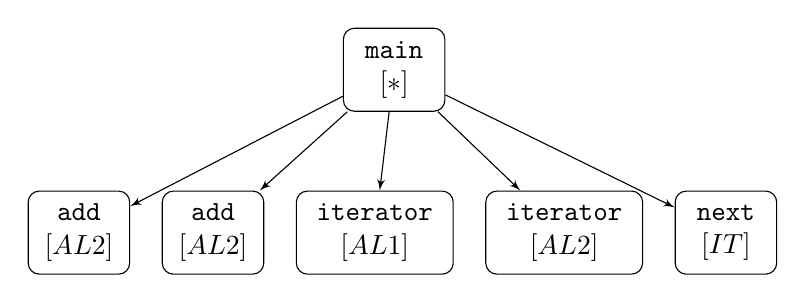
\begin{tikzpicture}
    \node [block] (main) {{\tt main}\\$[*]$};
    \node [block, below left=1cm and 2.7cm of main] (add1) {{\tt add}\\$[AL2]$};
    \node [block, right=0.4cm of add1] (add2) {{\tt add}\\$[AL2]$};
    \node [block2, right=0.4cm of add2] (iterator1) {{\tt iterator}\\ $[AL1]$};
    \node [block2, right=0.4cm of iterator1] (iterator2) {{\tt iterator}\\$[AL2]$};
    \node [block, right=0.4cm of iterator2] (next) {{\tt next}\\$[IT]$};

    \path [line] (main) -- (add1);
    \path [line] (main) -- (add2);
    \path [line] (main) -- (iterator1);
    \path [line] (main) -- (iterator2);
    \path [line] (main) -- (next);

\end{tikzpicture}
}
\end{center}
\caption{Call-graph by $1$-object-sensitive analysis}
\label{fig:obj:callgraph}
\end{subfigure}
\vfill\null
\columnbreak
\begin{subfigure}[b]{.9\columnwidth}
\begin{center}
\resizebox{\columnwidth}{!}{
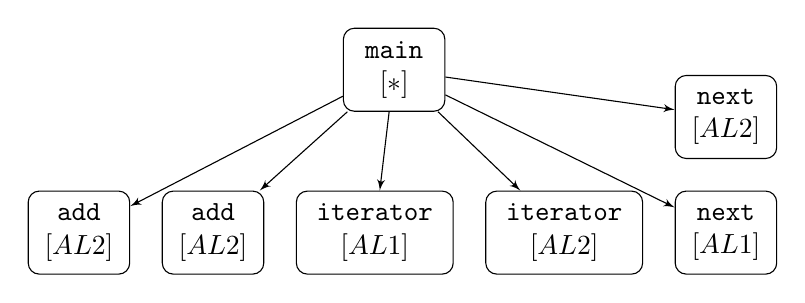
\begin{tikzpicture}
    \node [block] (main) {\tt main\\$[*]$};
    \node [block, below left=1cm and 2.7cm of main] (add1) {{\tt add}\\$[AL2]$};
    \node [block, right=0.4cm of add1] (add2) {\tt add\\$[AL2]$};
    \node [block2, right=0.4cm of add2] (iterator1) {\tt iterator\\$[AL1]$};
    \node [block2, right=0.4cm of iterator1] (iterator2) {\tt iterator\\$[AL2]$};
    \node [block, right=0.4cm of iterator2] (next1) {\tt next\\$[AL1]$};
    \node [block, above=0.4cm of next1] (next2) {\tt next\\$[AL2]$};

    \path [line] (main) -- (add1);
    \path [line] (main) -- (add2);
    \path [line] (main) -- (iterator1);
    \path [line] (main) -- (iterator2);
    \path [line] (main) -- (next1);
    \path [line] (main) -- (next2);

\end{tikzpicture}
}

\end{center}
\caption{Call-graph by $1$-object-sensitive analysis with tunneling}
\label{fig:obj:tunneling}
\end{subfigure}
\end{multicols}
\setlength{\abovecaptionskip}{-5pt}
\caption{Example code and callgraphs}
\label{fig:overviewObj}
\end{figure}

\myparagraph{Example Code for Object Sensitivity}
Example code in Fig.~\ref{fig:obj:code} present common pattern that 1-object-sensitive+heap
analysis lose precision. The main method use two data structure Arraylist, and it add
different data to each Arraylist. Main method makes iterator for each Arraylist and 
get data with iterators. The queries ask if two type casts at line 13 and 14 are
safe. 1-object-sensitive+heap analysis fails to prove the queries because
\texttt{next} method invoked in 13 and 14 are merged as
the method invocations have same context \texttt{IT}, 
constructing call-graph in Fig.~\ref{fig:obj:callgraph}. 

\myparagraph{Context Tunneling for Object sensitivity} 
With context tunneling, 1-object-sensitive+heap analysis can prove the queries. Note that Object sensitivity
has different flavor from call-site sensitivity; it updates context from heap context. Base
variable \texttt{it1} and \texttt{it2} point to same heap allocation but have different heap context: 
\texttt{AL1} and \texttt{AL2}. Applying context tunneling for \texttt{next} method make method call
at line 13 have context \texttt{AL1} and 14 have context \texttt{AL2},
resulting context sensitive analysis prove the queries with call-graph 
Fig.~\ref{fig:obj:tunneling}. 


%%% Local Variables:
%%% mode: latex
%%% TeX-master: "paper"
%%% End:

%\lstset{
%  language=Java,
%  aboveskip=3mm,
%  belowskip=3mm,
%  showstringspaces=false,
%  columns=flexible,
%  basicstyle={\scriptsize\ttfamily},
%  numbers=left,
%  numbersep=5pt,
%  numberstyle=\small\color{gray},
%  keywordstyle=\color{blue},
%  commentstyle=\color{dkgreen},
%  stringstyle=\color{mauve},
%  breaklines=true,
%  breakatwhitespace=true,
%  tabsize=3
%}
%\begin{figure}
%\begin{subfigure}[b]{0.9\columnwidth}
%\begin{multicols}{2}
%\centering
%\begin{lstlisting}
%class A {} class B {}
%class C {
%  public static void main (){
%    ArrayList al1 = new ArrayList();//AL1
%    ArrayList al2 = new ArrayList();//AL2
%
%    al1.add(new A());
%    al2.add(new B());
%
%    ArrayList.ListItr it1 = al1.iterator();
%    ArrayList.ListItr it2 = al2.iterator();
%
%    A a = (A)it1.next();  //Query 1
%    B b = (B)it2.next();  //Query 2
%  }
%}
%
%class ArrayList{
%  Object[] elementData = new Object[10];
%  int size = 0;
%  void add(Object e){
%    elementData[size++] = e;
%  }
%  ListItr iterator(){
%    return new ListItr(); //IT
%  }
%  class ListItr{
%    int cursor = 0;
%    Object next(){
%      return elementData[cursor++];
%    }
%  }
%}
%\end{lstlisting}
%\end{multicols}
%\caption{Example code}
%\label{fig:obj:code}
%\end{subfigure}
%\begin{multicols}{2}
%\begin{subfigure}[b]{.9\columnwidth}
%\begin{center}
%\resizebox{\columnwidth}{!}{
%\begin{tikzpicture}
%    \node [block] (main) {{\tt main}\\$[\cdot]$};
%    \node [block, below left=1cm and 2.7cm of main] (add1) {{\tt add}\\$[AL1]$};
%    \node [block, right=0.4cm of add1] (add2) {{\tt add}\\$[AL2]$};
%    \node [block2, right=0.4cm of add2] (iterator1) {{\tt iterator}\\ $[AL1]$};
%    \node [block2, right=0.4cm of iterator1] (iterator2) {{\tt iterator}\\$[AL2]$};
%    \node [block, right=0.4cm of iterator2] (next) {{\tt next}\\$[IT]$};
%
%    \path [line] (main) -- (add1);
%    \path [line] (main) -- (add2);
%    \path [line] (main) -- (iterator1);
%    \path [line] (main) -- (iterator2);
%    \path [line] (main) -- (next);
%
%\end{tikzpicture}
%}
%\end{center}
%\caption{Call-graph by $1$-object-sensitive analysis}
%\label{fig:obj:callgraph}
%\end{subfigure}
%\vfill\null
%\columnbreak
%\begin{subfigure}[b]{.9\columnwidth}
%\begin{center}
%\resizebox{\columnwidth}{!}{
%\begin{tikzpicture}
%    \node [block] (main) {\tt main\\$[\cdot]$};
%    \node [block, below left=1cm and 2.7cm of main] (add1) {{\tt add}\\$[AL1]$};
%    \node [block, right=0.4cm of add1] (add2) {\tt add\\$[AL2]$};
%    \node [block2, right=0.4cm of add2] (iterator1) {\tt iterator\\$[AL1]$};
%    \node [block2, right=0.4cm of iterator1] (iterator2) {\tt iterator\\$[AL2]$};
%    \node [block, right=0.4cm of iterator2] (next1) {\tt next\\$[AL1]$};
%    \node [block, above=0.4cm of next1] (next2) {\tt next\\$[AL2]$};
%
%    \path [line] (main) -- (add1);
%    \path [line] (main) -- (add2);
%    \path [line] (main) -- (iterator1);
%    \path [line] (main) -- (iterator2);
%    \path [line] (main) -- (next1);
%    \path [line] (main) -- (next2);
%
%\end{tikzpicture}
%}
%
%\end{center}
%\caption{Call-graph by $1$-object-sensitive analysis with tunneling}
%\label{fig:obj:tunneling}
%\end{subfigure}
%\end{multicols}
%\setlength{\abovecaptionskip}{-5pt}
%\caption{Example and call-graphs constructed by the conventional 1-object-sensitivity and our
%1-object-sensitivity with context tunneling}
%\label{fig:overviewObj}
%\end{figure}
%
%\myparagraph{Example Code}
%
%Fig.~\ref{fig:obj:code} shows
%a common code pattern that $1$-object-sensitivity with a context-sensitive heap
%loses precision, which is found frequently in data
%structure implementations such as List and Map.
%In the example code, we have four
%top-level classes, \texttt{A}, \texttt{B}, \texttt{C}, and
%\texttt{ArrayList}, and an inner class \texttt{ListIter} inside of the
%\texttt{ArrayList} class. The \texttt{ArrayList} class % , as the name suggests,
%% models on \texttt{java.util.ArrayList}, which is
%implements a resizable array.
%For simplicity, it maintains data in the % (fixed-size)
%\texttt{elementData} array and has the \texttt{add} method to append new data at
%the end of \texttt{elementData}. It also has the \texttt{iterator} method that
%returns an object of type \texttt{ListIter}, providing access to \texttt{elementData}.
%The \texttt{main} method in class \texttt{C} performs usual
%allocate-add-retrieve
%tasks using \texttt{ListIter}. The goal of the pointer
%analysis is to prove the safety of two type casts at lines 13
%and 14.
%
%\myparagraph{Conventional Object-Sensitivity}
%
%Conventional object-sensitivity analyzes different method calls
%separately for their base objects (and their heap contexts, if needed)~\cite{Smaragdakis2011}.  For
%example, when we analyze the \texttt{next} method at line 13,
%2-object-sensitivity creates the context $[\texttt{AL1},
%\texttt{IT}]$, where \texttt{IT} is the allocation-site of the base
%object (\texttt{it1}) and \texttt{AL1} is its heap context.
%Likewise, the
%method invocation at line 14 creates the context $[\texttt{AL2}, \texttt{IT}]$, enabling
%the analysis to distinguish the first and second calls to the same method. Using base objects
%as contexts makes object-sensitivity more favorable than
%call-site-sensitivity for object-oriented languages. However, it still
%updates contexts unconditionally at every method call and may lose important
%context elements when $k$ is not sufficiently large. For example, when we
%analyze the code with 1-object-sensitivity, the two calls to
%\texttt{next} are analyzed under the same context $[\texttt{IT}]$
%(Fig.~\ref{fig:obj:callgraph}).
%As a result, both objects \texttt{A} and \texttt{B} get returned to both
%queries simultaneously, making the analysis fail to prove the safety of type
%casting.
%
%
%
%\myparagraph{Object-Sensitivity with Context Tunneling}
%With context tunneling, however, even 1-object-sensitivity can prove the queries. Note that
%object-sensitivity has a different flavor from call-site-sensitivity; it
%updates the context with the heap context of the base object~\cite{Milanova2005, Milanova2002}. Base
%variables \texttt{it1} and \texttt{it2} point to the same heap allocation with different heap contexts: \texttt{AL1} and \texttt{AL2}. Applying context
%tunneling for the two method calls to \texttt{next} corresponds to
%propagating the heap contexts \texttt{AL1} and \texttt{AL2} at lines
%13 and 14, respectively, without modification.
%% makes the method call at line 13 to have
%% the context \texttt{AL1} and the method call at 14 to have the context \texttt{AL2}.
%The resulting context-sensitive analysis proves the queries with a call-graph
%shown in Fig.~\ref{fig:obj:tunneling}.


%%% Local Variables:
%%% mode: latex
%%% TeX-master: "paper"
%%% End:

%\section{Overview}
In this section, we illustrate how our approach learns a context sensitivity heuristic from codebases; the learned heuristic generate analysis strategy for unknown programs. 

\subsection{Our learning framework}
\myparagraph{Learning analysis heuristic from codebases}
Below graph depicts how our learning framework:
\begin{center}
\resizebox{0.7\columnwidth}{!}{
	\centering
	\begin{tikzpicture}
	\node [onlyText] (codebases) {\text{codebases $\vec{P}$}};
	\node [onlyText, right =
	 4.4cm of codebases]
	(minimalabs) {\text{minimal abstractions}};
	\node [onlyText, below = 1.4cm of minimalabs,align=center] (graphs) {\text{set of graphs}};
	\node [onlyText, below right = 0.2 and -1.0cm of minimalabs] (mytext) {\text{transforms to} \\ \text{set of graphs}};		
	\node [onlyText, left = 4.4cm of graphs] (heuristic) {\text{heuristic $\heuristic$}};	

	\path [line] (codebases) edge node[above] {$\text{learn minimal abstractions}$} (minimalabs);
	\path [line] (minimalabs) edge node[right] {} (graphs);	
	\path [line] (graphs) edge node[below] {$\text{learn heuristic graphs}$} (heuristic);
	\end{tikzpicture}
}
\end{center}
Suppose program in Fig~\ref{fig:codebase} is a given codebase. The program has an identity method {\tt h}.
Method {\tt f} calls {\tt h} twice with its parameter {\tt a} and a value from users. A method {\tt g} calls method {\tt f} with parameter 8. Method {\tt m} invokes {\tt f} with 8 and {\tt g} twice.
A query in method {\tt f} asks if the value of x is larger than 0. In real execution, it always holds because the value of x is 4 or 8. 
%To prove the query, we need 2-call-site-sensitivity. 
Our framework first learns minimal abstractions of the codebases. 
An abstraction maps each method in the codebase to an abstraction degree (e.g., 0, 1, or 2).
Minimal abstraction maps each method to an as small as possible one while the proves the query. 
In our example, the minimal abstraction is Fig~\ref{fig:minimal}; if we give lower abstraction degree to any of the method, the analysis fails to prove the query.



After it obtains minimal abstractions, our framework transforms each program component to a graph which can be obtained by a cheap analysis.
In our example, we use context-insensitive analysis to get call-graph (e.g., Fig~\ref{fig:callgraph}) and transforms each method in minimal abstraction to corresponding graph like Fig~\ref{fig:setOfGraph}.


From the sets of graphs in minimal abstractions, we transforms each graph to a small abstract graph.
The learned sets of abstract graphs are returned as a call-site-sensitivity heuristic heuristic;
it produces context sensitivity strategy for unknown programs.



%
%\begin{enumerate}
%	\item From the codebases, our framework obtain minimal abstraction for each program.
%	\item It transforms the minimal abstraction to a set of graphs.
%	\item It learns suitable abstract graphs from the extracted ones.
%	\item The learned abstract graphs becomes the heuristic; it generates an abstraction for unknown programs.
%\end{enumerate}

\begin{figure}
	\centering
	\begin{multicols}{2}
	\begin{lstlisting}
	class A{} class B{}
	class C{
	main(){
	  Container c1 = new Container();//C1
	  Container c2 = new Container();//C2
	
	  c1.add(new A());//A1
	  c1.add(new A());//A2
	  
	  c2.add(new B());//B1
	  c2.add(new B());//B2
	
	  Iterator it1 = c1.iterator();
	  Iterator it1 = c2.iterator();
	  A a = (A)it1.next();//query
	  B b = (B)it2.next();//query
	  }
	}
	class Container{
	  Object[] data = new Object[2];//O
	  int size = 0;
	  void add(Object e){
	    data[size++] = e;
	  }
	  Iterator iterator(){
	    return new Iterator();//It
	  } 
	}
	class Iterator{
	  Container container; cursor = 0;
	  Iterator(Container c){
	    container = c;}
	  Object next(){
	    return c.data[cursor++];}
	}
	\end{lstlisting}
	\end{multicols}
	\caption{Example to illustrate heap abstraction and context abstraction}
\end{figure}

\begin{figure}
	\begin{multicols}{2}
	\begin{subfigure}[t]{0.7\columnwidth}
		\begin{center}
			\resizebox{1.\columnwidth}{!}{
				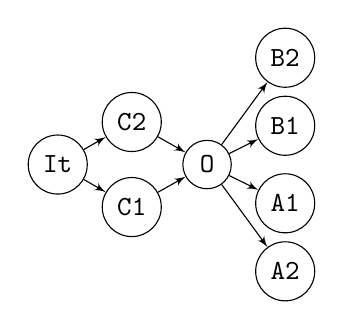
\begin{tikzpicture}
				\node [shape=circle,draw=black] (it) {{\tt It}};

				\node [shape=circle,draw=black, below right = 0.cm and 0.4cm of it] (c1) {{\tt C1}};				
				\node [shape=circle,draw=black, above right = 0.cm and 0.4cm of it] (c2) {{\tt C2}};

				\node [shape=circle,draw=black, right = 1.2cm of it] (o) {{\tt O}};				


				\node [shape=circle,draw=black, below right = 0.0cm and 0.5cm of o] (a1) {{\tt A1}};
				\node [shape=circle,draw=black, below = 0.1cm of a1] (a2) {{\tt A2}};

				\node [shape=circle,draw=black, above right = 0.0cm and 0.5cm of o] (b1) {{\tt B1}};
				\node [shape=circle,draw=black, above = 0.1cm of b1] (b2) {{\tt B2}};




				\path [line] (it) -- (c1);
				\path [line] (it) -- (c2);

				\path [line] (c1) -- (o);
				\path [line] (c2) -- (o);
				
				\path [line] (o) -- (a1);
				\path [line] (o) -- (a2);
				\path [line] (o) -- (b1);
				\path [line] (o) -- (b2);
				\end{tikzpicture}
			}
		\end{center}
		\caption{Points-to graph}
	\end{subfigure}
	
	
	\begin{subfigure}[t]{0.7\columnwidth}
		
		\begin{center}
			\resizebox{1.\columnwidth}{!}{
				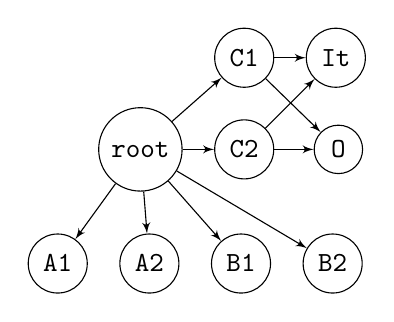
\begin{tikzpicture}
				\node [shape=circle,draw=black] (root) {{\tt root}};
						
				\node [shape=circle,draw=black, right =  0.4cm of root] (c2) {{\tt C2}};
				\node [shape=circle,draw=black, above= 0.4cm of c2] (c1) {{\tt C1}};		
				
				\node [shape=circle,draw=black, right = 0.5cm of c2] (o) {{\tt O}};				
				\node [shape=circle,draw=black, right = 0.4cm of c1] (it) {{\tt It}};				


				\node [shape=circle,draw=black, below left = 0.8cm and 0.4cm of root] (a1) {{\tt A1}};		
				\node [shape=circle,draw=black, right = 0.4cm of a1] (a2) {{\tt A2}};
				\node [shape=circle,draw=black, right = 0.4cm of a2] (b1) {{\tt B1}};
				\node [shape=circle,draw=black, right = 0.4cm of b1] (b2) {{\tt B2}};



				\path [line] (root) -- (c1);
				\path [line] (root) -- (c2);

				\path [line] (root) -- (a1);
				\path [line] (root) -- (a2);
				\path [line] (root) -- (b1);
				\path [line] (root) -- (b2);

				\path [line] (c1) -- (it);
				\path [line] (c1) -- (o);
				\path [line] (c2) -- (it);
				\path [line] (c2) -- (o);

				\end{tikzpicture}
			}
		\end{center}
		\caption{Object allocation graph}
	\end{subfigure}	
	\end{multicols}
	\caption{Points-to graph and object allocation graph produced by a cheap analysis (e.g., context-insensitive)}
\end{figure}






\begin{figure}[t]	
	\begin{multicols}{3}
		\begin{subfigure}[t]{1.0\columnwidth}
			\begin{center}
				\begin{lstlisting}[escapeinside={(*}{*)}]
int h(n) {ret n;}
void f(a){
  x = h(a);
  assert(x==4||x==8);//query
  y=h(input());
}
void g(){f(8);}
void m(){
  f(4);
  g();
  g();
}
\end{lstlisting}
\caption{Codebase}
\label{fig:codebase}
\end{center}
\end{subfigure}~\linebreak
		
		%\scalefont{0.9}
		\begin{subfigure}[b]{1.0\columnwidth}
			\begin{center}
				\resizebox{0.4\columnwidth}{!}{
					\begin{tikzpicture}
					\node [onlyText] (main) {\Large \text{Apply 2-call: \{h\}}\\\text{Apply 1-call: \{f\}}\\\text{Apply 0-call: \{g,m\}}};
					\end{tikzpicture}
				}
			\end{center}
			\caption{Minimal abstraction}
			\label{fig:minimal}
		\end{subfigure}
		\vspace{8pt}~\\

					
		\qquad\linebreak%\linebreak
		\begin{subfigure}[b]{1.0\columnwidth}
			\begin{center}
				\resizebox{0.5\columnwidth}{!}{
					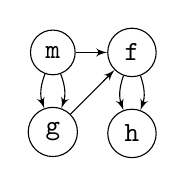
\begin{tikzpicture}
					\node [shape=circle,draw=black] (m) {{\tt m}};
					\node [shape=circle,draw=black, right = 0.4cm of m] (f) {{\tt f}};
					\node [shape=circle,draw=black, below = 0.4cm of m] (g) {{\tt g}};
					\node [shape=circle,draw=black, below = 0.4cm of f] (h) {{\tt h}};
					
					\path [line] (m) -- (f);
					\path [line] (f) edge [bend left=20] (h);
					\path [line] (f) edge [bend right=20] (h);
					\path [line] (g) -- (f);
					\path [line] (m) edge [bend left=20] (g);
					\path [line] (m) edge [bend right=20] (g);
					
					\end{tikzpicture}
				}
			\end{center}
			\caption{Call-graph of ci}
			\label{fig:callgraph}
		\end{subfigure}
	
	
	\columnbreak%\linebreak
		\begin{subfigure}[b]{1.0\columnwidth}
			\begin{center}
				\resizebox{0.5\columnwidth}{!}{
					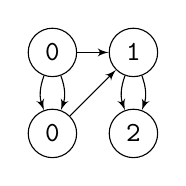
\begin{tikzpicture}
					\node [shape=circle,draw=black] (m) {{\tt 0}};
					\node [shape=circle,draw=black, right = 0.4cm of m] (f) {{\tt 1}};
					\node [shape=circle,draw=black, below = 0.4cm of m] (g) {{\tt 0}};
					\node [shape=circle,draw=black, below = 0.4cm of f] (h) {{\tt 2}};
					
					\path [line] (m) -- (f);
					\path [line] (f) edge [bend left=20] (h);
					\path [line] (f) edge [bend right=20] (h);
					\path [line] (g) -- (f);
					\path [line] (m) edge [bend left=20] (g);
					\path [line] (m) edge [bend right=20] (g);
					
					\end{tikzpicture}
				}
			\end{center}
			\caption{Graph with a minimal abstraction}
			\label{fig:graphmin}
		\end{subfigure}
%			
%	\begin{subfigure}[b]{1.0\columnwidth}
%		\begin{center}
%			\resizebox{0.7\columnwidth}{!}{
%				\begin{tikzpicture}
%
%				\node [shape=circle,draw=black] (m) {};
%				\node [onlyText, below left = -0.02cm and
%				1.5cm of f] (depth2) {\Large \text{Apply 2-call:\{$\qquad\quad$\}}};
%				\node [shape=circle,draw=black, right = 0.4cm of m] (f) {};
%				\node [shape=circle,draw=black, below = 0.4cm of m] (g) {};
%				\node [shape=circle,draw=black, below = 0.4cm of f,fill=gray] (h) {};
%				
%
%
%
%
%				\path [line] (m) -- (f);
%				\path [line] (f) edge [bend left=20] (h);
%				\path [line] (f) edge [bend right=20] (h);
%				\path [line] (g) -- (f);
%				\path [line] (m) edge [bend left=20] (g);
%				\path [line] (m) edge [bend right=20] (g);
%				
%				
%				\node [shape=circle,draw=black,below = 1.cm of m] (m2) {};
%				\node [shape=circle,draw=black, right = 0.4cm of m2,fill=gray] (f2) {};
%				\node [onlyText, below left = 0.05cm and
%				1.3cm of f2] (depth1) {\Large \text{Apply 1-call:\{$\qquad\quad$\}}};
%				\node [shape=circle,draw=black, below = 0.4cm of m2] (g2) {};
%				\node [shape=circle,draw=black, below = 0.4cm of f2] (h2) {};
%				
%				\path [line] (m2) -- (f2);
%				\path [line] (f2) edge [bend left=20] (h2);
%				\path [line] (f2) edge [bend right=20] (h2);
%				\path [line] (g2) -- (f2);
%				\path [line] (m2) edge [bend left=20] (g2);
%				\path [line] (m2) edge [bend right=20] (g2);
%				
%							
%				\end{tikzpicture}
%			}
%		\end{center}
%		\caption{Graphs}
%		\label{fig:setOfGraph}
%	\end{subfigure}~\\
	\vspace{8pt}~\\
	\vspace{8pt}~\\
	

	\begin{subfigure}[b]{1.0\columnwidth}
		\begin{center}
			\resizebox{1\columnwidth}{!}{
				\begin{tikzpicture}

				\node [] (f) {};
				\node [shape=ellipse,draw=black, right = 0.4 of f,fill=gray] (h) {((2,2),(0,0))};
				\node [onlyText, left = -0.1cm of f] (depth2) {\Large \text{Apply 2-call:\{$\qquad\qquad\qquad\quad$\}}};

				\node [shape=ellipse,draw=black, below = .5cm of f,fill=gray] (f2) {((2,2),(2,2))};
				\node [shape=ellipse,draw=black, right = 0.4 of f2] (h2) {((2,2),(0,0))};
				\node [onlyText, left = 0.5cm of f2] (depth1) {\Large \text{Apply 1-call:\{$\qquad\qquad\qquad\qquad\qquad\qquad\quad$\}}};
				\path [line] (f2) edge [] (h2);
%				\node [shape=ellipse, above left = 0.1 and 0.3 of f2] (blank1) {};
%				\node [shape=ellipse, below left = 0.1 and 0.3 of f2] (blank2){};				



%				\path [line] (f) edge [bend left=20] (h);
%				\path [line] (f) edge [bend right=20] (h);


%				\path [line] (f2) edge [bend left=20] (h2);
%				\path [line] (f2) edge [bend right=20] (h2);

%				\path [line] (blank1) edge  (f2);
%				\path [line] (blank2) edge  (f2);
				
				
				
				\end{tikzpicture}
			}
		\end{center}
		\caption{Heuristic graphs}
	\end{subfigure}
	
	\end{multicols}
	\vspace{-1em}
	\caption{How our learning framework obtains a heuristic}
\end{figure}




\myparagraph{How learned heuristic works}
We illustrate how learned heuristic generate analysis strategy with Fig~\ref{fig:heuristicWork}.
Suppose Fig~\ref{fig:unknown} is given unknown program and Fig~\ref{fig:learnedHeuristic} is learned heuristic from codebases.
To obtain analysis strategy, we run context insensitive analysis and obtain call-graph in Fig~\ref{fig:unknwon:callgraph}.
The learned heuristic assign 2-call-site-sensitivity to the method {\tt h} as
the node {\tt h} in Fig~\ref{fig:unknwon:callgraph} has no out going edges and has 2 incoming edges from a node like Apply 2-call in Fig~\ref{fig:learnedHeuristic}.
The heuristic assign 1-call-site-sensitivity to the method {\tt f} as
the node {\tt f} in in Fig~\ref{fig:unknwon:callgraph} has two out going edges to a node and has two incoming edges like Apply 1-call in Fig~\ref{fig:learnedHeuristic}.
Other methods belong to 0-call as node {\tt m} and {\tt d} has different form from abstract graphs in Fig~\ref{fig:learnedHeuristic}.
It generates call-site-sensitivity strategy in Fig~\ref{fig:strategy}. It produces context abstraction in Fig~\ref{fig:unknown:callGraph} and it can prove the queries.




\begin{figure}[t]	
	\begin{multicols}{3}
		\begin{subfigure}[t]{1.0\columnwidth}
			\begin{center}
				\begin{lstlisting}[escapeinside={(*}{*)}]
d(){}
h(v){
  return 2*v;}
f(v){
  r = h(v);
  return h(r);}
main(){
  q1 = f(1);
  q2 = f(2);
  assert(q1 == 4);//query1
  assert(q2 == 8);//query2
  d();
  d();
  d();
}
				\end{lstlisting}
				\caption{Unknown program}
				\label{fig:unknown}
			\end{center}
		\end{subfigure}
			
			\columnbreak%\linebreak
		
		%\scalefont{0.9}
%		\begin{subfigure}[b]{1.0\columnwidth}
%			\begin{center}
%				\resizebox{0.4\columnwidth}{!}{
%					\begin{tikzpicture}
%					\node [onlyText] (main) {\Large \text{Apply 2-call: \{h\}}\\\text{Apply 1-call: \{f\}}\\\text{Apply 0-call: \{g,m\}}};
%					\end{tikzpicture}
%				}
%			\end{center}
%			\caption{Minimal abstraction}
%		\end{subfigure}
%		\vspace{8pt}~\\
%		\vspace{8pt}~\\
		\begin{subfigure}[b]{0.8\columnwidth}
			\begin{center}
				\resizebox{1.2\columnwidth}{!}{
					\begin{tikzpicture}
					
					\node [] (f) {};
					\node [shape=ellipse,draw=black, right = 0.4 of f,fill=gray] (h) {((2,2),(0,0))};
					\node [onlyText, left = -0.1cm of f] (depth2) {\Large \text{Apply 2-call:\{$\qquad\qquad\qquad\quad$\}}};
					
					\node [shape=ellipse,draw=black, below = .5cm of f,fill=gray] (f2) {((2,2),(2,2))};
					\node [shape=ellipse,draw=black, right = 0.4 of f2] (h2) {((2,2),(0,0))};
					\node [onlyText, left = 0.5cm of f2] (depth1) {\Large \text{Apply 1-call:\{$\qquad\qquad\qquad\qquad\qquad\qquad\quad$\}}};
					\path [line] (f2) edge [] (h2);
					\end{tikzpicture}
				}
			\end{center}
			\caption{Learned heuristic graphs}
			\label{fig:learnedHeuristic}
		\end{subfigure}		
		\vspace{8pt}~\\
		\vspace{8pt}~\\
				
			
		\qquad\linebreak%\linebreak
		\begin{subfigure}[b]{.7\columnwidth}
			\begin{center}
				\resizebox{.8\columnwidth}{!}{
					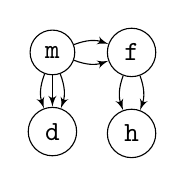
\begin{tikzpicture}
					\node [shape=circle,draw=black] (m) {{\tt m}};
					\node [shape=circle,draw=black, right = 0.4cm of m] (f) {{\tt f}};
					\node [shape=circle,draw=black, below = 0.4cm of m] (d) {{\tt d}};
					\node [shape=circle,draw=black, below = 0.4cm of f] (h) {{\tt h}};
					
					\path [line] (m) edge [bend left=20] (f);
					\path [line] (m) edge [bend right=20] (f);
					\path [line] (f) edge [bend left=20] (h);
					\path [line] (f) edge [bend right=20] (h);
					\path [line] (m) edge [bend left=20] (d);
					\path [line] (m) edge [bend right=20] (d);
					\path [line] (m) edge (d);
										
					\end{tikzpicture}
				}
			\end{center}
			\caption{Call-graph of ci}
			\label{fig:unknwon:callgraph}
		\end{subfigure}~\\




		\columnbreak%\linebreak

		\begin{subfigure}[b]{1\columnwidth}
			\begin{center}
				\resizebox{0.5\columnwidth}{!}{
					\begin{tikzpicture}
					\node [onlyText] (main) {\Large \text{Apply 2-call: \{h\}}\\\text{Apply 1-call: \{f\}}\\\text{Apply 0-call: \{d,m\}}};
					\end{tikzpicture}
				}
			\end{center}
			\caption{Generated abstraction}
			\label{fig:strategy}
		\end{subfigure}~\\
		\vspace{8pt}~\\
		

		\begin{subfigure}[b]{1\columnwidth}
			\begin{center}
				\resizebox{.8\columnwidth}{!}{
					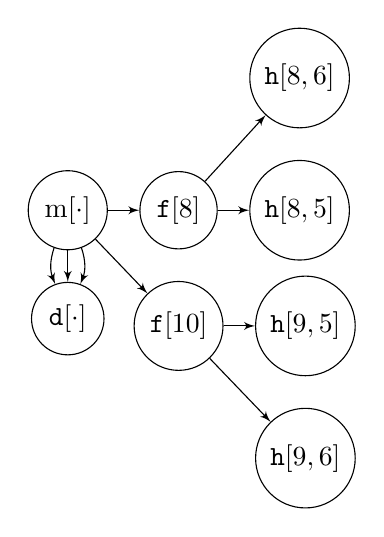
\begin{tikzpicture}
					\node [shape=circle,draw=black] (m) {m$[\cdot]$};
					\node [shape=circle,draw=black, right = 0.4cm of m] (f1) {{\tt f$[8]$}};
					\node [shape=circle,draw=black, below = 0.4cm of f1] (f2) {{\tt f$[10]$}};
					\node [shape=circle,draw=black, right = 0.4cm of f1] (h1) {{\tt h$[8,5]$}};
					\node [shape=circle,draw=black, above = 0.4cm of h1] (h11) {{\tt h$[8,6]$}};
					
					\node [shape=circle,draw=black, right = 0.4cm of f2] (h2) {{\tt h$[9,5]$}};
					\node [shape=circle,draw=black, below = 0.4cm of h2] (h22) {{\tt h$[9,6]$}};
					
					\node [shape=circle,draw=black, below = 0.4cm of m] (d) {{\tt d$[\cdot]$}};

					
					\path [line] (m) edge (f1);
					\path [line] (m) edge (f2);					
					\path [line] (f1) edge (h1);
					\path [line] (f2) edge (h2);
					\path [line] (f1) edge (h11);
					\path [line] (f2) edge (h22);
					\path [line] (m) edge [bend left=20] (d);
					\path [line] (m) edge [bend right=20] (d);
					\path [line] (m) edge (d);
					
					\end{tikzpicture}
				}
			\end{center}
			\caption{Call-graph}
			\label{fig:unknown:callGraph}
		\end{subfigure}~\\
		
		

		
	\end{multicols}
	\vspace{-1em}
	\caption{How learned heuristic generates analysis strategy}
	\label{fig:heuristicWork}
\end{figure}


%\section{Context sensitive Context Tunneling}
\begin{comment}
\begin{figure}
\begin{multicols}{2}
\begin{lstlisting}
0:   Class A{} Class B{}
1:   Object id1(Object v, int i){
2:     return v;
3:   }
4:   Object id2(Object v, int i){
5:     return id1(v);
6:   }
7:  void main(){
8:    A a1 = (A)id1(new A());//Q1
9:    B b1 = (B)id1(new B());//Q2
10:   A a1 = (A)id2(new A());//Q1
11:   B b1 = (B)id2(new B());//Q2
12:   return;}
\end{lstlisting}
(a) Example Code\\
\begin{center}


\includegraphics[width=6cm,height=6cm,keepaspectratio]{figures/ctxTunnel.pdf}\\
(c) Context-sensitive tunneling
\end{center}
\end{multicols}
\caption{Tunneling considering context}
\label{fig:ExampleCode}
\end{figure} 
\end{comment}
%\newpage

\section{Pointer Analysis with Context Tunneling} \label{sec:tunneling}
Now, we formally describe the idea of context tunneling on the top the analysis rule in Figure~\ref{pre:baseline-rules}.
%\subsection{Analysis with Context Tunneling}\label{sec:tunneling-analysis}
%Now we describe context tunneling on top of the generic context-sensitive analysis.
We assume that a binary relation $\TunnelingRelation$ on methods,
called tunneling relation, is given prior to the analysis:
% The idea of tunneling is simple: compare the
% parent and child contexts and use the more important one as the
% calling context of the called method.  We do so by using a binary
% relation
% $\TunnelingRelation$ on methods, called tunneling relation:
\[
  \TunnelingRelation \subseteq \Methods \times \Methods.
\]
Intuitively, $\TunnelingRelation$ relates the parent and child methods
that require context tunneling. Suppose that a method
$m_2$ is called during analysis where its parent method is $m_1$. If
$m_1$ and $m_2$ are related by $\TunnelingRelation$, i.e., $(m_1,m_2) \in \TunnelingRelation$, we apply context tunneling by
reusing the context of the parent method ($m_1$) in analyzing the
child method ($m_2$) without creating a new context for $m_2$.  Given
a tunneling relation $\TunnelingRelation$, the analysis rule for
performing context tunneling is defined in
Figure~\ref{fig:tunneling-rules}. All the existing rules except for
method calls are carried over to the new analysis without any modifications.
The rule for method call in Figure~\ref{pre:baseline-rules} is
replaced by the rule in Figure~\ref{fig:tunneling-rules}, where the
only difference is in the way of constructing the child context
$\ctx'$. If $(p,m) \not\in \TunnelingRelation$ (i.e. tunneling
disabled), we update the calling context as the conventional $k$-context-sensitive
analysis does. Otherwise, when $(p,m)\in \TunnelingRelation$
(i.e. tunneling enabled), we just pass the parent context $\pctx$ to
the child method (i.e. $\ctx' = \pctx$) without appending the current
context element to $\pctx$.
% Note that the ordinary $k$-context-sensitive analysis and
% context-insensitive analysis are special cases with
% $\TunnelingRelation = \emptyset$ and
% $\TunnelingRelation = \Methods \times \Methods$, respectively.


Although the idea of context tunneling is simple, realizing effective
tunneling in practice is challenging. We found that the performance of
context tunneling is very sensitive to the choice of the tunneling
relation; with a good relation, context tunneling is able to improve the
baseline analysis significantly but, with an inappropriate choice, the analysis
becomes even inferior to the context-insensitive analysis.  Manually finding a general heuristic rule to
generate an optimal tunneling relation for a given program was
difficult for real-world Java programs.
The goal of Section~\ref{tunneling:learning} is to address this challenge
with a data-driven technique that automatically learns a good
tunneling heuristic from data.

\begin{figure}[t]
  \[
    \begin{array}{c}
      \infer[]
      {
      \begin{array}{c}
        \ctx' \in \Reachable ({m}) \quad
        ({\heap}, {\hctx}) \in  \VarPointsTo ({m_{\this}}, {\ctx'}) \\
        \VarPointsTo({\it arg}, \ctx) \subseteq \VarPointsTo(m_{\it param}, \ctx')
        \quad
        \VarPointsTo(m_{\it return}, \ctx') \subseteq \VarPointsTo(x, \ctx)\\
        (\invo, \ctx, m, \ctx') \in \CallGraph
      \end{array}
      }{
      \begin{array}{c}
        {\it \invo : x = y.\sig({\it arg})} \quad
        \ctx \in    \Reachable ({\methof(\invo)}) \\
        ({\heap}, {\hctx})\in  \VarPointsTo ({\it y},\ctx) \quad
        t = {\typeof}(\heap)  \quad m = {\lookup}(t, \sig) \\
(e, {\pctx}, p) = \parent(\heap,\hctx, \invo, \ctx) \quad
        \ctx' = \left\{
        \begin{array}{l@{\quad}l}
          \truncateCtx{\appendCtx{{ \pctx}}{{e}}}{\CallDepth}
          & \mbox{if}~(p,m)\not\in \TunnelingRelation \\
          \truncateCtx{\pctx}{\CallDepth}     & \mbox{if}~(p,m)
                                                \in \TunnelingRelation
        \end{array}
                                                          \right.
      \end{array}
                                                          }
    \end{array}
  \]
  \caption{Context-sensitive pointer analysis with tunneling}
\label{fig:tunneling-rules}
\end{figure}

%%% Local Variables:
%%% mode: latex
%%% TeX-master: "paper"
%%% End:

\section{Learning Context-Tunneling Heuristics}\label{tunneling:learning}

Now, we present a machine-learning algorithm specialized for
generating good context tunneling heuristics from a dataset
of programs.


 % Although the
% idea of context tunneling is simple, realizing effective tunneling in
% practice is challenging. The performance of context tunneling depends
% on the choice of the tunneling relation $\TunnelingRelation$, but
% manually designing a heuristic rule to generate $\TunnelingRelation$
% for a given program is nontrivial and likely ends up with costly or
% imprecise results.  Our goal is to address this challenge by
% developing a machine-learning algorithm that learns
% context-tunneling heuristics from data.


\subsection{Parametric Program Analysis} \label{tunneling:setting}

Let us first encapsulate our analysis in Section~\ref{sec:tunneling}
as a parametric program analysis~\cite{Liang2011learning}.  Let
$P \in \Program$ be a program to analyze. Let $\Methods_P$ be the set
of methods in $P$.  Then, we can define the set $\tspace_P$ of all
tunneling relations for $P$ as follows:
\[
 \TunnelingRelation \in \tspace_P = \power{\Methods_P \times \Methods_P}.
\]
The set $\tspace_P$ forms the parameter space of the analysis for $P$,
where an element $\TunnelingRelation \in \tspace_P$ --- a set of
method pairs --- represents a tunneling relation.  Abstractions are
ordered by set inclusion.  For each pair $(m_1,m_2)$ of parent and
child methods in $\TunnelingRelation$, we apply context-tunneling by
reusing the calling context of the parent method ($m_1$) when analyzing the
child method ($m_2$) without creating a new context for $m_2$.  The abstraction
space covers the conventional context-insensitive and -sensitive
analyses: with $\TunnelingRelation = \emptyset$, the analysis becomes
an ordinary $k$-context-sensitive analysis, and with
$\TunnelingRelation = \Methods_P \times \Methods_P$, the analysis
equals to the context-insensitive analysis.

We assume that a set $\Assertion_P$ of assertions is given together
with the input program $P$.  For instance, $\Assertion_P$ may denote the set of all type casts in
$P$ and the analysis attempts to prove that they do not fail at
runtime (i.e. no down-casting failures).  Then,
we can model pointer analysis for $P$ by the function $F_P$:
\[
  F_P \in \tspace_P \to \power{\Assertion_P} \times \mbn.
\]
Given a program $P$ and a tunneling relation
$\TunnelingRelation \in \tspace_P$, $F_P(\TunnelingRelation)$ returns
the set $Q \subseteq \Assertion_P$ of proved assertions and the
analysis time $n \in \mbn$ represented by a natural number (e.g. time
took to analyze the program).  We define two projection functions:
$\proved(F_P(\TunnelingRelation))$ and
$\cost(F_P(\TunnelingRelation))$ denote the set of proved assertions
($Q$) and the analysis cost ($n$) of the analysis
$F_P(\TunnelingRelation)$, respectively.

% Once $\heuristic$ is generated, it can be used to analyze previously
% unseen program $P$ with $F_P (\heuristic(P))$.  We aim to learn a
% tunneling heuristic $\heuristic$ such that the analysis
% $F_P(\heuristic(P))$ improves the precision as much as possible while
% retaining the cost of the baseline analysis
% $F_P(\emptyset)$ (i.e. the ordinary $k$-context-sensitive analysis).

\myparagraph{Non-Monotonicity}

One noticeable property of context tunneling is non-monotonicity.  Note
that existing parametric program analyses are typically monotone with respect to
their parameters; that is, the analysis precision is monotonically
increasing (or decreasing) with respect to the parameters of the
analysis
(e.g.~\cite{Liang2011learning,JeJeChOh17,Zhang2014,Liang2011}).  That
is, if $p \sqsubseteq p'$ then
$\proved(F_P(p)) \subseteq \proved(F_P(p'))$ (or
$\proved(F_P(p)) \supseteq \proved(F_P(p'))$). For example, in a
selective context-sensitive analysis~\cite{JeJeChOh17}, making more
methods context-sensitive always increases precision.  In our case,
however, the analysis is not monotone with respect to the parameters
(i.e. context-tunneling relations). That is,
$\TunnelingRelation \subseteq \TunnelingRelation'$ does not imply
$F_P(\TunnelingRelation) \subseteq F_P(\TunnelingRelation')$ or
$F_P(\TunnelingRelation) \supseteq F_P(\TunnelingRelation')$.  Consequently, neither $F_P(\emptyset)$ nor
$F_P(\Methods_P\times\Methods_P)$ --- the conventional
$k$-context-sensitive analysis and context-insensitive analysis --- is
the most precise one in the parameter space of context tunneling.
As we describe in
Section~\ref{tunneling:learning-algorithm}, this unusual property makes
learning challenging; in particular, we cannot use the existing
learning algorithms (e.g.~\cite{JeJeChOh17,Liang2011learning}) that
exploit the monotonicity of analysis.


\subsection{Machine-Learning Model for Context Tunneling}


%\myparagraph{Parameterized Heuristic}

Our goal is to learn a {\em tunneling heuristic}, denoted
$\heuristic$, from a dataset of programs, which takes a program $P$
and returns a tunneling relation for $P$:
\[
  \heuristic(P) \in \power{\Methods_P \times \Methods_P}.
\]
To generate such a heuristic automatically, we need to define a space
of possible tunneling heuristics, called model or inductive bias in
the machine learning community.  A standard
method is to define the space by a generic heuristic with free
parameters, reducing the problem of generating a good heuristic to the
problem of finding appropriate parameter values.  There is a number of
different ways to define such a parameterized heuristic. For example,
we can use a linear combination of input features~\cite{Oh2015} or a
non-linear, disjunctive combination~\cite{JeJeChOh17}. We take the latter approach because the
non-linear method is known to be more effective for pointer analysis
than the simple linear approach~\cite{JeJeChOh17}.

Following \cite{JeJeChOh17},
we use a boolean formula over atomic features as a model parameter.
Let us assume that a set of {\em atomic features} is given:
$\afeatures = \myset{\afeat_1, \afeat_2, \dots, \afeat_n}$, where a feature $\afeat_i$ describes a property of
methods. It is a function from programs to predicates on
methods:
\[
\afeat_i(P) : \Methods_P \to \myset{\true,\false}.
\]
For example, a feature may express the set of methods that have
heap allocation in their bodies. We shortly present our atomic features in
detail.
Given a set of atomic features, we can express more complex features
of methods by combining the atomic features.
We combine them with
a boolean formula $f$ in disjunctive normal form, i.e., a disjunction of conjunctions
of literals:
\[
f = \bigvee_i \bigwedge_j l_{i,j}
\]
where $l_{i,j}$ is a literal: $\true$, $\false$, atomic feature $a \in \afeatures$,
or their negations.
Note that the meaning of a boolean formula is a set of methods.
Given a program $P$ and a formula $f =\bigvee_i \bigwedge_j l_{i,j}$, let $\sem{f}_P$ be the set of methods
on which the formula $f$ evaluates to true: $\sem{f}_P = \bigcup_i
\bigcap_j \sem{l_{i,j}}_P$ where $\sem{\true}_P = \Methods_P$,
$\sem{\false}_P = \emptyset$, $\sem{\afeat_i}_P = \myset{m \in
 \Methods_P \mid \afeat_i(P)(m) = \true}$, and $\sem{\neg a_i}_P =
 \Methods_P \setminus \sem{a_i}_P$.
In the rest of this chapter, we often represent a formula in
disjunctive normal form by a set of sets of literals. For example, the formula
$f = (a_1 \land a_2) \vee (\neg a_3 \land a_4)$ can be
represented by $\myset{\myset{a_1,a_2}, \myset{\neg a_3,a_4}}$.



Our model uses two boolean formulas $\params = \langle f_1,f_2
\rangle$ and generates the tunneling relation for a given program $P$ as follows:
\begin{equation}\label{eq:heuristic}
\heuristic_{\params} (P) = \myset{(m_1,m_2) \in \Methods_P \times
  \Methods_P \mid
  m_1 \in \sem{f_1}_P \vee m_2 \in \sem{f_2}_P}.
\end{equation}
The generated relation includes a pair $(m_1, m_2)$ of methods if
$m_1 \in \sem{f_1}_P$ or $m_2 \in \sem{f_2}_P$.
This conditions says that we apply context tunneling when
$m_1$ is implied by $f_1$ or $m_2$ by $f_2$. Intuitively, $f_1$ denotes the set of methods that improve the
analysis performance by passing their contexts to child methods, and
$f_2$ describes the methods that benefit by reusing the contexts of
their parent methods. The goal of our learning algorithm is to
discover the characteristics of such methods, represented by boolean
combinations ($f_1$ and $f_2$) of features, that maximize the performance of
the heuristic.

\begin{table}[t]
     \centering	\scriptsize
    \caption{Atomic features used in evaluation}
    \label{tbl:features}
\begin{tabular}{c}
    \begin{tabular}{clcclcclcclccl}
        \toprule
        \multicolumn{14}{c}{Class A (Signature features)} \\
        \midrule
        A1 & ``java'' &\quad& A2 & ``lang'' &\quad& A3 & ``sun'' &\quad& A4 & ``()'' &\quad& A5 & ``void'' \\
        A6 & ``security'' &\quad& A7 & ``int''  &\quad&  A8 & ``util'' &\quad& A9 & ``String'' &\quad&  A10 & ``init'' \\
        \bottomrule
    \end{tabular}
%\quad
%	\begin{tabular}{clclcl}
%		\toprule
%		\multicolumn{6}{c}{Class B (Statement features)} \\
%		\cmidrule(lr){1-6}
%		 B1 & Assign & B6 &
%		Breakpoint & B11 & Lookup \\
%		 B2 & Identity & B7 &
%		EnterMonitor & B12 & Nop \\
%		 B3 & Invoke & B8 &
%		ExitMonitor & B13 & Ret \\
%		 B4 & Return & B9 &
%		Goto & B14 & ReturnVoid \\
%		 B5 & Throw & B10 &
%		If & B15 & TableSwitch \\
%		\bottomrule
%	\end{tabular}
\\
\\
    \begin{tabular}{clcl}
        \toprule
        \multicolumn{4}{c}{Class B (Additional features)} \\
        \midrule
%          B1 & Methods contained in nested class  			& B8 & Methods containing virtual method invocation\\
% B2 & Methods taking multiple arguments 			& B9 & Static method \\
% B3 & Methods containing array load 				& B10 & Methods containing a single heap allocation \\
% B4 & Methods containing local assignments 			& B11 & Methods taking an argument of Object type \\
% B5 & Methods containing local variables 			& B12 & Methods containing multiple heap allocations \\
% B6 & Methods containing field store 				& B13 & Methods contained in a large class\\
% B7 & Methods containing static method invocation\\

 B1 & Methods contained in nested class  			& B7 & Methods containing static method invocation\\
 B2 & Methods taking multiple arguments 			& B8 & Methods containing virtual method invocation\\
 B3 & Methods containing array load 				& B9 & Static method \\
 B4 & Methods containing local assignments 			& B10 & Methods containing a single heap allocation \\
 B5 & Methods containing local variables 			& B11 & Methods taking an argument of Object type \\
 B6 & Methods containing field store 				& B12 & Methods containing multiple heap allocations \\
 & & B13 & Methods contained in a large class\\

      %    \#11 & Methods contained in inner class\\
      %    \#12 & Methods taking multiple arguments\\
      %   \#13 & Methods containing array load \\ % \textsc{LoadArrayIndex}
      %   % instruction\\
      %    \#14 & Methods containing local assignments \hakjoo{what is
      %           ``local assignment''?}\\
      %    \#15 & Methods containing local variables \\
      %    \#16 & Methods containing field store\\ % \textsc{StoreInstanceField} instruction\\
      %    \#17 & Methods containing static method invocation\\
      %    \#18 & Methods containing virtual method invocation\\
      %    \#19 & Methods containing a single heap allocation%  \hakjoo{single heap
      %           % alloc?} \\ &\minseok{yes only one heap allocation}
      % \\
      %    \#20 & Methods taking an argument of the ``Object'' type \\
      %    \#21 & Methods containing multiple heap allocations%  \hakjoo{diff with
      %           % \#19?}\\ &\minseok{Yes, 19 $\subset$ 21}
      % \\
      %    \#22 & Methods contained in a large class (\#Methods~$>$~20) \\
      %    \#23 & Static methods \\
        \bottomrule
    \end{tabular}
\end{tabular}
\end{table}


\myparagraph{Atomic Features}\label{sec:features}

Table~\ref{tbl:features} shows 23 atomic features we have used in learning.
Each feature in Table~\ref{tbl:features} describes a syntactic
property of Java method definitions.  The features are classified into
two types: signature features (Class A) and additional
features (Class B).  Signature features (A1 -- A10) came from the existing work~\cite{JeJeChOh17} and
additional features (B1 -- B13) have been newly designed in this work.
Signature features consist of strings that most frequently appear in
method signatures from the DaCapo suite~\cite{Blackburn2006}. For example, the feature A5
(``void'') denotes the set of methods whose signature strings include
``void'' as a substring.  On the
other hand, features B1 -- B13 describe slightly higher-level
properties.  For example, the feature B1 denotes the set of methods
that belong to inner classes.
When choosing atomic features, we focused on collecting as many simple
features as possible and let the learning algorithm to discover
meaningful combinations of them automatically. In Section~\ref{sec:eval:algorithm}, we discuss impact of
using different atomic features.
%
%C3 Methods containing array load:\\
%Load value from array to a local variable\\
%
%C4 Methods containing local assignment:\\
%Local variable to local variable assignment\\
%
%C6 Methods containing field store:\\
%Store value from a local variable to instance's field

% Simply
% combining the signature and statement features is not able to describe
% such a property.

\subsection{Optimization Problem}\label{sec:opt}
Formally, the learning problem is expressed as an optimization
problem.
Given program analysis $F$, parameterized heuristic
$\heuristic_{\params}$ defined in (\ref{eq:heuristic}), and  training programs
$\vec{P} = \myset{P_1,\dots,P_m}$,
our goal is to find the parameters $f_1$ and $f_2$ that maximize the
precision of the analysis over the codebase:
\[
  \mbox{Find $\params = \langle f_1, f_2 \rangle$ that maximizes} \sum_{P \in \vec{P}}
  |\proved(F_{P}( \heuristic_{\params}(P)))|
\]
such that $\params = \langle f_1,f_2 \rangle$ satisfies the following constraint on
the analysis cost:
\[
\sum_{P \in \vec{P}} \cost(F_P(\heuristic_{\params}(P) )) \le \sum_{P \in \vec{P}} \cost(F_P(\emptyset)).
\]
The constraint says that the analysis with context tunneling ($F_P(\heuristic_\params(P))$) is at
least as scalable as the baseline analysis
without tunneling ($F_P(\emptyset)$).



\subsection{Learning Algorithm}\label{tunneling:learning-algorithm}
Now, we present an algorithm that effectively solves the
optimization problem.  The key challenge, which makes our algorithm
substantially differ from the existing learning
algorithms~\cite{Liang2011learning,JeJeChOh17}, is that the analysis
$F$ is not monotone with respect to the tunneling relations.  In
existing learning algorithms~\cite{Liang2011learning,JeJeChOh17},
monotonicity plays a central role in finding analysis parameters
efficiently. They start from the most precise abstraction, and
iteratively refine the abstraction until a smallest abstraction that
satisfies a given constraint is found; here monotonicity allows the
algorithms to safely rule out a large set of abstractions smaller than any
previously failed (constraint-unsatisfying)
abstractions. Consequently, these algorithms follow a (decreasing)
chain of parameters and monotonicity ensures that this strategy
is optimal. However,
when the analysis is not monotone, simply following a chain of
parameters no longer provides such a guarantee.
Our algorithm is able to find a
good parameter over the non-monotonic space of tunneling relations by
exploring the search space in a non-greedy way that seeks to
maximize the final benefit, instead of the immediate benefit.

% however, we do not know the most precise abstraction from which the
% refinement process should start.  This unusual property makes
% learning challenging; in particular, we cannot use the existing
% algorithm~\cite{JeJeChOh17} that gradually refines parameters in a
% ``greedy'' fashion by exploiting the monotonicity of the analysis.

% Our algorithm is able to find a
% good parameter over the non-monotonic space of tunneling relations.
% The most important distinguishing feature, compared to the existing
% learning algorithms~\cite{JeJeChOh17,Liang2011learning}, is that our
% algorithm explores the search space in a non-greedy way that seeks to
% maximize the final benefit, instead of the immediate benefit.  % Our
% algorithm keeps refining parameters as long as they have potential in
% the long run even though doing so immediately decreases the analysis
% precision.
%\hakjoo{Clarify the challenge and the key idea.}

\myparagraph{Overall Algorithm}

The overall algorithm consists of two phases.  It first learns the
formula $f_2$, aiming at characterizing the methods that increase the
analysis precision by inheriting contexts from their parent methods
instead of creating their own ones.  With the learned $f_2$, the
algorithm continues to learn $f_1$, the set of methods that improves
the precision by passing their contexts to child methods. Those two
formulas $f_1$ and $f_2$ become the parameter
$\params = \langle f_1, f_2 \rangle$ of the heuristic
$\heuristic_\params$.  Procedure \textsc{Learn} in
Algorithm~\ref{alg:overall} describes the overall procedure. It
takes three inputs: a static analyzer $F$ parameterized by tunneling
relations, a set $\vec{P}$ of training programs, and a set
$\afeatures$ of atomic features. The algorithm calls the same
subroutine, \LearnBooleanFormula, twice with different
parameters. Note that the formula $f_2$ learned in the first phase is
used in the second phase at line 3.
In the rest of this section, we write $\params(i)$ when $\params =
\langle f_1, f_2\rangle$ for $f_1$ (when $i = 1$) or $f_2$ (when $i=2$), and write
$\params[f_i \mapsto g]$ for $\langle g, f_2\rangle$ (when $i=1$) or $\langle
f_1, g\rangle$ (when $i=2$).

\begin{algorithm}[t]
  \caption{Overall Algorithm}\label{alg:overall}\small
  \begin{algorithmic}[1]

    \Require Static analyzer $F$, codebase $\vec{P}$, atomic features
    $\afeatures$ \Ensure Model parameters $f_1$ and $f_2$
    \Procedure{Learn}{$F$, $\vec{P}$, $\afeatures$} \State
    $f_2 \gets \LearnBooleanFormula(2, \false, F, \vec{P},
    \afeatures)$ \Comment{learn methods for child contexts} \State
    $f_1 \gets \LearnBooleanFormula(1, f_2, F, \vec{P}, \afeatures)$
    \Comment{learn methods for parent contexts} \State \Return
    $\langle f_1, f_2 \rangle$
    \EndProcedure
\end{algorithmic}
\end{algorithm}

\begin{algorithm}[t!]
  \caption{Learning a Single Parameter}\label{alg:learning}\small
  \begin{algorithmic}[1]
		\Require Index $i$ of parameter to learn, parameter $f_2$, static analyzer $F$, codebase $\vec{P}$,
		atomic features $\afeatures$
		\Ensure $i^{\it th}$ parameter $f_i$
		\Procedure{\LearnBooleanFormula}{$i, f_2, F, \vec{P},
                  \afeatures$}
\State $f_1 \gets \false$

%\For{$i=2$ \textbf{to} $1$} \Comment{learn $f_2$ and then $f_1$}

                % \State $f_1 \gets \false$
		 \State $\params \gets \langle f_1, f_2 \rangle$
%                \Comment{initial parameter}
                \State $W \gets \myset{a \in (\afeatures \cup \neg \afeatures) \mid
\SeedFeature (a, i, \params, F, \vec{P})}$ \Comment{collect seed features}

 % \CollectSeedFeatures (i,\params,F,
 %                \vec{P}, \afeatures) $

		\While {$W \neq \emptyset$}
		  \State $s \gets \ChooseSeed(i,\params,F,\vec{P},W)$
                  \Comment{pick a seed feature from $W$ with highest potential}
		  \State $W \gets W \setminus \myset{s}$
		  \State $c \gets \RefineSeed(s, i,\params,
                  \afeatures, F, \vec{P})$ \Comment{refine seed
                    feature $s$}


		  \State $\params' \gets \params[f_i \mapsto f_i \vee c]$ \Comment{new parameter to be evaluated}
		  \If {$\GoodHeuristicFound(\params, \params',
                    \vec{P})$}\Comment{check whether new parameter
                    improves }
%		    \State $f_i \gets f_i \ \vee {c}$ \Comment{update parameter}
  		    \State $\params \gets \params'$ \Comment{update parameter}
		  \EndIf
		\EndWhile
%\EndFor
		\State \Return $\params(i)$ \Comment{return $f_i$}
		\EndProcedure
\end{algorithmic}
\end{algorithm}

\begin{algorithm}[t!]
  \caption{Refining a Seed Feature}\label{alg:refine}\small
  \begin{algorithmic}[1]
		\Require Seed feature $s$, parameter index $i$,
                parameters $\params$, atomic features $\afeatures$, static analyzer $F$, codebase $\vec{P}$
		\Ensure refined conjunction $c$

    \Procedure{\RefineSeed}{$s$, $i$, $\params$, $\afeatures$, $F$, $\vec{P}$}
    \State $c \gets s$\Comment{initial conjunction}
          \State $\Failed \gets \emptyset$ \Comment{$\Failed$ will
            maintain features that fail to refine $c$}

		  \While {$(a \gets \ChooseAtom(\afeatures,f_i,
                    c,\vec{P},\Failed)) \not= \false$}  \Comment{iteratively refine conjunction $c$}
%                  \State $a \gets \ChooseAtom(\afeatures,f_i,
%                    c,\vec{P},\Failed)$
   	        \State $c' \gets c \land {a}$ \Comment{refine $c$ with $a$}

  	        \State $\params' \gets \params[f_i \mapsto f_i\vee c]$ \Comment{old parameter}
  	        \State $\params'' \gets \params[f_i \mapsto f_i\vee
                c']$ \label{alg:if}\Comment{new (refined) parameter}
  	        \If {$\PrecP(\params', \params'', \vec{P}) \wedge
                  \HasSeed(\params'', \params, \vec{P})$}
\Comment{precision improved}
  	          \State $c \gets c'$
  	        \ElsIf{$\PrecE(\params', \params'', \vec{P}) \wedge
                  \CostM(\params', \params'', \vec{P})$}
\Comment{cost reduced without precision loss}
  	          \State $c \gets c'$
            \Else
              \State $\Failed \gets \Failed \cup \myset{a}$ \Comment{record failed attempt}
  	        \EndIf
		  \EndWhile
\State \Return $c$
\EndProcedure

	\end{algorithmic}
\end{algorithm}

% \myparagraph{Learning a Boolean formula}

% Informally, our
% algorithm first evaluates each atomic feature's potential as a good
% context tunneling heuristic. We say a atomic feature has a {\it
%   potential} if using the feature as the sole context tunneling
% heuristic proves at least one additional queries that ordinary context
% sensitivity can't. Note that we don't measure an atomic feature's
% potential with the respect to the number of proven queries. Using the
% number of additionally provable queries instead of total provable
% queries enables our algorithm to explore locally bad but globally good
% solutions during a process. From the promising atomic features, our
% algorithm gradually refines the features one by one by repeatedly
% conjoining it with other atomic features. If the conjunction results a
% better heuristic than before, our algorithm accepts the
% change. Otherwise, the algorithm memorizes the failure and repeats the
% conjoining process until the algorithm can't find an atomic feature to
% conjoin with. When the algorithm fully refined an atomic feature, the
% resulting conjunction is evaluated to see if having the conjunction to
% the formula results better precision and performance than before. If
% so, the algorithm updates the formula with the conjunction and repeats
% the process until we have atomic features to refine.

% Then, our learning algorithm outputs a context tunneling heuristic $f_i$ in a Boolean formula in disjunctive of conjunctions of literals that are atomic features and theirs negations. Through out the algorithm, we represent a conjunctive clause by a set of literals (i.e., atomic feature), and a disjunction by a set of clauses.

%\[
%\CollectSeedFeatures(i, \params, F, \afeatures, \vec{P})
%= \myset{a \in \afeatures \mid
%\bigcup_{P \in \vec{P}}\precision(F_P(\heuristic_{\params[f_i \mapsto \myset{\myset{a}}]}(P))) \setminus
%                  \precision(F_P(\heuristic_{\params}(P)))  \neq \emptyset}
%\]

% When learning $f_2$, $\params$ is set to $\langle \false, \false \rangle$, which means a conventional analysis without context tunneling. And, after learning $f_2$, we use it to set an initial parameter for learning $f_1$ in next \textsc{LearnBooleanFormula} invocation. From the initial parameter, the goal of our algorithm is finding two Boolean formulas $f_1$ and $f_2$, one for each $\textsc{LearnBooleanFormula}$ invocation, that maximize precision of analysis while keeping analysis cost as low as the conventional analysis. One of key differences of our work with respect to the~\cite{JeJeChOh17} is a role of the initial parameter. In previous work, the initial parameter determines an upper bound of learned parameters' precision, and the goal of the algorithm is finding the parameter that minimizes the analysis cost while satisfying given precision constraint. In contrary, for the problem of context tunneling, the initial parameter $\params=(\false, \false)$ doesn't mean the most precise heuristic at all; in fact, for the problem of context tunneling, such heuristic is unknown. Therefore, our algorithm uses the initial parameter for two reasons: 1) it provides cost constraint our learned parameters should satisfy; 2) queries proven by the initial parameter become a yardstick to find first set of atomic features our learning algorithm refine to. We explain shortly details of the choice.


%  $W$ of atomic features who
% have tunneling potential with respect to the initial parameter. We say
% an atomic feature has potential if we have at least one unseen proven
% query (i.e., $q \notin \proved(F_P(\heuristic_{\params}(P)))$ where $q
% \in Q_P$) when the atomic feature is used as a sole parameter for
% $f_i$ (i.e., $f_i=\myset{\myset{a}}$) instead of the initial
% parameter. Our intuition behind the concept of potential is that, by
% focusing on the number of unseen proven queries instead of total
% proven queries, we give our algorithm chance to explore locally bad
% but globally good choices during the process. We discuss the effect of
% exploration in Section~\ref{sec:eval:algorithm} in detail. We find
% such atomic features using two functions \CollectSeedFeatures~and
% \HasSeed~with following definitions:

\myparagraph{Learning a Single Parameter}
Procedure \LearnBooleanFormula~in Algorithm~\ref{alg:learning} takes four inputs: index $i$
indicating the formula to learn (i.e. $i=1,2$ when learning $f_1,f_2$,
respectively), learned formula $f_2$ (if any), static analyzer $F$,
training programs $\vec{P}$, and atomic features $\afeatures$.
At line 3, we initialize the parameter
$\params = \langle f_1, f_2 \rangle$, where both $f_1$ and $f_2$ are
$\false$ in the beginning (when we learn $f_2$).  Note that, at this point, the heuristic
$\heuristic_{\params}$ indicates performing the conventional
$k$-context-sensitive analysis without context tunneling.
The goal of the algorithm is to discover a heuristic $\heuristic_{\params'}$
that maximally increases the precision of the baseline analysis
without sacrificing its scalability. Our strategy to do so is to identify what
we call {\em seed features} and iteratively refine them to maximize
their effectiveness.
We say $a \in (\afeatures \cup \neg \afeatures)$ is a seed feature if it describes methods
for which applying context tunneling has potential to improve the
precision of the baseline analysis.
We define the predicate $\SeedFeature$ as follows:
\[
\SeedFeature(a, i, \params, F, \vec{P}) =
\big( \bigcup_{P \in \vec{P}}\precision(F_P(\heuristic_{\params[f_i
  \mapsto a]}(P))) \setminus
                  \precision(F_P(\heuristic_{\params}(P)))\big)
                  \neq \emptyset
\]
In words, $\params$ denotes the current baseline heuristic (e.g. conventional
analysis without tunneling in the beginning).
Let $A = \precision(F_P(\heuristic_{\params}(P)))$ be the set of
queries proved by the baseline analysis. Let $B = \precision(F_P(\heuristic_{\params[f_i
  \mapsto a]}(P)))$ be the set of queries proved by the analysis that applies
context tunneling to the methods implied by the feature
$a$. We call $a$ seed if $B$ includes at least one query not in $A$, i.e., $B
\setminus A \not= \emptyset$.  At line 4 of
Algorithm~\ref{alg:learning}, we collect all such seed features
and they constitute the initial workset $W$.

% Seed features are collected with the function $\CollectSeedFeatures$:
% \[
% \CollectSeedFeatures(i, \params, F, \vec{P}, \afeatures)=\myset{a \in \afeatures \mid \HasSeed(\params[f_i \mapsto \myset{\myset{a}}], \params, F, \vec{P})}
% \]
% where the predicate $\HasSeed$ is defined as follows:
% \[
% \HasSeed(\params_1, \params_2, F, \vec{P}) =\big( \bigcup_{P \in \vec{P}}\precision(F_P(\heuristic_{\params_1}(P))) \setminus
%                   \precision(F_P(\heuristic_{\params_2}(P)))\big)
%                   \neq \emptyset
% \]
% Given two parameters $\params_1$ and $\params_2$,
% $\HasSeed(\params_1, \params_2, F, \vec{P})$ returns $\true$ iff the
% heuristic $\heuristic_{\params_1}$ proves some queries that are not
% proved by the heuristic $\heuristic_{\params_2}$. All seed features
% are gathered in the workset $W$ and the while-loop at line 5 repeats as long as
% $W$ is not empty.


% Thus,
% $\CollectSeedFeatures(i, \params, F, \vec{P}, \afeatures)$ gathers
% atomic features $a \in \afeatures$ such that using the single feature
% $a$

% Note that the workset $W$ is defined once at line 4 and never grows over learning process. Therefore, our algorithm always ends.

% refining atomic feature in $W$ one by one in specific order. The order is also determined by the potential of each feature, not by total provable queries. We defined a function \ChooseSeed~to pick an atomic feature in $W$ with the largest previously unseen queries as follows:

In the loop at lines 5--13, we iterate to refine each seed feature.
At line 6, the $\ChooseSeed$ function chooses the seed feature that
has the highest potential:
\[
  \ChooseSeed(i,\params, F, \vec{P}, W)=\argmax_{a\in W}\big\lvert
  {\bigcup_{P\in \vec{P}}{ \precision(F_P(\heuristic_{\params{[f_i
          \mapsto f_i \vee a]}}(P)))} \setminus
    \precision(F_P(\heuristic_{\params}(P))) }\big\rvert
\]
Among the seed features in $W$, we pick a feature $a \in W$ that
maximizes the number of queries provable with the feature
(i.e. $\params[f_i \mapsto f_i \vee a]$) but unprovable withtout it
($\params$).  Note that we evaluate the potential of a feature by the
number of exclusively provable queries, not by the total number of
provable queries.  That is, we do not choose the feature
\begin{multline}\label{eq:greedy-choose-seed}
\argmax_{a\in W'}\big\lvert \bigcup_{P\in \vec{P}}{
    \precision(F_P(\heuristic_{\params{[f_i \mapsto f_i \vee
        a]}}(P)))} \big\rvert\\\text{where}~W'=\myset{a\in W \mid \big\lvert \bigcup_{P\in \vec{P}}{\precision(F_P(\heuristic_{\params{[f_i \mapsto f_i \vee a]}}(P)))} \big\rvert > \big\lvert \bigcup_{P\in \vec{P}}{\precision(F_P(\heuristic_{\params}(P)))} \big\rvert}
\end{multline}
which maximizes the immediate precision benefit. Instead, we
deliberately choose a feature that has a small (or even negative)
immediate benefit but may lead to greater benefit after refinement.
This is a key decision point that our algorithm makes in order to
maximize the performance in the long run, when the
analysis is not monotone with respect to its
parameter space. Existing learning
algorithms designed with monotonicity in mind~\cite{JeJeChOh17,Liang2011learning} do
not explore the search space this way---they simply seek
immediate benefit--- and not appropriate for learning
context tunneling heuristics. We discuss the effect of
our search strategy in Section~\ref{sec:eval:algorithm} in detail.


Once we choose seed $s$, we refine it to maximize its potential benefit by conjoining other
features (line 8). Procedure \RefineSeed~is responsible for refining
$s$ and returns a conjunctive clause $s \land a_1 \land \cdots \land a_k$.
When the refinement procedure finishes, we update the parameter with the
refined clause and check whether the refined heuristic
indeed produces improved performance (lines 9 and 11).
Because we pick an atomic feature at the beginning of a clause
refinement phase solely based on its potential, overall precision of
intermediate clauses can be lower than the baseline. We accept the
refined clause only if adding them to the formula
improves the precision while satisfying the cost constraint, which is
checked by the $\GoodHeuristicFound$ predicate:
\begin{multline*}
\GoodHeuristicFound(\params_1, \params_2, \vec{P})=\\ \sum_{P \in \vec{P}}\lvert\precision(F_P(\heuristic_{\params_1}(P)))\rvert < \sum_{P \in \vec{P}}\lvert\precision(F_P(\heuristic_{\params_2}(P)))\rvert \land \sum_{P \in \vec{P}}\cost(F_P(\heuristic_{\params_2}(P))) \\ \le \sum_{P \in \vec{P}}\cost(F_P(\emptyset))
\end{multline*}
If a better heuristic is found, we update the parameter
and go back to line 5 where the next seed feature is selected and
refined.
Note that the loop always terminates as the
workset $W$ never grows after line 4.


\myparagraph{Refining a Seed Feature}

Algorithm~\ref{alg:refine} presents the procedure for refining a seed
feature ($s$).  The conjunction is initially $s$ (line 2) and
iteratively refined in the loop at lines 4--15. At line 4, we choose a
refiner (i.e. an atomic feature) $a$ from $\afeatures$ and conjunct
$c$ with $a$, resulting in $c\land a$ (line 5).% , if the refinement
% improves the analysis performance.
 When refining the current clause
$c$, the algorithm behaves conservatively by choosing the feature $a$
that strengthens $c$ as little as possible. We define the
\ChooseAtom~function as follows:
\[
\ChooseAtom(\afeatures, f, c, \vec{P}, \Failed)=
\argmax\limits_{a \in (\afeatures \cup \neg \afeatures) \setminus
	(c\cup \Failed)} \sum\limits_{P \in \vec{P}} \lvert
\sem{f \vee (c \land a)}_P \rvert
\]
Note that we exclude the features in the current clause $c$ and those
failed in the previous refinement steps (\Failed), which ensures that
the refinement loop always terminates.
At lines 5--7, $c$ and $c'$ denote the current and refined clauses,
respectively, and $\params',\params''$ are the corresponding,
current and refined parameters. At lines 8--12, the performance of
the refined parameter is evaluated on the training programs. The
refined parameter is accepted if it improves the analysis precision
(lines 8--9) or it improves the scalability while retaining the
precision (lines 10--11). Otherwise (lines 12--13), we do not refine
the current clause $c$ and store the feature $a$ in
$\Failed$.
The predicates $\PrecP$, $\PrecE$, and $\CostM$ are defined as follows:
\[
\begin{array}{rcl}
\PrecP(\params_1, \params_2, F, \vec{P}) &=& \sum_{P \in \vec{P}} \lvert\precision(F_P(\heuristic_{\params_1}(P)))\rvert < \sum_{P \in \vec{P}}\lvert\precision(F_P(\heuristic_{\params_2}(P)))\rvert\\
\PrecE(\params_1, \params_2, F, \vec{P}) &=& \sum_{P \in \vec{P}} \lvert\precision(F_P(\heuristic_{\params_1}(P)))\rvert = \sum_{P \in \vec{P}}\lvert\precision(F_P(\heuristic_{\params_2}(P)))\rvert\\
\CostM(\params_1, \params_2, F, \vec{P})&=&\sum_{P \in \vec{P}} \cost(F_P(\heuristic_{\params_1}(P)) > \sum_{P \in \vec{P}}\cost(F_P(\heuristic_{\params_2}(P)))
\end{array}
\]
Because our goal is to find a conjunctive clause $c$ that helps
increase precision of the baseline analysis (i.e. analysis with
$\params$), we additionally check whether the refined heuristic has
potential to improve the precision at line 15:
\[
\HasSeed(\params_1, \params_2, F, \vec{P}) =\big( \bigcup_{P \in \vec{P}}\precision(F_P(\heuristic_{\params_1}(P))) \setminus
                  \precision(F_P(\heuristic_{\params_2}(P)))\big)
                  \neq \emptyset
\]
$\HasSeed$ returns $\true$ iff the heuristic with ${\params_1}$ proves
queries that cannot be proved by the heuristic with $\params_2$.





% Next, our algorithm evaluates the refined clause $c'$ (line 12) to see if the refinement was successful. First, we construct two parameters $\params'$ and $\params''$ using the old and refined clauses (line 13 and 14). We say the refinement was successful if 1) the new parameter $\params''$ resulted better precision (i.e., more proven queries) for all training programs in $\vec{P}$ and $\params''$ still preserves the tunneling potential in some degree or 2) $\params''$ made analysis as precise as the case of old parameter $\params'$ for all training programs but with a cheaper overall analysis cost. More precisely, to determine successful refinements, we reuse previously defined $\HasSeed$ function to check tunneling potential of a parameter $\params$ and newly define $\PrecP$, $\PrecE$, and $\CostM$ functions as follows:
% \[
% \begin{array}{rcl}
% \PrecP(\params_1, \params_2, F, \vec{P}) &=& \forall P \in \vec{P}.\; \lvert\precision(F_P(\heuristic_{\params_1}(P)))\rvert < \lvert\precision(F_P(\heuristic_{\params_2}(P)))\rvert\\
% \PrecE(\params_1, \params_2, F, \vec{P}) &=& \forall {P \in \vec{P}}.\; \lvert\precision(F_P(\heuristic_{\params_1}(P)))\rvert = \lvert\precision(F_P(\heuristic_{\params_2}(P)))\rvert\\
% \CostM(\params_1, \params_2, F, \vec{P})&=&\forall {P \in \vec{P}}.\; \cost(F_P(\heuristic_{\params_1}(P)) > \cost(F_P(\heuristic_{\params_2}(P)))
% \end{array}
% \]
% For instance, we say a new parameter $\params_{new}$ is better than $\params_{old}$ if and only if $\PrecP(\params_{old}, \params_{new}, F, \vec{P})\land \HasSeed(\params_{new}, \params, \vec{P})$ is $\true$ or $\PrecE(\params_{old}, \params_{new}, F, \vec{P})\land \CostM(\params_{old}, \params_{new}, F, \vec{P})$ is $\true$.



%
%
%At line 1, we set an initial parameter $\params$ to $(\false, f_2)$. Than, at line 2, we find a set of atomic features with tunneling potential with respect to the initial parameter using a function \HasSeed. It takes an atomic feature $a$ and a baseline parameter $\params$ and returns \true~if we have at least one unseen proven queries when the atomic feature is used as a sole parameter for $f_i$. More specifically, we defined \HasSeed~as below:
%\[
%\HasSeed(i, a, \params, \vec{P})=\bigcup_{P \in \vec{P}}\precision(F_P(\heuristic_{\params[f_i \mapsto \myset{\myset{a}}]}(P))) \setminus
%                  \precision(F_P(\heuristic_{\params}(P)))  \neq \emptyset
%\]
%Atomic features satisfy the function comprise an initial worklist $W$. Our algorithm refines each atomic feature in $W$ with an order.
%
%
%Next, our algorithm picks an atomic feature from $W$ which has the largest unseen proven queries. We defined \ChooseSeed~function as below for it.
%\[
%\ChooseSeed(i,\params, W, F, \vec{P})=\argmax_{a\in W}{\sum\limits_{P\in \vec{P}}{\lvert \precision(F_P(\heuristic_{\params_{[f_i \mapsto f_i \lor a]}}(P)))} \setminus \precision(F_P(\heuristic_{\params}(P))) \rvert}
%\]
%We remove the chosen atomic feature from the $W$ (line 7) and refine it using loop



%\[
%\ChooseSeed(i,\params, W, F, \vec{P})=\argmax_{a\in W}{\sum\limits_{P\in \vec{P}}{\lvert \precision(F_P(\heuristic_{\params_{[f_i \mapsto f_i \lor a]}}(P)))} \setminus \precision(F_P(\heuristic_{\params}(P))) \rvert}
%\]
%\[
%\begin{split}
%\ChooseAtom&(\afeatures, f, c, F, \vec{P})\\ & = \left\{
%\begin{array}{l@{\quad}l}
%\argmax\limits_{a \in (\afeatures \cup \neg \afeatures) \setminus
%	c} \sum\limits_{P \in \vec{P}} \lvert \method(F_P (\heuristic_{\params_{f
%	\lor (c \land a)}}(P)))\rvert  & \mbox{if}~(\afeatures \cup \neg \afeatures)
%	\setminus c \not= \emptyset \\
%\false & \mbox{otherwise}
%\end{array}
%\right.
%\end{split}
%\]
%\begin{algorithm}[t]
%	\caption{Our Learning Algorithm}\label{alg:learnig-outer}
%	\begin{algorithmic}[1]
%		\Require Static analyzer $F$, codebase $\vec{P}$, atomic features $\afeatures$
%		\Ensure Model parameters $f_1$ and $f_2$
%		\Procedure{Learn}{$F$, $\vec{P}$, $\afeatures$}
%		\State $f_2 \gets \textsc{LearnBooleanFormula}(2,\langle \false, \false \rangle, F, \vec{P}, \afeatures)$ \Comment{learn methods for child contexts}
%		\State $f_1 \gets \textsc{LearnBooleanFormula}(1,\langle \false, f_2 \rangle, F, \vec{P}, \afeatures)$ \Comment{learn methods for parent contexts}
%		\State \Return $\langle f_1, f_2 \rangle$
%		\EndProcedure
%	\end{algorithmic}
%\end{algorithm}
%
%\begin{algorithm}[t]
%	\caption{Algorithm for Learning a Boolean Formula}\label{alg:learning-inner}
%	\scriptsize
%	\begin{algorithmic}[1]
%		\Require Target formula index $i$, current formulas $\langle f_1, f_2 \rangle$, static analyzer $F$, codebase $\vec{P}$,
%		atomic features $\afeatures$
%		\Ensure a boolean formula $f_i$
%		\Procedure{LearnBooleanFormula}{$i, \langle f_1, f_2 \rangle, F, \vec{P}, \afeatures$}
%		\State $\params \gets \langle f_1, f_2 \rangle$
%		\State $W \gets \myset{a \in \afeatures \mid
%                  \bigcup_{P \in \vec{P}} \big( \precision(F_P(\heuristic_{\params[f_i\mapsto \myset{\myset{a}}]}(P))) \setminus \precision(F_P(\heuristic_{\params}(P)))\big) \neq \emptyset }$
%		
%		\While {$W \neq \emptyset$}
%		  \State $s \gets \ChooseSeed(i,\params,W,F,\vec{P})$
%		  \State $c \gets \myset{s}$	
%		  \State $W \gets W \setminus s$
%		  \While {$a \gets \ChooseAtom(\afeatures,f_i, c,\vec{P})$}
%  	        \State $c' \gets c \cup \myset{a}$
%  	        \If {$f_i \iff  f_i \cup c'$}
%  	        \State \textbf{continue}
%  	        \EndIf
%  	        \State $\params' \gets \params[f_i \mapsto f_i\vee c]$ \Comment{Old heuristic}
%  	        \State $\params'' \gets \params[f_i \mapsto f_i\vee c']$ \Comment{New heuristic}
%  	        \If {$\forall_{P \in
%                    \vec{P}}\lvert\precision(F_P(\heuristic_{\params'}(P)))\rvert
%                  < \lvert\precision(F_P(\heuristic_{\params''}(P)))
%                  \rvert  \wedge \bigcup_{P \in \vec{P}}\precision(F_P(\heuristic_{\params''}(P))) \setminus
%                  \precision(F_P(\heuristic_{\params}(P)))  \neq \emptyset$}
%  	          \State $c \gets c'$
%  	        \ElsIf{$\forall_{P \in \vec{P}}\lvert\precision(F_P(\heuristic_{\params'}(P)))\rvert = \lvert\precision(F_P(\heuristic_{\params''}(P)))\rvert \wedge \bigcup_{P \in \vec{P}}\precision(F_P(\heuristic_{\params''}(P))) \setminus
%  	        	\precision(F_P(\heuristic_{\params}(P)))  \neq \emptyset \wedge \sum_{P \in \vec{P}}(\cost(F_P(\heuristic_{\params'}(P))) > \sum_{P \in \vec{P}}\cost(F_P(\heuristic_{\params''}(P)))$}
%  	          \State $c \gets c'$
%  	        \EndIf
%		  \EndWhile
%		  \State $\params' \gets \params[f_i \mapsto f_i \vee c]$
%		  \If {$\sum_{P \in \vec{P}}\lvert\precision(F_P(\heuristic_\params(P)))\rvert < \sum_{P \in \vec{P}}\lvert\precision(F_P(\heuristic_{\params'}(P)))\rvert \wedge \sum_{P \in \vec{P}}\cost(F_P(\heuristic_{\params'}(P))) \le \sum_{P \in \vec{P}}\cost(F_P(\heuristic_{\params = \langle \false, \false \rangle}(P)))$}
%		    \State $f_i \gets f_i \cup \myset{c}$
%		  \EndIf
%		\EndWhile
%		\State \Return $f_i$
%		\EndProcedure
%	\end{algorithmic}
%\end{algorithm}
%\minseok{Why not f1-f2 but f2->f1?}




%%% Local Variables:
%%% mode: latex
%%% TeX-master: "paper"
%%% End:

% !TEX root = ./paper.tex

\section{Evaluation}
In this section, we experimentally evaluate our technique for learning graph-based heuristics.
We aim to answer the following research questions:

\begin{itemize}
\item {\bf Effectiveness and Generality:}
How effectively does the learned heuristic perform compared to the state-of-the-art heuristics?
Is it generally applicable for different analysis tasks without manual effort for designing application-specific features?

\item {\bf Learning Algorithm:}
How much does the learning cost?
How does the hyper-parameter $\hyper$ affect the performance of the learned heuristics?

% i.e.,
%~\Scaler~\cite{Li2018b},~\Zipper~\cite{Li2018a},~\Data~\cite{JeJeChOh17},~\Mahjong~\cite{Tan2017}?
\item {\bf Learned Insight:}
Does our approach produce explainable heuristics?
What are the insights learned from the generated heuristics?
\end{itemize}

\myparagraph{Overall Setting}
We implemented our approach, as a tool \OurCtx, on top of \Doop~\cite{BravenboerS09},
a pointer analysis framework for Java that has been widely used in prior works
~\cite{Smaragdakis2014,JeJeChOh17,JeJeOh18,Tan2017,TanLX16}.
%In particular, we applied our approach to learn heap abstraction and context-sensitivity heuristics from FPG and OAG, respectively.
%We implemented our technique on the two different artifacts~\cite{Tan2017,Li2018b}, the state-of-the-art context-sensitivity and heap abstraction heuristics, to demonstrate the effectiveness of our learned heuristics on both heuristics.
For the precision and scalability metrics, we follow existing works~\cite{Tan2017,Li2018a,Li2018b,JeJeChOh17} and use the number of may-fail casts alarms and the time spent on each analysis.
We also use the number of polymorphic call sites (i.e. call sites whose targets are not uniquely determined by each pointer analysis) and call-graph edges as additional precision metrics. For all precision metrics, the lower is the better.
%Polymorphic call sites present call sites that are not disambiguated into monomorphic calls.
We set the time budget as 3 hours (10,800 sec) for all analyses.
For the hyper-parameter $\hyper$, we chose the one among various values (e.g., 0.1, 0.2, ..., 0.9) via cross validation (we explain how this is done in section~\ref{sec:learning_alg}).
For each feature, we limit it to have at most three nodes due to scalability.
All the experiments were done on a machine with i7 CPU and 64 GB RAM running Ubuntu 16.04 (64bit).
We used the OpenJDK (1.6.0\_24) library.


%\myparagraph{Benchmarks}
We used a total of 17 programs: 10 programs (luindex, lusearch, antlr, pmd$_{m}$, chart, eclipse, fop, bloat, xalan, and jython) from the DaCapo 2006-10-MR2 benchmark suite~\cite{Blackburn2006}
and 7 programs (pmd$_{s}$, jedit, briss, soot, findbugs, JPC, and checkstyle) obtained from the artifacts provided by~\cite{Tan2017} and~\cite{Li2018b}.
%Here, we used two different versions of pmd where pmd$_{m}$ is a program in Dacapo benchmarks used in~\cite{Tan2017}, and pmd$_{s}$ is an open-source application used in~\cite{Li2018b}.
Here, we used two different versions of pmd where pmd$_{m}$ is a small program used by~\cite{Tan2017}, and pmd$_{s}$ is an open-source application used by~\cite{Li2018b}.
We split the benchmark programs into training, validation, and test sets.
The training and validation sets are used for learning a heuristic, and the test set is used for evaluating the performance of the learned heuristic.
For the training set, we used relatively small benchmarks, because our algorithm includes a process
to obtain minimal abstractions and this task is too expensive to run for large programs.
The validation set is used for choosing the hyper-parameter $\hyper$; we chose the one that leads the heuristic to the best performance on the validation set.
%After training heuristics with various values of $\hyper$, we chose the one which shows the best performance on a validation program {\tt findbugs}.
%We discuss the importance of the value of $\hyper$ later in detail.


\subsection{Effectiveness and Generality}
We demonstrate the effectiveness and generality of our technique by comparing it with two state-of-the-art graph-based heuristics: \Scaler~\cite{Li2018b} and \Mahjong~\cite{Tan2017}.

%comparing the performance of the generated heuristics to existing context-sensitivity heuristics and heap abstraction heuristics.

\subsubsection{Comparison with Scaler}\label{sec:comparescaler}
%\textcolor{black}{
\myparagraph{Setting}
\Scaler~is a context-sensitivity heuristic that works on the object allocation graph (OAG)~\cite{Li2018b}. From the OAG, it infers a policy to assign one of 2-object-sensitivity, 2-type-sensitivity, 1-type-sensitivity, and context-insensitivity to each method.
We used the same pre-analysis of \Scaler~to obtain the OAG and let our technique produce a heuristic.
We set $\CallDepth$ in Section~\ref{sec:param-context} to 3, where 0, 1, 2, and 3 correspond to context-insensitivity, 1-type-sensitivity, 2-type-sensitivity, and 2-object-sensitivity, respectively.
Unlike \Scaler, our heuristic assigns a context for each heap allocation site.
It poses $4^N$ possibilities where $N$ denotes the number of allocation-sites in the program.
%}
%as Scaler does.}
% that assigns one of the four context-sensitivity options to each method call.
%To compare with existing context-sensitivity heuristics, we learned such heuristics using the object-allocation-graphs (OAG) on which the state-of-the-art context-sensitivity heuristic \Scaler~was developed.
%For fair comparison, our learned heuristic,~\OurCtx, assigns either 2-object-sensitivity, 2-type-sensitivity, 1-type-sensitivity, or context-insensitive analysis to each method call as \Scaler~does.
%We also apply 2-object-sensitivity if receiver objects have a type \emph{java.util.*}, like \Scaler~does to preserve the precision.
%In our framework, since we explained that object-sensitivity heuristics assign different depth (e.g., 0,1, or 2) of context to each method call, these four analysis heuristics correspond to 3, 2, 1, and 0, respectively.
%This abstraction still satisfies the monotonicity as 2-object-sensitivity is strictly more precise than 2-type-sensitivity~\cite{Smaragdakis2011}.

Although the primary  objective in this evaluation is to compare with \Scaler, we evaluated two more heuristics as well: \Zipper~\cite{Li2018a} and \Data~\cite{JeJeChOh17}.
\Zipper~is another graph-based context-sensitivity heuristic that works on the precision flow graph (PFG).
\Data~is not graph-based, but we include it because \Data~is currently the state-of-the-art data-driven pointer analysis algorithm (with hand-crafted features).
%n object-sensitivity heuristic from machine learning technique with hand crafted features~\cite{JeJeChOh17}.
%the three graph-based heuristics \OurCtx,\Scaler, and \Zipper~use context-insensitive analysis as a pre-analysis to obtain a graph.
%Meanwhile, \Data~is another object-sensitivity heuristic from machine learning technique with hand crafted features~\cite{JeJeChOh17}.
In short, we compare the following pointer analysis algorithms: %to demonstrate the effectiveness of our learned context-sensitivity heuristic:

\begin{itemize}
\item \Scaler: A hand-crafted graph-based object-sensitivity heuristic for OAG~\cite{Li2018b}
\item \OurCtx: Our learning-based graph-based object-sensitivity heuristic for OAG
\item \Zipper: A hand-crafted graph-based object-sensitivity heuristic for PFG~\cite{Li2018a}
\item \Data: A state-of-the-art learning-based object-sensitivity heuristic~\cite{JeJeChOh17}
\item \twoobjH: The 2-object-sensitivity with 1-context-sensitive heap (precision upper bound)
\item \Insens: The context-insensitive analysis (scalability upper bound)
\end{itemize}
%  All heuristics use allocation-site-based heap abstraction.
%Our framework generated 195 features in total as an object-sensitivity heuristic (e.g., 68 features for 2-object-sensitivity, 28 for 2-type-sensitivity, and 99 features for 1-type-sensitivity).
%The learning procedure takes about 220 hours in total, where 168 hours are for getting minimal abstractions over the training programs
%and 52 hours for generating the features.


%To compare~\OurCtx~with~\Scaler,
We used three programs (luindex, lusearch, antlr) as the training set, one program (findbugs) as the validation set,
and the remaining thirteen programs (pmd$_{s}$, chart, eclipse, jedit, briss, soot, jython, pmd$_{m}$, fop, bloat, JPC, checkstyle, xalan) as the test set.
We chose findbugs as a validation program because it is a popular Java application and
requires suitable heuristics to be analyzed cost-effectively.
For example, \twoobjH~does not terminate on this program even after thousands of seconds or more.


\myparagraph{Results}
\begin{table}[]
\setlength\extrarowheight{-1pt}
\caption{Performance of the context-sensitivity heuristics against benchmarks.
%For all metrics, the lower is the better.
%For precision metric, we use the number of may-fail casts(\#may-fail casts) and polymorphic call sites (\#poly-call sites) whose targets are not uniquely determined by each pointer analysis.
%For scalability metric, we use analysis time, and the number in a parenthesis presents the sum of time spent during pre-analysis process.
%\#call-graph-edges for the training and validation programs are omitted due
%    to the lack of space.
}
\label{tbl:contextAbstraction}
\scriptsize
\begin{tabular}{@{}r|clrrrrrr@{}}
\toprule
\multicolumn{1}{c}{}               &                           & \multicolumn{1}{c}{} & \multicolumn{1}{c}{\OurCtx} & \multicolumn{1}{c}{\Scaler} & \multicolumn{1}{c}{\Zipper} & \multicolumn{1}{c}{\Data} & \multicolumn{1}{c}{\twoobjH} & \multicolumn{1}{c}{\Insens} \\ \midrule
\multirow{9}{*}{\rotatebox[origin=c]{90}{Training programs}} & \multirow{3}{*}{luindex}  & analysis time (s)    & 22(+22)                       & 36(+17)                         & 33(+17)                         & 19                         & 36                       & 15                         \\
                                   &                           & \#may-fail casts     & 297                      & 297                        & 310                        & 341                         & 297                      & 734                        \\
                                   &                           & \#poly-call sites    & 682                      & 675                        & 677                        & 702                         & 675                         & 940                        \\
                                   %&                           & \#call-graph-edges   & 29,045                   & 29,021                     & 29,025                     & 29,196                         & 29,021                         & 33,130                      \\
\cmidrule(){2-9}
                                   & \multirow{3}{*}{lusearch} & analysis time (s)    & 24(+21)                       & 63(+15)                         & 62(+17)                         & 19                         & 66                       & 15                         \\
                                   &                           & \#may-fail casts     & 299                      & 299                        & 305                        &  347                        & 299                      & 844                        \\
                                   &                           & \#poly-call sites    & 858                      & 850                        & 853                        & 883                         & 850                         & 1,133                      \\
                                   %&                           & \#call-graph-edges   & 31,838                   & 31,811                     & 31,817                     & 31,995                         & 31,811                         & 36,343                      \\
\cmidrule(){2-9}
                                   & \multirow{3}{*}{antlr}    & analysis time (s)    & 50(+94)                       & 51(+24)                         & 84(+26)                           & 33                         & 109                      & 24                         \\
                                   &                           & \#may-fail casts     & 409                      & 412                        & 420                           & 513                         & 409                      & 918                        \\
                                   &                          & \#poly-call sites    & 1,495                    & 1,488                      & 1,488                           & 1,517                         & 1,487                         & 1,729                      \\
                                   %&                           & \#call-graph-edges   & 47,273                   & 49,398                     & 47,233                           & 47,358                         & 47,232                         & 50,652                      \\
\midrule \midrule
\multirow{28}{*}{\rotatebox[origin=c]{90}{Test programs}} & \multirow{4}{*}{pmd$_{s}$}      & analysis time (s)    & 710(+92)                      & 494(+49)                        &  $>$10,800                          & 117                         & $>$10,800     & 48                         \\
                                   &                           & \#may-fail casts     & 2,075                    & 2,176                      & -                           & 2,145                         & -                         & 2,948                      \\
                                   &                           & \#poly-call sites    & 3,507                    & 3,536                      & -                           & 3,647                         & -                         & 4,183                      \\
                                   &                           & \#call-graph-edges   & 92,589                   & 92,775                     & -                           & 94,328                         & -                         & 104,457                     \\\cmidrule(){2-9}

                                   & \multirow{4}{*}{chart}    & analysis time (s)    & 63(+73)                       & 184(+48)                        & 113(+56)                        & 35                         & 196                      & 48                       \\
                                   &                           & \#may-fail casts     & 998                      & 976                        & 888                        & 974                         & 883                      & 1,810                         \\
                                   &                           & \#poly-call sites    & 1,392                    & 1,402                      & 1,379                      & 1,435                         & 1,378                         & 1,852                      \\
                                   &                           & \#call-graph-edges   & 52,544                   & 53,198                     & 52,377                     & 52,647                         & 52,374                         & 63,453                     \\\cmidrule(){2-9}
                                   & \multirow{4}{*}{eclipse}  & analysis time (s)    & 1,395(+103)                    & 652(+92)                        & 9,701(+114)                           & 159                         & $>$10,800     & 91                         \\
                                   &                           & \#may-fail casts     & 2,989                    & 3,211                      & 2,897                           & 3,178                         & -                         & 4,190                      \\
                                   &                           & \#poly-call sites    & 8,418                    & 8,486                      & 8,390                           & 8,627                         & -                         & 9,197                      \\
                                   &                           & \#call-graph-edges   & 144,873                  & 145,953                    & 143,727                           & 146,512                         & -                         & 161,222                     \\\cmidrule(){2-9}
                                   & \multirow{4}{*}{jedit}    & analysis time (s)    & 845(+90)                      & 1,377(+79)                      &   $>$10,800                         & 137                         & $>$10,800      & 78                         \\
                                   &                           & \#may-fail casts     & 2,196                    & 2,397                      &  -                          & 2,298                         &  -                        & 3,398                      \\
                                   &                           & \#poly-call sites    & 3,917                    & 4,012                      &  -                          & 4,091                         &  -                        & 4,769                      \\
                                   &                           & \#call-graph-edges   & 98,401                   & 99,536                     &  -                          & 99,697                         &  -                        & 120,309                     \\\cmidrule(){2-9}
                                   & \multirow{4}{*}{briss}    & analysis time (s)    & 2,368(+169)                    & 907(+151)                           & $>$10,800                           & 499                         & $>$10,800     & 149                        \\
                                   &                           & \#may-fail casts     & 3,065                    & 3,428                      &  -                          & 3,162                         &  -                        & 4,904                      \\
                                   &                           & \#poly-call sites    & 5,099                    & 5,323                      &  -                          & 5,291                         &  -                        & 6,297                      \\
                                   &                           & \#call-graph-edges   & 150,351                  & 152,761                    &  -                          & 151,861                         &  -                        & 176,785                     \\\cmidrule(){2-9}
                                   & \multirow{4}{*}{soot}     & analysis time (s)    & $>$10,800     & 883(+727)                        & $>$10,800                           & $>$10,800                         & $>$10,800     & 698                        \\
                                   &                           & \#may-fail casts     &  -                        & 10,549                     &   -                         & -                         &   -                       & 16,570                     \\
                                   &                           & \#poly-call sites    &  -                        & 14,822                     &   -                         & -                         &   -                       & 16,532                     \\
                                   &                           & \#call-graph-edges   &  -                        & 374,877                    &  -                          & -                         &  -                        & 415,476                     \\\cmidrule(){2-9}
                                   & \multirow{4}{*}{jython}   & analysis time (s)    & $>$10,800     & 314(+96)                        & $>$10,800                           & 425                         & $>$10,800     & 73                         \\
                                   &                           & \#may-fail casts     & -                         & 1,852                      &  -                          & 1,773                          &  -                        & 2,234                      \\
                                   &                           & \#poly-call sites    & -                         & 2,500                      &  -                          & 2,481                         & -                         & 2,778                      \\
                                   &                           & \#call-graph-edges   &  -                        & 107,410                     & -                           & 106,837                         &  -                        & 114,856
\\\midrule \midrule
\multirow{3}{*}{\rotatebox[origin=c]{90}{Valid}}
                                   & \multirow{3}{*}{findbugs} & analysis time (s)    & 305(+58)                      & 191(+36)                        & 1,399(+43)                           & 59                         & 2,458                    & 35                      \\
                                   &                           & \#may-fail casts     & 1,436                    & 1,452                      & 1,412                           & 1,663                         & 1,409                    & 2,508                         \\
                                   &                           & \#poly-call sites    & 2,188                    & 2,195                      & 2,182                           & 2,220                         & 2,182                         & 2,925                      \\
                                   %&                           & \#call-graph-edges   & 65,874                   & 66,177                     &  65,838                          & 66,028                         &  65,836                        & 77,370                     \\
\bottomrule
\end{tabular}
\end{table} 

% Please add the following required packages to your document preamble:
% \usepackage{booktabs}
% \usepackage{multirow}
\begin{table}[]
\setlength\extrarowheight{-1pt}
\caption{Performance comparison among various context sensitivity heuristics against the left six benchmarks. All the notations are the same with Table~\ref{tbl:contextAbstraction}.}
\label{appendix:ctx}
\centering
\footnotesize
\begin{tabular}{@{}c|clrrrrrr@{}}
\toprule
\multicolumn{1}{c}{}&\multicolumn{1}{c}{}        & \multicolumn{1}{c}{} & \multicolumn{1}{c}{\OurCtx} & \multicolumn{1}{c}{\Scaler} & \multicolumn{1}{c}{\Zipper} & \multicolumn{1}{c}{\Data} & \multicolumn{1}{c}{\twoobjH} & \multicolumn{1}{c}{\Insens} \\ \midrule
\multirow{28}{*}{\rotatebox[origin=c]{90}{Test programs}}&\multirow{4}{*}{pmd$_m$}       & analysis time (s)    & 43(+67)                      & 55(+44)                    & 57(+78)                    & 30                       & 67                       & 23                         \\
&                            & \#may-fail casts     & 288                          & 287                        & 300                        & 327                      & 287                      & 679                        \\
&                            & \#poly-call sites    & 643                          & 636                        & 638                        & 667                      & 636                      & 885                        \\%\cmidrule(){2-9}
&                            & \#call-graph-edges   & 27,074                        & 27,052                      & 27,056                      & 27,147                    & 27,052                    & 30,328                      \\\cmidrule(){2-9}
&\multirow{4}{*}{fop}        & analysis time (s)    & 212(+88)                     & 341(+54)                   & 533(+71)                   & 74                       & 949                      & 53                         \\
&                            & \#may-fail casts     & 1,568                         & 1,732                       & 1,449                       & 1,600                     & 1,446                     & 2,458                       \\
&                            & \#poly-call sites    & 2,876                         & 2,945                       & 2,848                       & 3,009                     & 2,844                     & 3,585                       \\%\cmidrule(){2-9}
&                            & \#call-graph-edges   & 71,612                        & 72,556                      & 71,418                      & 72,113                    & 71,408                    & 84,330                      \\\cmidrule(){2-9}
&\multirow{4}{*}{bloat}      & analysis time (s)    & 216(+30)                     & 290(+21)                   & 2402(+23)                  & 44                       & 2,422                     & 20                         \\
&                            & \#may-fail casts     & 1,215                         & 1,222                       & 1,205                       & 1,288                     & 1,193                     & 1,924                       \\
&                            & \#poly-call sites    & 1,458                         & 1,465                       & 1,429                       & 1,496                     & 1,427                     & 2,014                       \\%\cmidrule(){2-9}
&                            & \#call-graph-edges   & 53,641                        & 53,867                      & 53,147                      & 54,059                    & 53,143                    & 61,150                      \\\cmidrule(){2-9}
&\multirow{4}{*}{JPC}        & analysis time (s)    & 118(+69)                     & 274(+38)                   & 266(+55)                   & 45                       & 398                      & 37                         \\
&                            & \#may-fail casts     & 1,427                         & 1,552                       & 1,343                       & 1,472                     & 1,345                     & 2,261                       \\
&                            & \#poly-call sites    & 4,210                         & 4,228                       & 4,187                       & 4,322                     & 4,186                     & 4,924                       \\%\cmidrule(){2-9}
&                            & \#call-graph-edges   & 79,912                        & 80,098                      & 79,787                      & 80,208                    & 79,783                    & 94,569                      \\\cmidrule(){2-9}
&\multirow{4}{*}{checkstyle} & analysis time (s)    & 133(+70)                     & 264(+45)                   & 396(+52)                   & 69                       & 1,693                     & 44                         \\
&                            & \#may-fail casts     & 600                          & 625                        & 590                        & 644                      & 581                      & 1,114                       \\
&                            & \#poly-call sites    & 1,052                         & 1,038                       & 1,040                       & 1,089                     & 1,035                     & 1,444                       \\%\cmidrule(){2-9}
&                            & \#call-graph-edges   & 9,516                         & 9,514                       & 48,830                      & 48,996                    & 48,809                    & 57,490                      \\\cmidrule(){2-9}
&\multirow{4}{*}{xalan}      & analysis time (s)    & 226(+64)                     & 539(+38)                   & 119(+45)                   & 44                       & 881                      & 37                         \\
&                            & \#may-fail casts     & 567                          & 579                        & 556                        & 604                      & 533                      & 1,182                       \\
&                            & \#poly-call sites    & 1,533                         & 1,523                       & 1,533                       & 1,583                     & 1,522                     & 1,898                       \\%\bottomrule
&                            & \#call-graph-edges   & 45,269                        & 44,887                      & 9,125                       & 45,549                    & 44,871                    & 5,1302                      \\ \bottomrule 
\end{tabular}
\end{table}


%\myparagraph{Result of context-sensitivity heuristic}
Table~\ref{tbl:contextAbstraction} and~\ref{appendix:ctx} present the performance of the context-sensitivity heuristics described above.
The number in a parenthesis for graph-based heuristics (i.e. \OurCtx, \Zipper, and \Scaler)
represents the sum of time spent on performing the pre-analysis (i.e. context-insensitive analysis) and running the heuristics on the graphs for extracting context abstractions.

The results show that our technique can automatically generate a cost-effective heuristic that performs as competitive as the state-of-the-art object-sensitivity heuristics.
%In comparison to the baseline heuristic~\Scaler, which employs the same graph OAG, \OurCtx~consistently shows a better precision than \Scaler~
%with some losses in scalability.
Compared to the baseline heuristic~\Scaler, which employs the same graph OAG, \OurCtx~%consistently
shows a better precision than \Scaler~
with some losses in scalability for the test programs pmd$_{s}$, eclipse, and briss.
For example, \OurCtx~reports 101 less may-fail casts alarms than \Scaler~ for the test program pmd$_{s}$
while taking 216 more seconds.
In addition, \OurCtx~shows better performance in both precision and scalability than \Scaler~on the test programs (except pmd$_m$) in Table~\ref{appendix:ctx}.
For example, in jedit, \OurCtx~produces 201 less alarms with 35\% less analysis time.
In comparison to \Zipper, \OurCtx~consistently outperforms in scalability.
For example, \OurCtx~successfully analyzed pmd$_{s}$, jedit, and briss with remarkably less costs when \Zipper~fails to analyze them within the time budget.
In comparison to \Data, the result shows that \OurCtx~performs far better in precision.
%Although \Data~presents better scalability than \OurCtx, it produces about 100$\sim$300 \TODO{concrete numbers} more alarms for the testing programs.
Although \Data~presents better scalability than \OurCtx, it produces more than 92 alarms for the test programs pmd$_{s}$, eclipse, jedit and briss.
Compared to \twoobjH, \OurCtx~ shows better performance in scalability for the majority of test programs which \twoobjH~fails to analyze within the given time budget (3 hours).

\subsubsection{Comparison with Mahjong}\label{sec:eval_heap}
\myparagraph{Setting}
%To show the generality of our framework,
%we additionally evaluated our technique to learn a graph-based heap abstraction heuristic from field points-to graph (FPG) which the state-of-the-art heap abstraction heuristic \Mahjong~uses.

\Mahjong~is a graph-based heap abstraction heuristic that works on the field points-to graph (FPG)~\cite{Tan2017}.
From the FPG, which is obtained by running a context-insensitive pre-analysis, \Mahjong~infers a policy that determines whether to merge objects allocated in different allocation sites.
We used the same pre-analysis to obtain the FPG and let our technique produce a heap abstraction heuristic.
Unlike \Mahjong, our heap abstraction heuristic (i.e. \OurHeap) assigns `{\it type}' (type-based heap abstraction) or `{\it alloc}' (allocation-site-based heap abstraction) to each heap allocation-site which poses
$2^N$ possibilities where $N$ denotes the number of allocation-sites in the program.
%\todored{needs more explanation how $2^\mbh$ possibilities are selected...}
We compare the following four analyses:
\begin{itemize}
\item \Mahjong: The state-of-the-art graph-based heap abstraction heuristic~\cite{Tan2017}
\item \OurHeap: Our learning-based graph-based heap abstraction heuristic
\item \AllocBased: The uniform allocation-site-based heap abstraction (precision upper bound)
\item \TypeBased: The uniform type-based heap abstraction (scalability upper bound)
\end{itemize}
Following \Mahjong~\cite{Tan2017}, all analyses above use 3-object-sensitivity with 2-context-sensitive heap.

For this evaluation, we used the same benchmark programs in the section~\ref{sec:comparescaler}.
We used four programs (luindex, lusearch, antlr, pmd$_{m}$) as the training set and
twelve programs (fop, chart, bloat, xalan, JPC, checkstype, eclipse, pmd$_{s}$, jecit, briss, soot, jython) as the test set.
We also used findbugs as a validation program.
% as we did for the comparison with~\Scaler
%From the 17 benchmarks, we used four programs (luindex, lusearch, antlr, pmd$_{m}$) as the training set.


\begin{table}[]
\setlength\extrarowheight{-1.5pt}
\caption{Performance of the heap abstraction heuristics against benchmarks.
The notions are the same with those in Table~\ref{tbl:contextAbstraction}.}
\label{tbl:heapAbstraction}
\centering
\scriptsize
\begin{tabular}{@{}c|clrrrr@{}}
\toprule
\multicolumn{1}{c}{}                                    &                             &                    & \multicolumn{1}{c}{\OurHeap} & \multicolumn{1}{c}{\Mahjong} & \multicolumn{1}{c}{\AllocBased} & \multicolumn{1}{c}{\TypeBased} \\ \midrule
\multirow{16}{*}{\rotatebox[origin=c]{90}{Training programs}} & \multirow{4}{*}{luindex}    & analysis time(s)   & 23(+90)                       & 42(+21)                          & 5,475                           & 19                             \\
                                   &                             & \#may-fail casts   & 358                      & 358                         & 358                             & 795                            \\
                                   &                             & \#poly-call sites  & 928                      & 918                         & 915                             & 1,128                          \\
                                   &                             & \#call-graph-edges & 33,450                   & 33,365                      & 33,356                          & 37,898                         \\ \cmidrule(l){2-7}
                                   & \multirow{4}{*}{lusearch}   & analysis time(s)   & 21(+92)                       & 43(+19)                          & \textgreater{}10,800            & 19                             \\
                                   &                             & \#may-fail casts   & 372                      & 372                         & -                               & 884                            \\
                                   &                             & \#poly-call sites  & 1,127                    & 1,116                       & -                               & 1,331                          \\
                                   &                             & \#call-graph-edges & 36,298                   & 36,237                      & -                               & 41,211                         \\ \cmidrule(l){2-7}
                                   & \multirow{4}{*}{antlr}      & analysis time(s)   & 31(+101)                       & 48(+33)                          & 5,241                           & 26                             \\
                                   &                             & \#may-fail casts   & 463                      & 463                         & 463                             & 1,002                           \\
                                   &                             & \#poly-call sites  & 1,630                    & 1,626                       & 1,623                           & 1,836                          \\
                                   &                             & \#call-graph-edges & 51,058                   & 51,043                      & 51,035                          & 55,745                         \\ \cmidrule(l){2-7}
                                   & \multirow{4}{*}{pmd$_{m}$}        & analysis time(s)   & 44(+137)                       & 88(+34)                          & 9,146                           & 42                             \\
                                   &                             & \#may-fail casts   & 871                      & 871                         & 871                             & 1,418                           \\
                                   &                             & \#poly-call sites  & 1,142                    & 1,133                       & 1,130                           & 1,388                          \\
                                   &                             & \#call graph edges & 44,094                   & 4,4016                      & 44,004                          & 50,365                         \\ \midrule \midrule
\multirow{24}{*}{\rotatebox[origin=c]{90}{Test programs}} & \multirow{4}{*}{fop}        & analysis time(s)   & 30(+117)                       & 50(+26)                          & 5,475                            & 33                            \\
                                   &                             & \#may-fail casts   & 376                      & 375                         & 375                             & 779                             \\
                                   &                             & \#poly-call sites  & 830                      & 817                         & 814                             & 1,034                          \\
                                   &                             & \#call graph edges & 34,259                   & 34,192                      & 34,184                          & 38,629                         \\ \cmidrule(l){2-7}
                                   & \multirow{4}{*}{chart}      & analysis time(s)   & 436(+350)                      & \textgreater 10,800         & \textgreater 10,800             & 199                             \\
                                   &                             & \#may-fail casts   & 1,331                     & -                           & -                               & 2,299                           \\
                                   &                             & \#poly-call sites  & 2,078                    & -                           & -                               & 2,363                          \\
                                   &                             & \#call graph edges & 72,746                   & -                           & -                               & 82,952                         \\ \cmidrule(l){2-7}
                                   & \multirow{4}{*}{bloat}      & analysis time(s)   & 376(+121)                      & \textgreater 10,800         & \textgreater 10,800             & 26                             \\
                                   &                             & \#may-fail casts   & 1,247                     & -                           & -                               & 1,926                           \\
                                   &                             & \#poly-call sites  & 1,593                    & -                           & -                               & 1,793                          \\
                                   &                             & \#call graph edges & 56,535                   & -                           & -                               & 64,220                         \\ \cmidrule(l){2-7}
                                   & \multirow{4}{*}{xalan}      & analysis time(s)   & 489(+162)                      & 795(+29)                         & \textgreater 10,800             & 59                             \\
                                   &                             & \#may-fail casts   & 539                      & 535                         & -                               & 1,093                           \\
                                   &                             & \#poly-call sites  & 1,601                    & 1,591                       & -                               & 1,876                          \\
                                   &                             & \#call graph edges & 46,026                   & 45,950                      & -                               & 51,761                         \\ \cmidrule(l){2-7}
                                   & \multirow{4}{*}{JPC}        & analysis time(s)   & 1,730(+366)                    & 3,309(+47)                       & \textgreater 10,800             & 524                            \\
                                   &                             & \#may-fail casts   & 1,300                    & 1,226                       & -                               & 2,007                          \\
                                   &                             & \#poly-call sites  & 4,211                    & 4,139                       & -                               & 4,646                          \\
                                   &                             & \#call graph edges & 79,864                   & 79,370                      & -                               & 91,248                         \\ \cmidrule(l){2-7}
                                 & \multirow{4}{*}{checkstyle} & analysis time(s)   & 1,333(+563)                    & 2,346(+53)                       & \textgreater 10,800             & 48                             \\
                                   &                             & \#may-fail casts   & 1,085                    & 1,022                       & -                               & 1,749                          \\
                                   &                             & \#poly-call sites  & 2,202                    & 2,168                       & -                               & 2,489                          \\
                                   &                             & \#call-graph-edges & 66,321                   & 65,943                      & -                               & 77,962                         \\
\midrule\midrule
\multirow{3}{*}{\rotatebox[origin=c]{90}{Valid}}
& \multirow{3}{*}{findbugs}   & analysis time(s)   & 96(+363)                       & 273(+70)                         & \textgreater 10,800             & 92                             \\
                                   &                             & \#may-fail casts   & 1,774                    & 1,671                       & -                               & 3,089                          \\
                                   &                             & \#poly call sites  & 3,576                    & 3,534                       & -                               & 4,281                          \\
%                                   &                             & \#call graph edges & 87,459                   & 86,985                      & -                               & 16,876                         \\
 \bottomrule
\end{tabular}
\end{table}


% Please add the following required packages to your document preamble:
% \usepackage{booktabs}
% \usepackage{multirow}
\begin{table}[]
\scriptsize
\centering
\caption{Performance comparison between the heap abstraction heuristics against the left benchmarks.}
\label{appendix:heap}
\begin{tabular}{@{}c|clrrrr@{}}
\toprule
\multicolumn{1}{c}{}&                         &                    & \OurHeap             & \Mahjong              & \AllocBased         & \TypeBased          \\ \midrule
\multirow{28}{*}{\rotatebox[origin=c]{90}{Test programs}}&\multirow{4}{*}{eclipse} & analysis time (s)  & $>$10,800 & $>$10,800 & $>$10,800 & 222                  \\
&                         & \#may-fail casts   & -                    & -                    & -                    & 4,852                 \\
&                         & \#poly-call sites  & -                    & -                    & -                    & 10,177                \\%\cmidrule(){2-7}
&                         & \#call-graph-edges & -                    & -                    & -                    & 182,000               \\\cmidrule(){2-7}
&\multirow{4}{*}{pmd$_s$}  & analysis time (s)  & $>$10,800 & $>$10,800 & $>$10,800 & 4,317                 \\
&                         & \#may-fail casts   & -                    & -                    & -                    & 2,941                 \\
&                         & \#poly-call sites  & -                    & -                    & -                    & 4,124                 \\%\cmidrule(){2-7}
&                         & \#call-graph-edges & -                    & -                    & -                    & 106,490               \\\cmidrule(){2-7}
&\multirow{4}{*}{jedit}   & analysis time (s)  & 454(+242)                  & 1,392                 & 8,001                 & 245                  \\
&                         & \#may-fail casts   & 1,143                 & 1,094                 & 1,094                 & 1,786                 \\
&                         & \#poly-call sites  & 1,732                 & 1,688                 & 1,684                 & 2,064                 \\%\cmidrule(){2-7}
&                         & \#call-graph-edges & 55,476                & 55,156                & 55,145                & 64,825                \\\cmidrule(){2-7}
&\multirow{4}{*}{briss}   & analysis time (s)  & $>$10,800 & $>$10,800 & $>$10,800 & $>$10,800 \\
&                         & \#may-fail casts   & -                    & -                    & -                    & -                    \\
&                         & \#poly-call sites  & -                    & -                    & -                    & -                    \\%\cmidrule(){2-7}
&                         & \#call-graph-edges & -                    & -                    & -                    & -                    \\\cmidrule(){2-7}
&\multirow{4}{*}{soot}    & analysis time (s)  & $>$10,800 & $>$10,800 & $>$10,800 & 7,741                 \\
&                         & \#may-fail casts   & -                    & -                    & -                    & 15,885                \\
&                         & \#poly-call sites  & -                    & -                    & -                    & 14,617                \\%\cmidrule(){2-7}
&                         & \#call-graph-edges & -                    & -                    & -                    & 359,358               \\\cmidrule(){2-7}
&\multirow{4}{*}{jython}  & analysis time (s)  & $>$10,800 & $>$10,800 & $>$10,800 & 187                  \\
&                         & \#may-fail casts   & -                    & -                    & -                    & 1,211                 \\
&                         & \#poly-call sites  & -                    & -                    & -                    & 1,487                 \\%\cmidrule(){2-7}
&                         & \#call-graph-edges & -                    & -                    & -                    & 50,544                \\ \bottomrule
\end{tabular}
\end{table}



\myparagraph{Results}
%\myparagraph{Result of the heap-abstraction heuristic}
Table~\ref{tbl:heapAbstraction} and~\ref{appendix:heap} show that our technique can produce a competitive graph-based heap abstraction heuristic from the FPG.
In comparison with \Mahjong, \OurCtx~shows a far better scalability while losing precision a bit.
\Mahjong~produced the same number of may-fail-casts with the most precise one, \AllocBased,
but it was unable to analyze large programs like {chart} and {bloat} within the time budget (3 hours).
Although \OurCtx~produced more alarms (103 at most) than \Mahjong, it successfully analyzed programs (i.e. chart and bloat) which \Mahjong~failed to analyze.
% within the given time budget.}
Currently, the overhead, the time taken by extracting an abstraction from the FPG, of our heuristic is bigger than \Mahjong~because \Mahjong~designed an efficient algorithm to produce an abstraction from FPG while ours is not optimized to minimize it. %, which is our future work to reduce the overhead.
The results, however, still demonstrate that \OurCtx~is competitive and has a strength in scalability compared to the state-of-the-art technique as it successfully analyzed the large programs, {chart} and {bloat}, which \Mahjong~ cannot handle.



\subsection{Learning Algorithm}\label{sec:learning_alg}

\myparagraph{Learning Cost }

To learn a context-sensitivity heuristic, our learning algorithm took 169 hours in total, where 144 hours are for getting minimal abstractions over the training programs and 25 hours for generating features.
To learn a heap abstraction heuristic, the algorithm took 107 hours, where 72 hours are for minimal abstraction generation and 35 hours for feature generation.
We note that, although the learning algorithm is expensive, it saves more expensive human costs by automating the manual process of designing analysis heuristics that would take weeks or months.


\begin{figure}
	\centering
	\begin{multicols}{2}
	\begin{subfigure}[t]{1.\columnwidth}
	\centering
	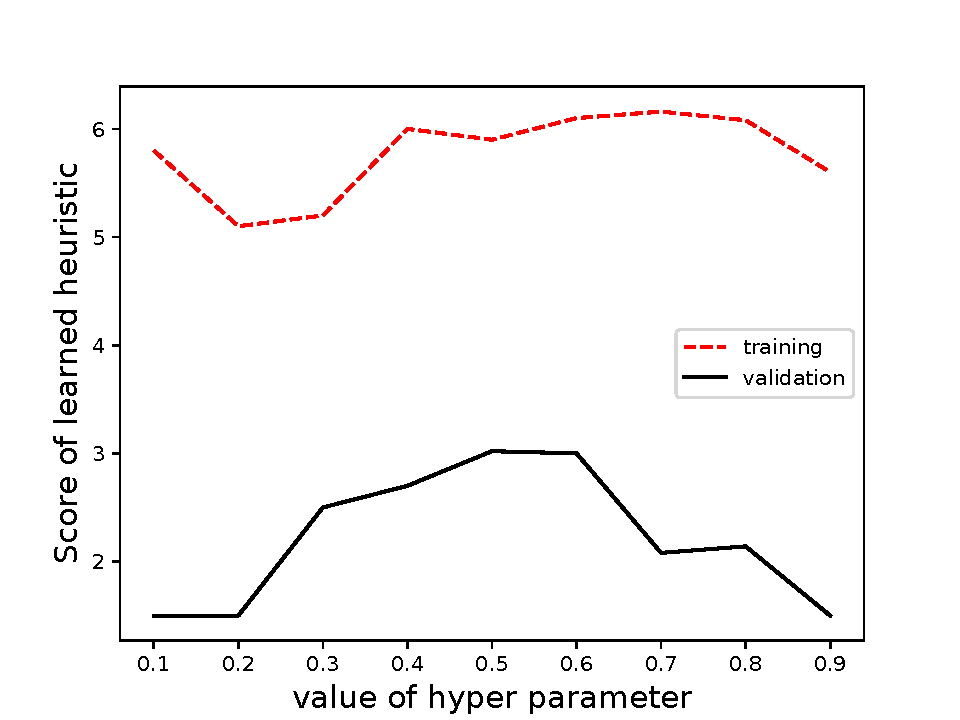
\includegraphics[width=6.3cm]{Graphick/figures/ctx_gamma.pdf}
	\caption{Object-sensitivity heuristic}
	\end{subfigure}
~\columnbreak

	\begin{subfigure}[t]{1.\columnwidth}
	\centering	
	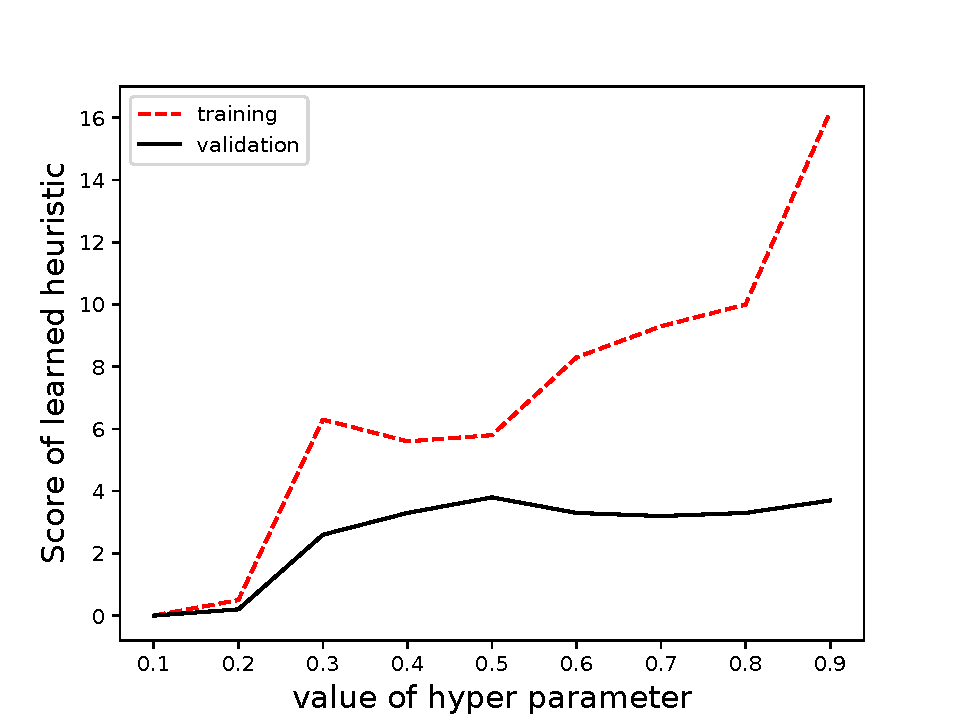
\includegraphics[width=6.3cm]{Graphick/figures/heap_gamma.pdf}
	\caption{Heap abstraction heuristic}
	\end{subfigure}
	\end{multicols}
	\caption{How score of learned heuristic changes over the value of $\hyper$.}
	\label{fig:gamma}
\end{figure}


\myparagraph{Choosing Hyper-Parameter $\hyper$}\label{sec:hyper_param}

Through our evaluation, we observed that the value of the hyper-parameter $\hyper$ plays an important role in the performance of the learned heuristic.
Figure~\ref{fig:gamma} depicts how performance of learned heuristics changes over the values of  $\hyper$.
The X-axis presents the value of $\hyper$ set to learn each heuristic, and
the Y-axis presents scores that we measured for performance of each heuristic $\heuristic_{\hyper}$ according to
${\sum_{P\in\vec{P}}\projproved(F_P(\heuristic_{\hyper}(G)))}\over{\sum_{P\in\vec{P}}
  \projcost(F_P(\heuristic_{\hyper}(G)))}$ where $\projcost$ denotes analysis time.
This score function presents the number of queries proved per second; thereby, more precise and scalable the analysis,
higher the score.
The red dotted and black solid lines present how the scores change over
the training programs $\vec{P}$ %(e.g., $\vec{P}$ = \{{\tt luindex,lusearch,antlr}\})
and the validation program, respectively.
For the training programs, the score of the learned heuristic increases as the higher $\hyper$ is given
because the heuristic becomes more fitted to the training programs.\footnote{It learned a bit bad heuristic when $\hyper$ is 0.9 in
  object-sensitivity heuristic because it is
difficult to generate specific features that satisfy such high precision
constraints; it eventually generates a general feature that include lots
of nodes.}
In our evaluation, both learned heuristics, however, perform the best on the validation program when $\hyper$ is 0.5;
thus, \OurCtx~in Table~\ref{tbl:contextAbstraction} and Table~\ref{tbl:heapAbstraction} corresponds to $\heuristic_{0.5}$.


%This occurs because the learned heuristics become overfitted to the training programs as the value of $\hyper$ increases;
%thus, simply increasing $\hyper$ is not an answer to achieve the best performance on validation and testing programs.







%\subsection{Learning Adequacy}

%\subsection{Insights from Generated Features}
\subsection{Learned Insights}

The learning algorithm generated 197 features in total for the object-sensitivity heuristic (68 features for 2-object-sensitivity, 29 for 2-type-sensitivity, and 100 features for 1-type-sensitivity). It generated 96 features for the heap abstraction heuristic.

\newcolumntype{P}[1]{>{\centering\arraybackslash}p{#1}}
\newcolumntype{M}[1]{>{\centering\arraybackslash}m{#1}}
\begin{figure}
\centering
\scriptsize
\setlength\extrarowheight{-1pt}
\begin{tabular}{|c|c|c| c | c | c |}
\toprule
\multicolumn{1}{|c}{}
                                                &                        & \multicolumn{1}{c|}{\textsf{Top 5 Features}} & \textsf{portion}
&\textsf{score} &
\multicolumn{1}{c|}{
\makecell{\textsf{Concretization}\\(Top 1)}
} \\ \midrule

\multirow{30}{*}{\rotatebox[origin=c]{90}{Object-Sensitivity Heuristic}}
& \multirow{10}{*}{\rotatebox[origin=c]{90}{1type}} &
\multirow{2}{*}{
\resizebox{0.40\columnwidth}{!}{
	\begin{tikzpicture}
	\node [block3,fill = gray] (n2) {{\tt\small [0,$\infty$],[61,$\infty$]}};
	\node [block3,right = 0.8cm of n2] (n3) {{\tt\small [46,$\infty$],[0,$\infty$]}};
	\path [line] (n2) -> (n3);
	\end{tikzpicture}
}
}
&\multirow{2}{*}{47\%} &\multirow{2}{*}{0.57}
                                        & \multirow{10}{*}{
		\resizebox{0.15\columnwidth}{!}{
			\begin{tikzpicture}
			\node [shape=circle,fill = gray,draw=black] (n1) {{\tt
                            n2}};
			\node [shape=circle,fill = gray,draw=black,left = 0.3cm
                        of n1] (n1left) {{\tt n1}};
			\node [shape=circle,fill = gray,draw=black,right = 0.3cm
                        of n1] (n1right) {{\tt n3}};
			\node [None,above = 0.7cm
                        of n1] (aboven1) {};
			\node [None,above = 0.7cm
                        of n1left] (aboven2) {};
			\node [None,above = 0.7cm
                        of n1right] (aboven3) {};
			\node [shape=circle,draw=black,below = 0.9cm
                        of n1] (n2) {{\tt n4}};
			\node [None,above left = 0.6 and 0.1cm
                        of n1] (n4) {};
			\node [None,right = 0.7cm
                        of n4] (n5) {};
			\node [None,above left = 0.7 and 0.5cm
                        of n2] (d1) {};
			\node [None, right = -0.1
                        of d1] (d2) {};
			\node [None, right = -0.1
                        of d2] (d3) {};
			\node [None, right = -0.1
                        of d3] (d4) {};
			\node [None, right = -0.1
                        of d4] (d5) {};
			\node [None, right = -0.1
                        of d5] (d6) {};
			\node [None, right = -0.1
                        of d6] (d7) {};
			\node [None, right = -0.1
                        of d7] (d8) {};
			\node [None, right = -0.1
                        of d8] (d9) {};
			\node [None, right = -0.1
                        of d9] (d10) {};
			\node [None, right = -0.1
                        of d10] (d11) {};
			\node [None, right = -0.1
                        of d11] (d12) {};
			\node [None, right = -0.1
                        of d12] (d13) {};		
			\path [line] (aboven1) -- (n1);
			\path [line] (aboven2) -- (n1left);
			\path [line] (aboven3) -- (n1right);
			\path [line] (n1left) -- (n2);
			\path [line] (n1right) -- (n2);
			\path [line] (n1) -- (n2);
			\path [line] (d1) -- (n2);
			\path [line] (d2) -- (n2);
			\path [line] (d3) -- (n2);
			\path [line] (d4) -- (n2);
			\path [line] (d5) -- (n2);
			\path [line] (d6) -- (n2);
			\path [line] (d7) -- (n2);
			\path [line] (d8) -- (n2);
			\path [line] (d9) -- (n2);
			\path [line] (d10) -- (n2);
			\path [line] (d11) -- (n2);
			\path [line] (d12) -- (n2);
			\path [line] (d13) -- (n2);
			\end{tikzpicture}
		}
}
                   \\
&&\multicolumn{1}{c|}{}&\multicolumn{1}{c|}{}  &\multicolumn{1}{c|}{}&\multicolumn{1}{c|}{}

\\
                                                &                        &
\multirow{2}{*}{
\resizebox{0.40\columnwidth}{!}{
	\begin{tikzpicture}
	\node [block3,fill = gray] (n2) {{\tt\small [0,$\infty$],[0,$\infty$]}};
	\node [block4,right = 0.8cm of n2] (n3) {{\tt\small [0,$\infty$],[117,$\infty$]}};
	\path [line] (n2) -> (n3);
	\end{tikzpicture}
}}
& \multirow{2}{*}{36\%} &\multirow{2}{*}{0.63}                                        &                                     \\
&&\multicolumn{1}{c|}{}&\multicolumn{1}{c|}{}  &\multicolumn{1}{c|}{}&\multicolumn{1}{c|}{}
\\
                                                &                        &
\multirow{2}{*}{
\resizebox{0.41\columnwidth}{!}{
	\begin{tikzpicture}
	\node [block4] (n2) {{\tt\small [0,$\infty$],[100,$\infty$]}};
	\node [block3,fill = gray,right = 0.8cm of n2] (n3) {{\tt\small [0,$\infty$],[29,$\infty$]}};
	\path [line] (n2) -> (n3);
	\end{tikzpicture}
}}
& \multirow{2}{*}{35\%} & \multirow{2}{*}{0.55}                                      &                                     \\
&&\multicolumn{1}{c|}{}&\multicolumn{1}{c|}{}  &\multicolumn{1}{c|}{}&\multicolumn{1}{c|}{}
\\
                                                &                        &
\multirow{2}{*}{
\resizebox{0.50\columnwidth}{!}{
	\begin{tikzpicture}
	\node [block4] (n2) {{\tt\small [0,$\infty$],[100,$\infty$]}};
	\node [block3,fill = gray,right = 0.3cm of n2] (n3) {{\tt\small [0,$\infty$],[0,$\infty$]}};
	\node [block4,right = 0.3cm of n3] (n4) {{\tt\small [0,$\infty$],[36,43]}};
	\path [line] (n2) -> (n3);
	\path [line] (n3) -> (n4);
	\end{tikzpicture}
}}
& \multirow{2}{*}{29\%} & \multirow{2}{*}{0.71}                                          &                                     \\
&&\multicolumn{1}{c|}{}&\multicolumn{1}{c|}{}  &\multicolumn{1}{c|}{}&\multicolumn{1}{c|}{}
\\


                                                &                        &
\multirow{2}{*}{
\resizebox{0.5\columnwidth}{!}{
	\begin{tikzpicture}
	\node [block4] (n2) {{\tt\small [0,$\infty$],[109,$\infty$]}};
	\node [block3,fill = gray,right = 0.3cm of n2] (n3) {{\tt\small [0,$\infty$],[0,$\infty$]}};
	\node [block4,right = 0.3cm of n3] (n4) {{\tt\small [171,$\infty$],[0,$\infty$]}};
	\path [line] (n2) -> (n3);
	\path [line] (n3) -> (n4);
	\end{tikzpicture}
}}
&\multirow{2}{*}{25\%}&\multirow{2}{*}{0.57}                                       &                                     \\
&&\multicolumn{1}{c|}{}&\multicolumn{1}{c|}{}  &\multicolumn{1}{c|}{}&\multicolumn{1}{c|}{}\\





\cline{2-6}
                                                & \multirow{10}{*}{\rotatebox[origin=c]{90}{2type}} &
\multirow{2}{*}{
\resizebox{0.40\columnwidth}{!}{
	\begin{tikzpicture}
	\node [block3] (n2) {{\tt\small [0,$\infty$],[36,39]}};
	\node [None ,above = 0.0cm of n2] (None) {};
	\node [block4 ,fill = gray,right = 0.8cm of n2] (n3) {{\tt\small [0,$\infty$],[73,75]}};
	\path [line] (n2) -> (n3);
	\end{tikzpicture}
}}
& \multirow{2}{*}{9\%}&\multirow{2}{*}{0.66}
                                                                                         & \multirow{10}{*}{
		\resizebox{0.15\columnwidth}{!}{
			\begin{tikzpicture}
			\node [shape=circle,fill = gray,draw=black] (n1) {{\tt
                            n2}};
			\node [shape=circle,draw=black,above = 0.5cm
                        of n1] (n0) {{\tt n1}};
			\node [None,below = 0.3cm
                        of n2] (bot) {};
			\node [None,right = 0.3cm
                        of n1] (n3) {};
			\node [None,above left = 0.4 and 0.5cm
                        of n0] (1d1) {};
			\node [None, right = -0.1
                        of 1d1] (1d2) {};
			\node [None, right = -0.1
                        of 1d2] (1d3) {};
			\node [None, right = -0.1
                        of 1d3] (1d4) {};
			\node [None, right = -0.1
                        of 1d4] (1d5) {};
			\node [None, right = -0.1
                        of 1d5] (1d6) {};
			\node [None, right = -0.1
                        of 1d6] (1d7) {};
			\node [None, right = -0.1
                        of 1d7] (1d8) {};
			\node [None, right = -0.1
                        of 1d8] (1d9) {};
			\node [None, right = -0.1
                        of 1d9] (1d10) {};
			\node [None, right = -0.1
                        of 1d10] (1d11) {};
			\node [None, right = -0.1
                        of 1d11] (1d12) {};
			\node [None, right = -0.1
                        of 1d12] (1d13) {};
			\node [None,below left = 0.3 and 0.7cm
                        of n0] (1e1) {};
			\node [None, right = -0.1
                        of 1e1] (1e2) {};
			\node [None, right = -0.1
                        of 1e2] (1e3) {};
			\node [None, right = -0.1
                        of 1e3] (1e4) {};
			\node [None, right = -0.1
                        of 1e4] (1e5) {};
			\node [None, right = -0.1
                        of 1e5] (1e6) {};
			\node [None, right = -0.1
                        of 1e6] (1e7) {};
			\node [None, right = -0.1
                        of 1e7] (1e8) {};
			\node [None, right = -0.1
                        of 1e8] (1e9) {};
			\node [None, right = -0.1
                        of 1e9] (1e10) {};
			\node [None, right = -0.1
                        of 1e10] (1e11) {};
			\node [None, right = -0.1
                        of 1e11] (1e12) {};
			\node [None, right = -0.1
                        of 1e12] (1e13) {};
			\node [None, right = -0.1
                        of 1e13] (1e14) {};
			\node [None, right = -0.1
                        of 1e14] (1e15) {};		
			\node [None,above left = 0.4 and 0.5cm
                        of n1] (d1) {};
			\node [None, right = -0.1
                        of d1] (d2) {};
			\node [None, right = -0.1
                        of d2] (d3) {};
			\node [None, right = -0.1
                        of d3] (d4) {};
			\node [None, right = -0.1
                        of d4] (d5) {};
			\node [None, right = -0.1
                        of d5] (d6) {};
			\node [None, right = -0.1
                        of d6] (d7) {};
			\node [None, right = -0.1
                        of d7] (d8) {};
			\node [None, right = -0.1
                        of d8] (d9) {};
			\node [None, right = -0.1
                        of d9] (d10) {};
			\node [None, right = -0.1
                        of d10] (d11) {};
			\node [None, right = -0.1
                        of d11] (d12) {};
			\node [None, right = -0.1
                        of d12] (d13) {};
			\node [None,below left = 0.5 and 0.7cm
                        of n1] (e1) {};
			\node [None, right = -0.1
                        of e1] (e2) {};
			\node [None, right = -0.1
                        of e2] (e3) {};
			\node [None, right = -0.1
                        of e3] (e4) {};
			\node [None, right = -0.1
                        of e4] (e5) {};
			\node [None, right = -0.1
                        of e5] (e6) {};
			\node [None, right = -0.1
                        of e6] (e7) {};
			\node [None, right = -0.1
                        of e7] (e8) {};
			\node [None, right = -0.1
                        of e8] (e9) {};
			\node [None, right = -0.1
                        of e9] (e10) {};
			\node [None, right = -0.1
                        of e10] (e11) {};
			\node [None, right = -0.1
                        of e11] (e12) {};
			\node [None, right = -0.1
                        of e12] (e13) {};
			\node [None, right = -0.1
                        of e13] (e14) {};
			\node [None, right = -0.1
                        of e14] (e15) {};			
%			\path [line] (n0) -- (1e1);
			\path [line] (n0) -- (1e2);
			\path [line] (n0) -- (1e3);
			\path [line] (n0) -- (1e4);
			\path [line] (n0) -- (1e5);
			\path [line] (n0) -- (1e6);
			\path [line] (n0) -- (1e7);
			\path [line] (n0) -- (1e8);
			\path [line] (n0) -- (1e9);
			\path [line] (n0) -- (1e10);
			\path [line] (n0) -- (1e11);
			\path [line] (n0) -- (1e12);
			\path [line] (n0) -- (1e13);
			\path [line] (n0) -- (1e14);
%			\path [line] (n0) -- (1e15);
			\path [line] (n0) -- (n1);
%			\path [line] (n1) -- (e1);
			\path [line] (n1) -- (e2);
			\path [line] (n1) -- (e3);
			\path [line] (n1) -- (e4);
			\path [line] (n1) -- (e5);
			\path [line] (n1) -- (e6);
			\path [line] (n1) -- (e7);
			\path [line] (n1) -- (e8);
			\path [line] (n1) -- (e9);
			\path [line] (n1) -- (e10);
			\path [line] (n1) -- (e11);
			\path [line] (n1) -- (e12);
			\path [line] (n1) -- (e13);
			\path [line] (n1) -- (e14);
%			\path [line] (n1) -- (e15);
			\end{tikzpicture}
		}
}                   \\
&&\multicolumn{1}{c|}{}&\multicolumn{1}{c|}{}  &\multicolumn{1}{c|}{}&\multicolumn{1}{c|}{}
\\
                                                &                        &
\multirow{2}{*}{
\resizebox{0.18\columnwidth}{!}{
	\begin{tikzpicture}
	\node [block4,fill = gray] (n2) {{\tt\small [105,155],[0,$\infty$]}};
	\end{tikzpicture}
}}
&\multirow{2}{*}{9\%}&\multirow{2}{*}{1} 
&                                     \\
&&\multicolumn{1}{c|}{}&\multicolumn{1}{c|}{}  &\multicolumn{1}{c|}{}&\multicolumn{1}{c|}{}
\\
                                                &                        &
\multirow{2}{*}{
\resizebox{0.5\columnwidth}{!}{
	\begin{tikzpicture}
	\node [block3] (n2) {{\tt\small [0,$\infty$],[0,61]}};
	\node [block4,fill = gray,right = 0.3cm of n2] (n3) {{\tt\small [60,76],[0,61]}};
	\node [block3,right = 0.3cm of n3] (n4) {{\tt\small [0,22],[0,$\infty$]}};
	\path [line] (n2) -> (n3);
	\path [line] (n3) -> (n4);
	\end{tikzpicture}
}}
& \multirow{2}{*}{9\%} &\multirow{2}{*}{0.5}                                          &                                     \\
&&\multicolumn{1}{c|}{}&\multicolumn{1}{c|}{}  &\multicolumn{1}{c|}{}&\multicolumn{1}{c|}{}
\\
                                                &                        &
\multirow{2}{*}{
\resizebox{0.5\columnwidth}{!}{
	\begin{tikzpicture}
	\node [block3] (n2) {{\tt\small [0,$\infty$],[29,61]}};
	\node [block4,fill = gray,right = 0.3cm of n2] (n3) {{\tt\small [171,228],[0,$\infty$]}};
	\node [block3,right = 0.3cm of n3] (n4) {{\tt\small [0,46],[0,$\infty$]}};
	\path [line] (n2) -> (n3);
	\path [line] (n3) -> (n4);
	\end{tikzpicture}
}}
&\multirow{2}{*}{4\%} &\multirow{2}{*}{1}                                       &                                     \\
&&\multicolumn{1}{c|}{}&\multicolumn{1}{c|}{}  &\multicolumn{1}{c|}{}&\multicolumn{1}{c|}{}
\\
                                                &                        &
\multirow{2}{*}{
\resizebox{0.18\columnwidth}{!}{
	\begin{tikzpicture}
	\node [block3,fill = gray] (n2) {{\tt\small [84,91],[0,$\infty$]}};
	\end{tikzpicture}
}}
& \multirow{2}{*}{4\%} & \multirow{2}{*}{0.5}                                      &                                     \\
&&\multicolumn{1}{c|}{}&\multicolumn{1}{c|}{}  &\multicolumn{1}{c|}{}&\multicolumn{1}{c|}{}
\\
\cline{2-6}
 & \multirow{10}{*}{\rotatebox[origin=c]{90}{2obj}}  &
\multirow{2}{*}{
\resizebox{0.17\columnwidth}{!}{
	\begin{tikzpicture}
	\node [block3,fill = gray] (n2) {{\tt\small [0,$\infty$],[53,61]}};
	\node [None ,above = 0.0cm of n2] (None) {};
	\end{tikzpicture}
}}
& \multirow{2}{*}{9\%} & \multirow{2}{*}{0.53}
& \multirow{10}{*}{
\resizebox{0.15\columnwidth}{!}{
			\begin{tikzpicture}
			\node [None] (n1) {};
			\node [shape=circle,fill=gray,draw=black,below = 0.9cm
                        of n1] (n2) {{\tt n1}};
			\node [None,right = 0.3cm
                        of n1] (n3) {};
			\node [None,above left = 0.7 and 0.5cm
                        of n2] (d1) {};
			\node [None, right = -0.1
                        of d1] (d2) {};
			\node [None, right = -0.1
                        of d2] (d3) {};
			\node [None, right = -0.1
                        of d3] (d4) {};
			\node [None, right = -0.1
                        of d4] (d5) {};
			\node [None, right = -0.1
                        of d5] (d6) {};
			\node [None, right = -0.1
                        of d6] (d7) {};
			\node [None, right = -0.1
                        of d7] (d8) {};
			\node [None, right = -0.1
                        of d8] (d9) {};
			\node [None, right = -0.1
                        of d9] (d10) {};
			\node [None, right = -0.1
                        of d10] (d11) {};
			\node [None, right = -0.1
                        of d11] (d12) {};
			\node [None, right = -0.1
                        of d12] (d13) {};
			\node [None,below left = 0.9 and 0.7cm
                        of n2] (e1) {};
			\node [None, right = -0.1
                        of e1] (e2) {};
			\node [None, right = -0.1
                        of e2] (e3) {};
			\node [None, right = -0.1
                        of e3] (e4) {};
			\node [None, right = -0.1
                        of e4] (e5) {};
			\node [None, right = -0.1
                        of e5] (e6) {};
			\node [None, right = -0.1
                        of e6] (e7) {};
			\node [None, right = -0.1
                        of e7] (e8) {};
			\node [None, right = -0.1
                        of e8] (e9) {};
			\node [None, right = -0.1
                        of e9] (e10) {};
			\node [None, right = -0.1
                        of e10] (e11) {};
			\node [None, right = -0.1
                        of e11] (e12) {};
			\node [None, right = -0.1
                        of e12] (e13) {};
			\node [None, right = -0.1
                        of e13] (e14) {};
			\node [None, right = -0.1
                        of e14] (e15) {};			
			\path [line] (n1) -- (n2);
%			\path [line] (n2) -- (e1);
			\path [line] (n2) -- (e2);
			\path [line] (n2) -- (e3);
			\path [line] (n2) -- (e4);
			\path [line] (n2) -- (e5);
			\path [line] (n2) -- (e6);
			\path [line] (n2) -- (e7);
			\path [line] (n2) -- (e8);
			\path [line] (n2) -- (e9);
			\path [line] (n2) -- (e10);
			\path [line] (n2) -- (e11);
			\path [line] (n2) -- (e12);
			\path [line] (n2) -- (e13);
			\path [line] (n2) -- (e14);
%			\path [line] (n2) -- (e15);
			\end{tikzpicture}
		}
}                   \\
&&\multicolumn{1}{c|}{}&\multicolumn{1}{c|}{}  &\multicolumn{1}{c|}{}&\multicolumn{1}{c|}{}
\\
                                                &
                                                                        &
\multirow{2}{*}{
\resizebox{0.17\columnwidth}{!}{
\begin{tikzpicture}
\node [block3,fill = gray] (n2) {{\tt\small [0,$\infty$],[24,25]}};
\end{tikzpicture}
}}
&\multirow{2}{*}{6\%} &\multirow{2}{*}{0.53}                                       &                                     \\
&&\multicolumn{1}{c|}{}&\multicolumn{1}{c|}{}  &\multicolumn{1}{c|}{}&\multicolumn{1}{c|}{}
\\
                                                &                        &
\multirow{2}{*}{\resizebox{0.5\columnwidth}{!}{
	\begin{tikzpicture}
	\node [block4,fill = gray] (n2) {{\tt\small [0,$\infty$],[0,7]}};
	\node [block3,right = 0.3cm of n2] (n3) {{\tt\small [9,11],[0,$\infty$]}};
	\node [block3,right = 0.3cm of n3] (n4) {{\tt\small [76,$\infty$],[0,$\infty$]}};
	\path [line] (n2) -> (n3);
	\path [line] (n3) -> (n4);
	\end{tikzpicture}
}}
&\multirow{2}{*}{2\%}&\multirow{2}{*}{0.82}                                        & \\
&&\multicolumn{1}{c|}{}&\multicolumn{1}{c|}{}  &\multicolumn{1}{c|}{}&\multicolumn{1}{c|}{}
\\

                                                &                        &
\multirow{2}{*}{\resizebox{0.5\columnwidth}{!}{
	\begin{tikzpicture}
	\node [block4] (n2) {{\tt\small [0,$\infty$],[43,$\infty$]}};
	\node [block3,fill = gray,right = 0.3cm of n2] (n3) {{\tt\small [0,$\infty$],[0,14]}};
	\node [block3,right = 0.3cm of n3] (n4) {{\tt\small [22,24],[0,$\infty$]}};
	\path [line] (n2) -> (n3);
	\path [line] (n3) -> (n4);
	\end{tikzpicture}
}}
&\multirow{2}{*}{1\%}&\multirow{2}{*}{0.63}                                        &                                     \\
&&\multicolumn{1}{c|}{}&\multicolumn{1}{c|}{}  &\multicolumn{1}{c|}{}&\multicolumn{1}{c|}{}
\\
                                                &
                                                                        &
\multirow{2}{*}{\resizebox{0.5\columnwidth}{!}{
	\begin{tikzpicture}
	\node [block4] (n2) {{\tt\small [0,$\infty$],[145,147]}};
	\node [block3,fill = gray,right = 0.3cm of n2] (n3) {{\tt\small [0,$\infty$],[0,$\infty$]}};
	\node [block3,right = 0.3cm of n3] (n4) {{\tt\small [0,46],[0,$\infty$]}};
	\path [line] (n2) -> (n3);
	\path [line] (n3) -> (n4);
	\end{tikzpicture}
}}                                                                                &\multirow{2}{*}{1\%}&\multirow{2}{*}{0.69}&                                     \\
&&\multicolumn{1}{c|}{}&\multicolumn{1}{c|}{}  &\multicolumn{1}{c|}{}&\multicolumn{1}{c|}{}
\\

%                                                &                        &
%\resizebox{0.45\columnwidth}{!}{
%	\begin{tikzpicture}
%	\node [block3,fill = gray] (n2) {{\tt\small [0,$\infty$],[0,3]}};
%	\node [block4,right = 0.8cm of n2] (n3) {{\tt\small [22,33],[0,$\infty$]}};
%	\path [line] (n2) -> (n3);
%	\end{tikzpicture}
%}                                       &                                     \\
 \midrule\midrule
\multicolumn{2}{|c|}{\multirow{10}{*}{
		\rotatebox[origin=c]{90}{\makecell{Heap Abstraction\\Heuristic}}}}        &
\multirow{2}{*}{\resizebox{0.5\columnwidth}{!}{
	\begin{tikzpicture}
	\node [block3,fill = gray] (n2) {{\tt\small [0,$\infty$],[0,3]}};
	\node [block4,right = 0.3cm of n2] (n3) {{\tt\small [48,$\infty$],[0,$\infty$]}};
	\node [block4,right = 0.3cm of n3] (n4) {{\tt\small [0,$\infty$],[140,$\infty$]}};
	\path [line] (n2) -> (n3);
	\path [line] (n3) -> (n4);
	\end{tikzpicture}
}}
& \multirow{2}{*}{35\%} &\multirow{2}{*}{0.61} 

& \multirow{10}{*}{
		\resizebox{0.15\columnwidth}{!}{
			\begin{tikzpicture}
			\node [shape=circle,fill = gray,draw=black] (n1) {{\tt
                            n1}};
			\node [shape=circle,draw=black,below = 0.6cm
                        of n1] (n2) {{\tt n2}};
			\node [shape=circle,draw=black,below = 0.6cm
                        of n2] (n4) {{\tt n3}};
			\node [None,right = 0.3cm
                        of n1] (n3) {};
			\node [None,above left = 0.5 and 0.5cm
                        of n2] (d1) {};
			\node [None, right = -0.1
                        of d1] (d2) {};
			\node [None, right = -0.1
                        of d2] (d3) {};
			\node [None, right = -0.1
                        of d3] (d4) {};
			\node [None, right = -0.1
                        of d4] (d5) {};
			\node [None, right = -0.1
                        of d5] (d6) {};
			\node [None, right = -0.1
                        of d6] (d7) {};
			\node [None, right = -0.1
                        of d7] (d8) {};
			\node [None, right = -0.1
                        of d8] (d9) {};
			\node [None, right = -0.1
                        of d9] (d10) {};
			\node [None, right = -0.1
                        of d10] (d11) {};
			\node [None, right = -0.1
                        of d11] (d12) {};
			\node [None, right = -0.1
                        of d12] (d13) {};
			\node [None,below left = 0.4 and 0.7cm
                        of n2] (e1) {};
			\node [None, right = -0.1
                        of e1] (e2) {};
			\node [None, right = -0.1
                        of e2] (e3) {};
			\node [None, right = -0.1
                        of e3] (e4) {};
			\node [None, right = -0.1
                        of e4] (e5) {};
			\node [None, right = -0.1
                        of e5] (e6) {};
			\node [None, right = -0.1
                        of e6] (e7) {};
			\node [None, right = -0.1
                        of e7] (e8) {};
			\node [None, right = -0.1
                        of e8] (e9) {};
			\node [None, right = -0.1
                        of e9] (e10) {};
			\node [None, right = -0.1
                        of e10] (e11) {};
			\node [None, right = -0.1
                        of e11] (e12) {};
			\node [None, right = -0.1
                        of e12] (e13) {};
			\node [None, right = -0.1
                        of e13] (e14) {};
			\node [None, right = -0.1
                        of e14] (e15) {};	
			\node [None,above left = 0.3 and 0.5cm
                        of n4] (1d1) {};
			\node [None, right = -0.1
                        of 1d1] (1d2) {};
			\node [None, right = -0.1
                        of 1d2] (1d3) {};
			\node [None, right = -0.1
                        of 1d3] (1d4) {};
			\node [None, right = -0.1
                        of 1d4] (1d5) {};
			\node [None, right = -0.1
                        of 1d5] (1d6) {};
			\node [None, right = -0.1
                        of 1d6] (1d7) {};
			\node [None, right = -0.1
                        of 1d7] (1d8) {};
			\node [None, right = -0.1
                        of 1d8] (1d9) {};
			\node [None, right = -0.1
                        of 1d9] (1d10) {};
			\node [None, right = -0.1
                        of 1d10] (1d11) {};
			\node [None, right = -0.1
                        of 1d11] (1d12) {};
			\node [None, right = -0.1
                        of 1d12] (1d13) {};
			\node [None,below left = 0.5 and 0.7cm
                        of n4] (1e1) {};
			\node [None, right = -0.1
                        of 1e1] (1e2) {};
			\node [None, right = -0.1
                        of 1e2] (1e3) {};
			\node [None, right = -0.1
                        of 1e3] (1e4) {};
			\node [None, right = -0.1
                        of 1e4] (1e5) {};
			\node [None, right = -0.1
                        of 1e5] (1e6) {};
			\node [None, right = -0.1
                        of 1e6] (1e7) {};
			\node [None, right = -0.1
                        of 1e7] (1e8) {};
			\node [None, right = -0.1
                        of 1e8] (1e9) {};
			\node [None, right = -0.1
                        of 1e9] (1e10) {};
			\node [None, right = -0.1
                        of 1e10] (1e11) {};
			\node [None, right = -0.1
                        of 1e11] (1e12) {};
			\node [None, right = -0.1
                        of 1e12] (1e13) {};
			\node [None, right = -0.1
                        of 1e13] (1e14) {};
			\node [None, right = -0.1
                        of 1e14] (1e15) {};				
			\path [line] (n1) -- (n2);
			\path [line] (n1) -- (n3);
			\path [line] (d1) -- (n2);
			\path [line] (d2) -- (n2);
			\path [line] (d3) -- (n2);
			\path [line] (d4) -- (n2);
			\path [line] (d5) -- (n2);
			\path [line] (d6) -- (n2);
			\path [line] (d7) -- (n2);
			\path [line] (d8) -- (n2);
			\path [line] (d9) -- (n2);
			\path [line] (d10) -- (n2);
			\path [line] (d11) -- (n2);
			\path [line] (d12) -- (n2);
			\path [line] (d13) -- (n2);
%			\path [line] (n2) -- (e1);
			\path [line] (n2) -- (e2);
			\path [line] (n2) -- (e3);
			\path [line] (n2) -- (e4);
			\path [line] (n2) -- (e5);
			\path [line] (n2) -- (e6);
			\path [line] (n2) -- (e7);
			\path [line] (n2) -- (e8);
			\path [line] (n2) -- (e9);
			\path [line] (n2) -- (e10);
			\path [line] (n2) -- (e11);
			\path [line] (n2) -- (e12);
			\path [line] (n2) -- (e13);
			\path [line] (n2) -- (e14);
%			\path [line] (n2) -- (e15);
			\path [line] (n2) -- (n4);
			\path [line] (1d1) -- (n4);
			\path [line] (1d2) -- (n4);
			\path [line] (1d3) -- (n4);
			\path [line] (1d4) -- (n4);
			\path [line] (1d5) -- (n4);
			\path [line] (1d6) -- (n4);
			\path [line] (1d7) -- (n4);
			\path [line] (1d8) -- (n4);
			\path [line] (1d9) -- (n4);
			\path [line] (1d10) -- (n4);
			\path [line] (1d11) -- (n4);
			\path [line] (1d12) -- (n4);
			\path [line] (1d13) -- (n4);
%			\path [line] (n4) -- (1e1);
			\path [line] (n4) -- (1e2);
			\path [line] (n4) -- (1e3);
			\path [line] (n4) -- (1e4);
			\path [line] (n4) -- (1e5);
			\path [line] (n4) -- (1e6);
			\path [line] (n4) -- (1e7);
			\path [line] (n4) -- (1e8);
			\path [line] (n4) -- (1e9);
			\path [line] (n4) -- (1e10);
			\path [line] (n4) -- (1e11);
			\path [line] (n4) -- (1e12);
			\path [line] (n4) -- (1e13);
			\path [line] (n4) -- (1e14);
%			\path [line] (n4) -- (1e15);
			\end{tikzpicture}
		}
}\\
\multicolumn{1}{|c}{}&\multicolumn{1}{c|}{}&\multicolumn{1}{c|}{}&\multicolumn{1}{c|}{}  &\multicolumn{1}{c|}{}&\multicolumn{1}{c|}{}
\\
\multicolumn{2}{|l|}{}                                                   &
\multirow{2}{*}{\resizebox{0.5\columnwidth}{!}{
	\begin{tikzpicture}
	\node [block3,fill = gray] (n2) {{\tt\small [0,12],[0,3]}};
	\node [block4,right = 0.3cm of n2] (n3) {{\tt\small [0,97],[0,$\infty$]}};
	\node [block4,right = 0.3cm of n3] (n4) {{\tt\small [0,$\infty$],[140,$\infty$]}};
	\path [line] (n2) -> (n3);
	\path [line] (n3) -> (n4);
	\end{tikzpicture}
}}
&\multirow{2}{*}{33\%}
&\multirow{2}{*}{0.53}                                      &                                     \\
\multicolumn{1}{|c}{}&\multicolumn{1}{c|}{}&\multicolumn{1}{c|}{}&\multicolumn{1}{c|}{}  &\multicolumn{1}{c|}{}&\multicolumn{1}{c|}{}
\\
\multicolumn{2}{|l|}{}                                                   &
\multirow{2}{*}{\resizebox{0.40\columnwidth}{!}{
	\begin{tikzpicture}
	\node [block4,fill = gray] (n3) {{\tt\small [38,$\infty$],[0,62]}};
	\node [block4,right = 0.8cm of n3] (n4) {{\tt\small [0,$\infty$],[236,$\infty$]}};
	\path [line] (n3) -> (n4);
	\end{tikzpicture}
}}
& \multirow{2}{*}{27\%} &\multirow{2}{*}{0.59}                                        &                                     \\
\multicolumn{1}{|c}{}&\multicolumn{1}{c|}{}&\multicolumn{1}{c|}{}&\multicolumn{1}{c|}{}  &\multicolumn{1}{c|}{}&\multicolumn{1}{c|}{}
\\
\multicolumn{2}{|l|}{}                                                   &
\multirow{2}{*}{\resizebox{0.40\columnwidth}{!}{
	\begin{tikzpicture}
	\node [block4,fill = gray] (n3) {{\tt\small [0,48],[0,62]}};
	\node [block4,right = 0.8cm of n3] (n4) {{\tt\small [72,84],[0,$\infty$]}};
	\path [line] (n3) -> (n4);
	\end{tikzpicture}
}}
& \multirow{2}{*}{24\%} & \multirow{2}{*}{0.53} 
                                         &\\
\multicolumn{1}{|c}{}&\multicolumn{1}{c|}{}&\multicolumn{1}{c|}{}&\multicolumn{1}{c|}{}  &\multicolumn{1}{c|}{}&\multicolumn{1}{c|}{}
\\
\multicolumn{2}{|l|}{}                                                   &
\multirow{2}{*}{\resizebox{0.5\columnwidth}{!}{
	\begin{tikzpicture}
	\node [block3,fill = gray] (n2) {{\tt\small [0,24],[0,$\infty$]}};
	\node [block4,right = 0.3cm of n2] (n3) {{\tt\small [21,$\infty$],[140,$\infty$]}};
	\node [block4,right = 0.3cm of n3] (n4) {{\tt\small [0,97],[0,$\infty$]}};
	\path [line] (n2) -> (n3);
	\path [line] (n3) -> (n4);
	\end{tikzpicture}
}}
& \multirow{2}{*}{22\%} & \multirow{2}{*}{0.53} 
                                         &                                     \\
\multicolumn{1}{|c}{}&\multicolumn{1}{c|}{}&\multicolumn{1}{c|}{}&\multicolumn{1}{c|}{}  &\multicolumn{1}{c|}{}&\multicolumn{1}{c|}{}
\\
%\multicolumn{2}{|l|}{}                                                   &
%\resizebox{0.45\columnwidth}{!}{
%	\begin{tikzpicture}
%	\node [block3,fill = gray] (n2) {{\tt\small [0,48],[0,$\infty$]}};
%	\node [block4,right = 0.8cm of n2] (n3) {{\tt\small [72,84],[0,$\infty$]}};
%
%	\path [line] (n2) -> (n3);
%	\end{tikzpicture}
%}                                         &                                     \\
\bottomrule
\end{tabular}
\caption{Top-5 features learned by our technique, and concrete nodes implied by the top-1 feature.
%Gray colored abstract nodes in the features correspond to the target nodes and others are predecessors or successors.
%Gray colored nodes in the column \textsf{Concretization} are precision-critical nodes which are selected by the first features; 
%other nodes are predecessors or successors that make the gray colored nodes satisfy the features.
}
\label{fig:features}
\end{figure}



%%% Local Variables:
%%% mode: latex
%%% TeX-master: "paper"
%%% End:


\myparagraph{Top-5 Features}
Figure~\ref{fig:features} describes the most informative features generated by our technique for each abstraction degree and their concretization in the given graphs.
The second column \textsf{Top 5 Features}, in decreasing order of \textsf{portion}, presents top 5 features which have the greatest number of precision-critical nodes satisfying the features with scores above 0.5.
For example, the first feature in 1type contains 47\% nodes of the total precision-critical nodes which are to be applied 1-type-sensitivity,
and has a score of 0.57.
If a feature is too general (e.g., $(\epsilon, ([0,\infty],[0,\infty]), \epsilon)$), it is excluded even with a large portion (e.g., 100\%)
because its score is under 0.5.
Similarly, if a feature is too specific, it is also excluded because it includes a small number of precision-critical nodes even with a good score.
For the features, the gray colored abstract nodes correspond to the target one $\hat{n}$ in each feature
(e.g., $(\seq{\myhat{p}_0,\myhat{p}_1,\dots,\myhat{p}_q}, \myhat{n}, \seq{\myhat{s}_0,\myhat{s}_1,\dots,\myhat{s}_r}) \in \Feature$).
Other nodes are predecessors or successors of the target abstract nodes (e.g., $\myhat{p}_0$, $\myhat{s}_0$, and $\myhat{s}_1$).
For each feature, we show the number of satisfying nodes over the total precision-critical nodes in the given graphs (\textsf{portion}) and the scores (\textsf{score}).
The right most column, \textsf{Concretization}, illustrates the visualized concretization for each first feature in \textsf{Top 5 Features} column,
%in the real graphs over the training programs, where the gray colored nodes correspond to the target nodes of the first feature.
where the gray colored nodes correspond to the target abstract nodes of the first feature.
For space reasons, we draw each node to have at most 13 incoming and outgoing edges although it can have more than 13 edges.


\begin{table}[]
\setlength\extrarowheight{-1pt}
\caption{Performance of our manually-designed graph-based heap abstraction heuristic for FPG}
\label{tbl:principle}
\centering
\footnotesize
\begin{tabular}{@{}clrr | clrr@{}}
\toprule
benchmarks               & \multicolumn{1}{c}{} & \multicolumn{1}{c}{alarms} & \multicolumn{1}{c|}{time(s)} & benchmarks                & \multicolumn{1}{c}{} & \multicolumn{1}{c}{alarms} & \multicolumn{1}{c}{time(s)} \\ \midrule
\multirow{2}{*}{luindex} & \Principle              & 374                        & 29(+29)                         & \multirow{2}{*}{lusearch} & \Principle            & 388                        & 33(+31)                        \\
                         % & \OurHeap            & 358                        & 23                          &                           & \OurHeap              & 372                        & 21                          \\
                         & \AllocBased          & 358                        & 5,475                       &                           & \AllocBased          & -                          & $>$10,800        \\\midrule
\multirow{2}{*}{antlr}   & \Principle              & 478                        & 44(+47)                        & \multirow{2}{*}{pmd$_{m}$}      & \Principle            & 886                        & 83(+65)                          \\
                         % & \OurHeap            & 463                        & 49                          &                           & \OurHeap              & 871                        & 48                          \\
                         & \AllocBased          & 463                        & 5,241                       &                           & \AllocBased          & 871                        & 9,146                       \\\midrule
\multirow{2}{*}{fop}     & \Principle            & 391                        & 41(+46)                          & \multirow{2}{*}{xalan}    & \Principle            & 548                        & 841(+85)                         \\
                         % & \OurHeap              & 376                        & 30                          &                           & \OurHeap              & 539                        & 489                         \\
                         & \AllocBased          & -                          & $>$10,800        &                           & \AllocBased          & -                          & $>$10,800        \\ \bottomrule
\end{tabular}
\end{table}


\myparagraph{Insights}

The generated features during the learning process provide hints on designing analysis heuristics from the graphs.
For example, we investigated the features of the heap abstraction heuristic in Figure~\ref{fig:features} and found two commonalities in them.
First,  the features have the form of $(\epsilon,\hat{n}, \hat{\vec{s}})$ where $\hat{\vec{s}}$ is not $\epsilon$,
which implies that we should consider successors more than predecessors when designing heap abstraction heuristics from points-to graph.
The second commonality is that $\hat{\vec{s}}$ or $\hat{n}$ tends to include an abstract
node $\aNode$ that presents nodes with lots of outgoing edges, i.e., $\aNode =
(itv,[b,\infty])$ where the number $b$ is about $3\%$ of the total nodes in a graph of a training program.
From these observations, we manually designed a graph-based heap abstraction heuristic which
assigns allocation-site based heap abstraction to the target nodes
if at least $3\%$ of the total nodes in FPG belong to either the target node or its successor nodes
(i.e. $\heuristic = \seq{\{ (\epsilon,([0,\infty],[b',\infty]),\epsilon)
	,(\epsilon,\top,\seq{([0,\infty],[b',\infty])})
	,(\epsilon,\top,\seq{\top,([0,\infty],[b',\infty])})
	,\dots
	\}
}$ where $\top$ equals to the most general one $([0,\infty],[0,\infty])$ and $b'$ is 3\% of the total nodes in the given graph).
Otherwise, the heuristic assigns type-based heap abstraction to the others.
%where $\top$ equals to the most general abstract node $([0,\infty],[0,\infty])$, and $b$ equals to 3\% of the total nodes in the given graph).
Table~\ref{tbl:principle} demonstrates the performance of the manually-crafted heuristic.
In comparison to \AllocBased, it reduces about 99\% of analysis cost while producing only 2\% more alarms.
%Compared to the baseline heuristic~\AllocBased,



Intuitively, the nodes with lots of successors in FPG should be analyzed precisely because merging the objects with others would produce lots of spurious analysis results.
For example, if there exists an object with lots of field objects which we want to merge with another one with a few field objects,
it eventually produces lots of spurious results stating that the both heaps can have lots of field objects.
%Such insight is related with that of \Mahjong~which merges the two objects if they have the same types of successors because,
%statically, an object having lots of successors is hard to have exactly the same types of successors with other objects.
Such insight is related with that of \Mahjong~which merges the objects if their successors have the same type;
statistically, if an object has lots of successors, there hardly exist the other objects with exactly the same types of successors.
Surprisingly, it is easy to find such insight through the features generated by our technique.
Note that this insight is general as it is not dependent to Java programs.
For example, when analyzing a C program, it is a required task not to merge such heaps with others as it would produce lots of spurious results.

%\textcolor{black}{
%\myparagraph{Graphick vs Scaler}
%Interestingly, Figure~\ref{fig:features} shows that the insight learned statistically can differ from the logic-based insight
%through the difference between \OurCtx~and \Scaler~in deciding which nodes to analyze more precisely.
Interestingly, Figure~\ref{fig:features} also shows the difference between the statistically-learned insight behind \OurCtx~and the logical insight behind \Scaler~in deciding which nodes to analyze more precisely.
Based on the logical insight, \Scaler~relies heavily on the number of incoming edges
as that number in the object allocation graph indicates %{\color{red}{
how many contexts will be constructed in object sensitivity.%}}
~\ourtool, however, treats the number of neighbor nodes' outgoing edges more importantly, as shown in Figure 6.
Such differences result in the performance gap between the two object-sensitivity heuristics.
%which shows better performance in both precision and scalability than the logic-based insight.
%}

%\textcolor{red}{
\myparagraph{Generality of learned heuristic}
We found the learned heuristic for object sensitivity is general to the hybrid-context sensitivity~\cite{KastrinisS13a}. Table~\ref{tbl:hybrid} presents the performance of the conventional 2-hybrid-context sensitivity (\twosobjH) and
2-hybrid-context sensitivity with the learned heuristic (\ourtool) used in Section~\ref{sec:comparescaler}.
%when using 6 DaCapo benchmark programs as testing programs.
The table shows that \ourtool~is also cost-effective compared to \twosobjH. For example, on a test program bloat,
\ourtool~produces only 22 more alarms while reducing about 90\% of analysis costs.
%}



\begin{table}[]
\setlength\extrarowheight{-1pt}
\caption{Performance comparison between conventional 2-hybrid-context-sensitivity (\twosobjH) and 2-hybrid-context-sensitivity with our learned heuristic for 2-object-sensitivity (\ourtool).}
\label{tbl:hybrid}
\centering\footnotesize
\begin{tabular}{@{}clrrrrrr@{}}
\toprule
                          & \multicolumn{1}{c}{} & \multicolumn{1}{c}{pmd$_m$} & \multicolumn{1}{c}{chart} & \multicolumn{1}{c}{eclipse} & \multicolumn{1}{c}{xalan} & \multicolumn{1}{c}{fop} & \multicolumn{1}{c}{bloat}  \\ \midrule
\multirow{2}{*}{\ourtool} & \#may-fail casts     & 220                      & 867                       & 2,880                        & 479                       & 1,408                    & 1,147                      \\
                          & analysis time (s)    & 45+(78)                  & 83(+76)                   & 1,426(+105)                  & 185(+57)                  & 245(+85)                & 215(+30)                  \\ \midrule
\multirow{2}{*}{\twosobjH}    & \#may-fail casts     & 220                      & 757                       & -                       & 447                          &  1,295                       & 1,125                          \\
                          & analysis time (s)    & 42                       & 195                       & $>$ 10,800                            & 428                          & 818                        & 2,238                           \\
%\midrule
%\multirow{2}{*}{\Insens}   & \#may-fail casts     & 679                      & 1,810                      & 4190                        & 1,182                      & 2,458                    & 1,924                      \\
%                          & analysis time (s)    & 23                       & 48                        & 91                          & 37                        & 53                      & 20                        \\
\bottomrule
\end{tabular}
\end{table}




%%% Local Variables:
%%% mode: latex
%%% TeX-master: "paper"
%%% End:

\section{Related Work}\label{sec:related}

Points-to analysis has a large body of past
literature\cite{Lhotak2006,Smaragdakis2015,hind2001pointer,Lhotak2008,Might2010,
 liang1999efficient,wilson1995efficient, liang2005evaluating, chatterjee1999relevant, Whaley2004, Shivers1988,Sharir1981, Milanova2005,Milanova2002, Smaragdakis2011, kastrinis2013hybrid}. Below, we discuss prior works that are closely related to
ours.

% been widely studied in past literature\cite{Lhotak2006,Smaragdakis2015,hind2001pointer,Lhotak2008,Might2010,
% liang1999efficient,wilson1995efficient, liang2005evaluating, chatterjee1999relevant, Whaley2004, Shivers1988,Sharir1981, Milanova2005,Milanova2002, Smaragdakis2011, kastrinis2013hybrid}.
% In this section, we discuss how this work contributes to context sensitive points-to anlaysis.

\subsection{Context-Sensitive Analysis} To our knowledge, all
existing techniques for context-sensitive analyses
(e.g.~\cite{Sharir1981,Milanova2002,Shivers1988,
  Whaley2004,Milanova2005,Smaragdakis2011, Khedker2008,
  Karkare2007,kastrinis2013hybrid,WeiR15,Smaragdakis2014,JeJeChOh17,Oh2014,TanLX16,PadhyeK13})
suffer from the problem we tackle in this paper. All of those
techniques update the calling contexts at every call-site and
therefore may lose important context elements when $k$-limiting is used.  For example,
techniques for varying context depths
adaptively~\cite{WeiR15,JeJeChOh17,Oh2014, Smaragdakis2014} have proven
their effectiveness for tuning the performance of context-sensitivity.  However,
the primary goal of these techniques is to selectively analyze methods
with appropriate $k$ values, rather than to be selective in context
construction.

% , instead of blindly applying $k$-context depth for all program
% parts and waste resources, making good prediction models that assign
% promising context depth for each method
% invocation. \citet{Smaragdakis2014} uses a manually-designed
% heuristic to identify ``break-even points'' of context sensitivity
% with pre-analysis, and then the main analysis selectively applies
% context-sensitivity with the prediction. \citet{JeJeChOh17}
% introduced a disjunctive model and a learning algorithm to infer
% such heuristics automatically from codebase. However, as far as
% those techniques rely on conventional $k$-limited
% context-sensitivity at their core, they suffer from the same problem
% that our paper concerns.

The technique, called \Bean, by~\citet{TanLX16} is similar to ours in
that it aims to improve precision of $k$-object-sensitive points-to
analysis without increasing $k$. The idea is to identify ``redundant''
context elements by running a pre-analysis and building a so-called
object allocation graph. An object allocation graph is analogous to a
call-graph in call-site-sensitivity and captures how context strings
are generated during an object-sensitive analysis. The technique
identifies redundant nodes in the graph, which can be removed without
reducing the number of distinct contexts; in fact, this technique
guarantees to result same or more distinct contexts than conventional
analysis with same $k$. The redundant nodes are excluded when
selecting heap contexts for an object. The main focus of \Bean~is in
choosing good heap contexts and therefore it still suffers from the
core problem we tackle in this paper; that is, \Bean~always append the
last context element to the parent context on method calls (i.e. it
uses the last rule in Figure~\ref{fig:baseline-rules}, not
Figure~\ref{fig:tunneling-rules}). As the result, when $k=1$ for
example, \Bean~analyzes every method under the same calling context as
the ordinary $1$-object-sensitive analysis. The goal of context
tunneling is to mitigate this problem.

Merging equivalent contexts~\cite{Xu2008} or abstract heaps~\cite{Tan2017} also have been studied to
increase scalability of context-sensitive points-to analysis. \citet{Xu2008} first defines a fine-grained
notion of context equivalence that guarantees to increase scalability without losing original analysis's
precision, which is $\infty$-context-sensitivity. Based on the equivalence, the paper introduces its abstracted
version to extend scalability even further at the cost of precision. \citet{Tan2017} merges two
abstract heaps if their fields-points-to-graphs indicate that any field access sequence (i.e.,
$o.f.g.\cdots .h$) ends up with same typed objects for two graphs. This approach demonstrated that it brings
little or no negative impact on precision but scales deep context
sensitive analysis.

% \citet{WeiR15} suggest a technique that choose a context from multiple kinds of context for each method to
% achieve precision. Such paramter share same goal of ours, but our technique uses a single kind of
% context to improve precision.


% Full context string approaches~\cite{Khedker2008, Karkare2007} has been used for a limited classes of data
% flow analysis problems for instance bit-vector problems. Naturally, various heuristics such as replacing
% consecutive context elements with the representative one~\cite{Khedker2008} or limiting occurrences of same
% context element~\cite{Karkare2007} have been proposed in order to mitigate possibly infinite length of call
% string thus poor scalability.


\subsection{Parametric and Data-Driven Program Analysis}

Our work presents a new instance of parametric program analysis.
Previously, parametric program analyses have been used for
context-sensitivity~\cite{Tan2017,Oh2014, JeJeChOh17, Liang2011learning, Zhang2014,Liang2011}, flow-sensitivity~\cite{Oh2015}, variable clustering for
relational analysis~\cite{Heo2016learning}, and widening
thresholds~\cite{cha2016learning}.
Typically, the goal of these analyses is to find a parameter which
is as scalable as possible while sacrificing as little precision as possible.
For example,
\citet{Oh2015,Oh2014,Smaragdakis2014, JeJeChOh17, Liang2011learning}
sacrifice the precision of full flow- or context-sensitivity to obtain
tractable scalability.
\citet{Heo2016learning} compromises the full precision of relational
analysis and cluster variables whose relationships should be kept
during analysis.
\citet{Hassanshahi2017} and \citet{Tan2017} aim to find appropriate heap
abstraction that scales well without losing precision too much.
In this paper, we propose a new knob, called context tunneling, which
is able to improve both precision and scalability of the conventional
context-sensitive analysis.

% Context tunneling is a unique knob to control both scalability
% and precision in context sensitive points to analysis. In parametric program analysis, analyzers are
% equipped with parameters and achieve cost effective analysis with suitable parameters.
% Most of the existing parameters in program
% analysis are designed to achieve scalability
% by sacrificing precision\cite{Oh2014,JeJeChOh17,Oh2015,Heo2016learning,cha2016learning}.
% \citet{Oh2015,Oh2014,Smaragdakis2014, Liang2011learning} use parameter that choose methods that should be analyzed
% context sensitively, \citet{JeJeChOh17} use parameter that assign context depth (0$\sim$k)for each method and
% parameters in \citet{Heo2016learning} cluster variables that analyzer should track the relations.
% \citet{Hassanshahi2017} use depth of heap contexts as a knob and the goal is to find appropriate heap
% context depth to each heap alloation site.
%  In such parameters, the goal of parameteric anlaysis is to find a parameter which
% are as scalable as possible while sacrificing precision as little as possible. Parameter in context
% tunneling, however, has different property that it is designed to achieve precision while not sacrificing
% scalability.

% \citet{Liang2011learning} defined the notion of minimal abstraction and suggested an algorithm to find the minimal
% abstractions for context-sensitivity in points-to analysis. However,
% the algorithm cannot be used for learning a program analysis
% heuristic.
% \citet{Zhang2014} proposed a CEGAR-based
% algorithm that learns a parameter for context-sensitive points-to analysis for Java. Both
% \citet{Liang2011learning} and \citet{Zhang2014} assume that abstractions are ordered with respect to
% precision like \citet{JeJeChOh17} while abstractions in context tunneling are not.


From the perspective of data-driven program analysis, our work
presents a new learning algorithm for disjunctive model that is
applicable even when the
underlying analysis is not monotone with respect to the parameter
space.
Recently, data-driven approaches to program analysis have been
popular to address the challenge of generating program-analysis
heuristics~\cite{JeJeChOh17,Oh2015,ChOhHeYa17,Heo2016learning,heo2016unsound,WeiR15}.
% Prior data-driven approaches in parametric program analysis are
% unable to learn suitable parameters in context tunneling. Data-driven program analysis aims to generate good
% program analysis heuristics automatically from
% codebase~\cite{JeJeChOh17,Oh2015,ChOhHeYa17,Heo2016learning,heo2016unsound,WeiR15}, and our work lies in
% this line of research.
In particular, \citet{JeJeChOh17} recently proposed an algorithm with
disjunctive model based on boolean formulas and used the model to
learn a heuristic to determine appropriate context depths for each
method. This algorithm drastically reduces the search space by
exploiting the monotonicity of the analysis (i.e. applying deeper context-sensitivity will never decrease precision). Our approach is based on the
disjunctive model proposed by~\cite{JeJeChOh17} but uses a
different, non-greedy algorithm for learning context tunneling
heuristics.
The learning algorithm by~\citet{Oh2015} is applicable to non-monotone
analyses, but its applicability is limited to analysis heuristics
based on the linear combination of input features.
\citet{ChOhHeYa17} solves an orthogonal problem, automatic
generation features for learning heuristics, where feature programs
are generated by running a program reducer and get abstracted to
features represented by abstract data-flow graphs. However, it remains
to be seen whether the technique is applicable beyond intraprocedural
settings.


% proposed an algorithm based on the simple linear
% combination of features and Bayesian optimization.
% learning strategy that use Bayesian optimization technique to
% learn parameters that use linear model.
% However, learning algorithms which learn linear combination do not
% work in our setting as we use different model\cite{Oh2015,Heo2016learning,heo2016unsound,cha2016learning}.
% \citet{JeJeChOh17} propose algorithms to learn parameter that assign appropriate context depth for each
% method. The algorithm drastically reduce search space by exploiting a property that applying deeper context
% sensitivity to methods do not lose precision. Although \citet{JeJeChOh17} use same model with ours, the
% algorithm is inappropriate to
% learn parameters in context tunneling as applying tunneling to methods may lose or gain precision.
% \citet{Liang2011learning} defines minimal abstraction and suggested an algorithm to finds the minimal
% abstractions of context-sensitivity in points-to analysis. \citet{Zhang2014} proposed a CEGAR-based
% algorithm that learns a parameter for context-sensitive points-to analysis for Java. Both
% \citet{Liang2011learning} and \citet{Zhang2014} assume that abstractions are ordered with respect to
% precision like \citet{JeJeChOh17} while abstractions in context tunneling are not.



%\myparagraph{Parametric program analysis}






% \myparagraph{Demand-driven Program Analysis}
% As we aim to analyze all queries in target programs, our approach differs from existing work on
% demand-driven program analysis~\cite{Guyer2003,
% Sridharan2006, Sridharan2005}. \citet{Yan2011} proposed demand-driven
% approach that improve scalability in CFL-reachability analysis. It achieves scalability by summarizing procedural reachability for frequently used methods
% during analysis and apply the summaries when CFL-reachability needs to enter the methods.
% % \citet{Allen2015} combine type analysis with points-to analysis for library codes to approximate behaviors of appli
%cations that use the libraries.
% \citet{Xu2009} improve performance of CFL-reachability analysis by using pre-analysis that compute
% must-not-alias information. Main analysis use pre-calculated information to prune out infeasible paths.


\begin{comment}
\begin{itemize}
\item{\citet{Hassanshahi2017} use selective object-sensitivity as a knob and the goal is to find appropriate heap context depth to each heap alloation site, and \citet{Hassanshahi2017} employ pre-analysis to identify program parts. -O}
\item{\citet{Yan2011} proposed demand-driven approach that improve scalability in CFL-reachability analysis.
\cite{Yan2011} achieve analysis scalability by summarizing procedural reachability for heavily used methods
during analysis and apply the summary when CFL-reachability needs to enter the methods. O}
\item{\citet{Xu2009} improve preformance of CFL-reachability analysis by using pre-analysis that compute
must-not-alias information. Main analysis use pre-calculated information to prune out infeasible paths. -O}
\item{\citet{Hassanshahi2017} use selective object-sensitivity as a knob and the goal is to find appropriate heap context depth to each heap alloation site, and \citet{Hassanshahi2017} employ pre-analysis to identify program parts. -O}
\item{\cite{Allen2015} combine type analysis with points to analysis for library codes to approximate behaviors of applications that use the libraries. O}

\item{To improve precision, \citet{Khedker2012} combined points-to anlaysis with liveness analysis resulting
precision improvement. X}
\item{\cite{Avots2005} states that pointer analysis can help bug detector for C by reducing overhead.X}
\item{\citet{Lam2005} propose hybrid pointer alias analysis that apply precise analysis for some parts
while  the other parts are being analyzed imprecisely. \cite{Lam2005} also introduce an unsound assumption
to reduce false positives and achieve scalability. X}
\item{\cite{Livshits2003}X}
\item{\cite{bodden2008object}}
\end{itemize}
\end{comment}
%\cite{Yan2011, Xu2009, Lam2005, Hassanshahi2017, Dietrich2015, Allen2015, Khedker2012, Avots2005, Livshits2003, bodden2008object}

%%%% Local Variables:
%%%% mode: latex
%%%% TeX-master: "paper"
%%%% End:

\section{Conclusion and Future Work}
%We showed that context tunneling is a promising way to gain both precision and scalability in $k$-limited context sensitive points to analysis. We also propose data-driven approach to automatically learn context tunneling heuristics. We have implemented our approach in Doop, and learn context tunneling heuristics for representative contexts in Java: selective hybrid object-sensitivity, object-sensitivity, type-sensitivity, and call-site sensitivity. Experimental results show that our approach achieve an extraordinary balance between precision and scalability. We believe that context tunneling is a big step forward in $k$-limited context sensitive points-to analysis. It is an effective technique that will rescue many key context elements resulting incredible analysis quality.

Developing a precise and scalable context-sensitive analysis
is a major challenge in program analysis research.  
This paper
demonstrates that we can effectively address this challenge by
applying context tunneling, which carefully maintains the
{\em $k$ most important} context elements, as opposed to the
traditional approaches that simply maintain the {\em $k$
  most recent} ones. 
Experimental results with four flavors of context-sensitivity show
that the new approach improves the state-of-the-art
points-to analyses remarkably in both
precision and scalability.
% However, as choosing
% important context elements is nontrivial, using an automated technique
% is essential for achieving effective context tunneling in practice.
To achieve this, we developed a new machine-learning algorithm specialized for generating
context-tunneling heuristics automatically from a dataset of programs.

We believe that the use of context tunneling is not limited
to points-to analysis for Java. As future work, we plan to apply
context tunneling to static analysis
for dynamic languages or control-flow analysis for functional
languages, where deeper context-sensitivity (e.g., $k > 5$) is known to be
greatly
beneficial~\cite{park_et_al:LIPIcs:2015:5245,Kashyap2014}.
Our conjecture is that the same (or even higher) precision can be obtained with smaller
$k$ values if they use context tunneling. 



% We have presented a new axis of parameterizing $k$-limited context sensitive points-to
% analysis, namely context tunneling heuristic, to improve precision and scalability.
% The key idea is ignoring worthless contexts while inheriting key contexts when methods
% are invoked. We use machine learning technique to automatically obtain classifiers who
% decides where to apply context tunneling. We applied the technique to well-known
% context sensitivities on top of Doop Java points-to analysis framework. Our
% experiments with these instances and benchmarks of DaCapo suite show that context
% tunneling makes $1$-context-sensitive analyses to have precision of deeper equivalents
% and performance of baselines.
%%% Local Variables:
%%% mode: latex
%%% TeX-master: "paper"
%%% End:

\appendix
%\section{Notations}\label{sec:max}
%The function $\MaxIn(G_\vec{P})$ returns the maximum number $max\in\mbn$ of
%incoming edges of a node in the graphs that $max$ satisfies:
%%\[
%%\begin{array}{c}
%\begin{enumerate}
%\item %There exists a node $n$ that have $max$ incoming edges:\\
%$max$ is a node's incoming edges:
%$\exists P\in\vec{P}. (N,E) =
%  G_\vec{P}(P) \land \exists n\in N. |\{n' \mid (n',n)\in E\}| = max$
%\item The node has equal or more number of
%incomingedges than the others: \\
%$\forall P \in \vec{P}. (N,E) = G_\vec{P}(P) \land \forall n\in N. |\{n' \mid (n',n)\in E
%\}| \le max$
%\end{enumerate}
%%\end{array}
%%\]
%On the other hand, $\MaxOut(G_\vec{P})$ returns the maximum number $max\in\mbn$ of
%outgoing edge of a node in the graphs:
%\begin{enumerate}
%\item $max$ is a node's outgoing edges: $\exists P\in\vec{P}. (N,E) = G_\vec{P}(P) \land \exists n\in N. |\{n' \mid (n,n')\in E
%\}| = max$
%\item The node has equal or more number of
%incomingedges than the others: \\
%$\forall P \in \vec{P}. (N,E) = G_\vec{P}(P) \land \forall n\in N. |\{n' \mid (n,n')\in E
%\}| \le max$
%\end{enumerate}

% \[
% Incoming(n,G) = |\{n' \mid (n',n)\in E \land G = (N,E) \}|
% \]
% \[
% Outgoing(n,G) = |\{n' \mid (n,n')\in E \land G = (N,E) \}|
% \]
% \[
% \forall n \in G' \in G_\vec{P}. Incoming(n,G) \ge Incoming(n',G')
% \]
% where $Incoming$ returns the number of incoming edges for each node:
% \[
% Incoming(n,G) = |\{n' \mid (n',n)\in E \land G = (N,E) \}|
% \]
% On the other hand, $\MaxOut(G_\vec{P})$ returns the maximul number of incoming edges
% of a node $n$ in the graphs:
% \[
% \forall n \in G_\vec{P}. Incoming(n,G) \ge Incoming(n',G')
% \]
% where $Outgoing$ returns the number of the node's outgoing edges:
% \[
% Outgoing(n,G) = |\{n' \mid (n,n')\in E \land G = (N,E) \}|
% \]



\chapter{Proof of Theorem~\ref{THM:REDUCESPACE}}\label{sec:proof}

%{\textsc LearningMinimalAbstraction}\label{alg:Learnminimal}

We will show that the output of Algorithm~\ref{alg:Learnminimal} in Section~\ref{sec:learning-algorithm} is the minimal abstraction of the given program using proof by induction and contradiction.
Let $\abs$ be the output of the learning algorithm.  
$\abs$ is a precise abstraction because our algorithm updates $\abs$ only if the following equation holds:
\[
\projproved(F_P(\abs)) = \projproved(F_P(\absk)).
\]
Assume that $\abs'$ meets the precision constraint but smaller than $\abs$:
\begin{equation}\label{eq:assumption}
\projproved(F_P(\abs')) = \projproved(F_P(\absk)) \land
\abs' \sqsubseteq \abs.
\end{equation}
We can prove that $\abs$ is the minimal abstraction by showing that $\abs'$ equals to $\abs$:
%It suffices to show that:
\begin{equation}\label{eq:goal}
\forall i \in [0,k].\{c \mid c \in \component_P \land \abs(c) = i\} = \{c \mid c\in \component_P \land \abs'(c) = i\}.
\end{equation}
We prove~(\ref{eq:goal}) with induction on $i$ in decreasing order.
\begin{itemize}
\item (Base case) the base case is as follows:
\begin{equation}\label{eq:base:goal}
\{c \mid c\in \component_P \land \abs(c) = k\} = \{c \mid c\in \component_P \land \abs'(c) = k\}.
\end{equation}
From~(\ref{eq:assumption}), we have
\begin{equation}\label{eq:base:obvious}
\emptyset = \{c \mid c\in \component_P \land \abs'(c) = k\} \setminus \{c \mid c\in \component_P \land \abs(c) = k\}.
\end{equation}
Now, we can prove~(\ref{eq:base:goal}) by showing the following counterpart is also $\emptyset$ by the proof of contradiction:
\begin{equation}\label{eq:base:counter}
\{c \mid c\in \component_P \land \abs(c) = k\} \setminus \{c \mid c\in \component_P \land \abs'(c) = k\}.
\end{equation}
Assume that~(\ref{eq:base:counter}) is not an empty set, then it has a program component $c'$:
\[
c' \in (\{c \mid c\in \component_P \land \abs(c) = k\} \setminus \{c \mid c\in \component_P \land \abs'(c) = k\}).
\]
%Let $\abs''$ be the abstraction when $c'$ was considered in the first iteration.
Let $\abs''$ be the abstraction when $c'$ is chosen.
Then, we have
\begin{equation}\label{eq:base:small}
 \abs'\sqsubseteq \abs''.
\end{equation}
The abstraction $\abs''$ is less precise than $\vec{k}$:
%not precise enough as $c'$ is rejected:
\begin{equation}\label{eq:base:notprecise}
\projproved(F_P(\abs''))<\projproved(F_P(\absk)).
\end{equation}
From~(\ref{eq:assumption}),~(\ref{eq:base:small}), and the monotonicity of analysis, we have
\begin{equation}\label{eq:base:precise}
\projproved(F_P(\absk)) = \projproved(F_P(\abs')) \le \projproved(F_P(\abs'')).
\end{equation}
Now, we have a contradiction between~(\ref{eq:base:notprecise}) and~(\ref{eq:base:precise}).
As a result, we have:
\begin{equation}\label{eq:base:Notobvious}
\emptyset = (\{c \mid c\in \component_P \land \abs(c) = k\} \setminus \{c \mid c\in \component_P \land \abs'(c) = k\}).
\end{equation}
From~(\ref{eq:base:obvious}) and~(\ref{eq:base:Notobvious}), we prove the base case~(\ref{eq:base:goal}) is true.\\

\item (Inductive case) 
The induction hypothesis is as follows:
\begin{equation}\label{eq:ind:hypo}
\forall j \in [l,k].\{c \mid c \in \component_P \land \abs(c) = j\} = \{c \mid c \in \component_P \land \abs'(c) = j\}
\end{equation}
where $2\le l\le k$.
From the hypothesis, we will prove that the following equation is true:
\begin{equation}\label{eq:ind:goal}
\{c \mid c \in \component_P \land \abs(c) = l-1\} = \{c \mid c\in \component_P \land \abs'(c) = l-1\}.
\end{equation}
From~(\ref{eq:assumption}) and~(\ref{eq:ind:hypo}), we have
\begin{equation}\label{eq:ind:obvious}
\emptyset = \{c \mid c\in \component_P \land \abs'(c) = l-1\} \setminus \{c \mid c\in \component_P \land \abs(c) = l-1\}.
\end{equation}
Now, we will show the following counterpart is also $\emptyset$ by the proof of contradiction:
\begin{equation}\label{eq:ind:counter}
\{c \mid c\in \component_P \land \abs(c) = l-1\} \setminus \{c \mid c\in \component_P \land \abs'(c) = l-1\}.
\end{equation}
Assume that (\ref{eq:ind:counter}) has a program component $c''$.
Let $\abs'''$ be the abstraction when $c''$ is considered where $i$ equals to $l-1$ in the Algorithm~\ref{alg:Learnminimal}. From~(\ref{eq:ind:hypo}), we can get the following relation between $\abs'$ and $\abs'''$:
\begin{equation}\label{eq:ind:small}
\abs'\sqsubseteq \abs'''.
\end{equation}
$\abs'''$ is less precise than $\vec{k}$:
%not precise enough as $c'$ is rejected:
\begin{equation}\label{eq:ind:notprecise}
\projproved(F_P(\abs'''))<\projproved(F_P(\absk)).
\end{equation}
From~(\ref{eq:assumption}),~(\ref{eq:ind:small}), and the monotonicity of analysis, we have
\begin{equation}\label{eq:ind:precise}
\projproved(F_P(\absk)) = \projproved(F_P(\abs')) \le \projproved(F_P(\abs''')).
\end{equation}
We also find a contradiction between~(\ref{eq:ind:notprecise}) and~(\ref{eq:ind:precise}).
Now, we have
\begin{equation}\label{eq:ind:Notobvious}
\emptyset = (\{c \mid c\in \component_P \land \abs(c) = l-1\} \setminus \{c \mid c\in \component_P \land \abs'(c) = l-1\}).
\end{equation}
From~(\ref{eq:ind:obvious}) and~(\ref{eq:ind:Notobvious}), we can prove the following equation is true:
\[
\{c \mid c\in \component_P \land a_P(c) = l-1\} = \{c \mid c\in \component_P \land a_P'(c) = l-1\}.
\]

\end{itemize}


%%% Local Variables:
%%% mode: latex
%%% TeX-master: "paper"
%%% End:

\begin{table}[]
	\begin{tabular}{|c|c|r|r|r|}
		\hline
		&        & \multicolumn{1}{c|}{Zipper 2obj} & \multicolumn{1}{c|}{CFA\_Sim} & \multicolumn{1}{c|}{CFA\_Sim\_Tune} \\ \hline
		\multirow{2}{*}{luindex} & alarms & 327                              & 391                           & 300                                 \\ \cline{2-5} 
		& costs  & 22                               & 876                           & 34                                  \\ \hline
	\end{tabular}
	\caption{Zipper lose some precision critical methods}
\end{table}
\begin{comment}

{\sf \color{blue}{TODO}}:
\begin{itemize}
\item Definition of flavor for sobj
\begin{align*}
 & \parentsobj (\heap, \hctx, {\it invo}, \ctx) =
\begin{cases}
\parentcall (\heap, \hctx, {\it invo}, \ctx)&\text{$\cdots$} heap = \perp\\
\parentobj (\heap, \hctx, {\it invo}, \ctx)&\text{$\cdots$} otherwise
\end{cases}
\end{align*}
\item Application to $k\ge 2$ \\
\end{itemize}
\end{comment}

%\newpage

%% Acknowledgments
\begin{acks}
This work was supported by Samsung Research Funding \& Incubation Center of Samsung Electronics under Project Number SRFC-IT1701-09.
\end{acks}


\bibliography{refs}

%\appendix
%\section{Appendix}
%%\section{Notations}\label{sec:max}
%The function $\MaxIn(G_\vec{P})$ returns the maximum number $max\in\mbn$ of
%incoming edges of a node in the graphs that $max$ satisfies:
%%\[
%%\begin{array}{c}
%\begin{enumerate}
%\item %There exists a node $n$ that have $max$ incoming edges:\\
%$max$ is a node's incoming edges:
%$\exists P\in\vec{P}. (N,E) =
%  G_\vec{P}(P) \land \exists n\in N. |\{n' \mid (n',n)\in E\}| = max$
%\item The node has equal or more number of
%incomingedges than the others: \\
%$\forall P \in \vec{P}. (N,E) = G_\vec{P}(P) \land \forall n\in N. |\{n' \mid (n',n)\in E
%\}| \le max$
%\end{enumerate}
%%\end{array}
%%\]
%On the other hand, $\MaxOut(G_\vec{P})$ returns the maximum number $max\in\mbn$ of
%outgoing edge of a node in the graphs:
%\begin{enumerate}
%\item $max$ is a node's outgoing edges: $\exists P\in\vec{P}. (N,E) = G_\vec{P}(P) \land \exists n\in N. |\{n' \mid (n,n')\in E
%\}| = max$
%\item The node has equal or more number of
%incomingedges than the others: \\
%$\forall P \in \vec{P}. (N,E) = G_\vec{P}(P) \land \forall n\in N. |\{n' \mid (n,n')\in E
%\}| \le max$
%\end{enumerate}

% \[
% Incoming(n,G) = |\{n' \mid (n',n)\in E \land G = (N,E) \}|
% \]
% \[
% Outgoing(n,G) = |\{n' \mid (n,n')\in E \land G = (N,E) \}|
% \]
% \[
% \forall n \in G' \in G_\vec{P}. Incoming(n,G) \ge Incoming(n',G')
% \]
% where $Incoming$ returns the number of incoming edges for each node:
% \[
% Incoming(n,G) = |\{n' \mid (n',n)\in E \land G = (N,E) \}|
% \]
% On the other hand, $\MaxOut(G_\vec{P})$ returns the maximul number of incoming edges
% of a node $n$ in the graphs:
% \[
% \forall n \in G_\vec{P}. Incoming(n,G) \ge Incoming(n',G')
% \]
% where $Outgoing$ returns the number of the node's outgoing edges:
% \[
% Outgoing(n,G) = |\{n' \mid (n,n')\in E \land G = (N,E) \}|
% \]



\chapter{Proof of Theorem~\ref{THM:REDUCESPACE}}\label{sec:proof}

%{\textsc LearningMinimalAbstraction}\label{alg:Learnminimal}

We will show that the output of Algorithm~\ref{alg:Learnminimal} in Section~\ref{sec:learning-algorithm} is the minimal abstraction of the given program using proof by induction and contradiction.
Let $\abs$ be the output of the learning algorithm.  
$\abs$ is a precise abstraction because our algorithm updates $\abs$ only if the following equation holds:
\[
\projproved(F_P(\abs)) = \projproved(F_P(\absk)).
\]
Assume that $\abs'$ meets the precision constraint but smaller than $\abs$:
\begin{equation}\label{eq:assumption}
\projproved(F_P(\abs')) = \projproved(F_P(\absk)) \land
\abs' \sqsubseteq \abs.
\end{equation}
We can prove that $\abs$ is the minimal abstraction by showing that $\abs'$ equals to $\abs$:
%It suffices to show that:
\begin{equation}\label{eq:goal}
\forall i \in [0,k].\{c \mid c \in \component_P \land \abs(c) = i\} = \{c \mid c\in \component_P \land \abs'(c) = i\}.
\end{equation}
We prove~(\ref{eq:goal}) with induction on $i$ in decreasing order.
\begin{itemize}
\item (Base case) the base case is as follows:
\begin{equation}\label{eq:base:goal}
\{c \mid c\in \component_P \land \abs(c) = k\} = \{c \mid c\in \component_P \land \abs'(c) = k\}.
\end{equation}
From~(\ref{eq:assumption}), we have
\begin{equation}\label{eq:base:obvious}
\emptyset = \{c \mid c\in \component_P \land \abs'(c) = k\} \setminus \{c \mid c\in \component_P \land \abs(c) = k\}.
\end{equation}
Now, we can prove~(\ref{eq:base:goal}) by showing the following counterpart is also $\emptyset$ by the proof of contradiction:
\begin{equation}\label{eq:base:counter}
\{c \mid c\in \component_P \land \abs(c) = k\} \setminus \{c \mid c\in \component_P \land \abs'(c) = k\}.
\end{equation}
Assume that~(\ref{eq:base:counter}) is not an empty set, then it has a program component $c'$:
\[
c' \in (\{c \mid c\in \component_P \land \abs(c) = k\} \setminus \{c \mid c\in \component_P \land \abs'(c) = k\}).
\]
%Let $\abs''$ be the abstraction when $c'$ was considered in the first iteration.
Let $\abs''$ be the abstraction when $c'$ is chosen.
Then, we have
\begin{equation}\label{eq:base:small}
 \abs'\sqsubseteq \abs''.
\end{equation}
The abstraction $\abs''$ is less precise than $\vec{k}$:
%not precise enough as $c'$ is rejected:
\begin{equation}\label{eq:base:notprecise}
\projproved(F_P(\abs''))<\projproved(F_P(\absk)).
\end{equation}
From~(\ref{eq:assumption}),~(\ref{eq:base:small}), and the monotonicity of analysis, we have
\begin{equation}\label{eq:base:precise}
\projproved(F_P(\absk)) = \projproved(F_P(\abs')) \le \projproved(F_P(\abs'')).
\end{equation}
Now, we have a contradiction between~(\ref{eq:base:notprecise}) and~(\ref{eq:base:precise}).
As a result, we have:
\begin{equation}\label{eq:base:Notobvious}
\emptyset = (\{c \mid c\in \component_P \land \abs(c) = k\} \setminus \{c \mid c\in \component_P \land \abs'(c) = k\}).
\end{equation}
From~(\ref{eq:base:obvious}) and~(\ref{eq:base:Notobvious}), we prove the base case~(\ref{eq:base:goal}) is true.\\

\item (Inductive case) 
The induction hypothesis is as follows:
\begin{equation}\label{eq:ind:hypo}
\forall j \in [l,k].\{c \mid c \in \component_P \land \abs(c) = j\} = \{c \mid c \in \component_P \land \abs'(c) = j\}
\end{equation}
where $2\le l\le k$.
From the hypothesis, we will prove that the following equation is true:
\begin{equation}\label{eq:ind:goal}
\{c \mid c \in \component_P \land \abs(c) = l-1\} = \{c \mid c\in \component_P \land \abs'(c) = l-1\}.
\end{equation}
From~(\ref{eq:assumption}) and~(\ref{eq:ind:hypo}), we have
\begin{equation}\label{eq:ind:obvious}
\emptyset = \{c \mid c\in \component_P \land \abs'(c) = l-1\} \setminus \{c \mid c\in \component_P \land \abs(c) = l-1\}.
\end{equation}
Now, we will show the following counterpart is also $\emptyset$ by the proof of contradiction:
\begin{equation}\label{eq:ind:counter}
\{c \mid c\in \component_P \land \abs(c) = l-1\} \setminus \{c \mid c\in \component_P \land \abs'(c) = l-1\}.
\end{equation}
Assume that (\ref{eq:ind:counter}) has a program component $c''$.
Let $\abs'''$ be the abstraction when $c''$ is considered where $i$ equals to $l-1$ in the Algorithm~\ref{alg:Learnminimal}. From~(\ref{eq:ind:hypo}), we can get the following relation between $\abs'$ and $\abs'''$:
\begin{equation}\label{eq:ind:small}
\abs'\sqsubseteq \abs'''.
\end{equation}
$\abs'''$ is less precise than $\vec{k}$:
%not precise enough as $c'$ is rejected:
\begin{equation}\label{eq:ind:notprecise}
\projproved(F_P(\abs'''))<\projproved(F_P(\absk)).
\end{equation}
From~(\ref{eq:assumption}),~(\ref{eq:ind:small}), and the monotonicity of analysis, we have
\begin{equation}\label{eq:ind:precise}
\projproved(F_P(\absk)) = \projproved(F_P(\abs')) \le \projproved(F_P(\abs''')).
\end{equation}
We also find a contradiction between~(\ref{eq:ind:notprecise}) and~(\ref{eq:ind:precise}).
Now, we have
\begin{equation}\label{eq:ind:Notobvious}
\emptyset = (\{c \mid c\in \component_P \land \abs(c) = l-1\} \setminus \{c \mid c\in \component_P \land \abs'(c) = l-1\}).
\end{equation}
From~(\ref{eq:ind:obvious}) and~(\ref{eq:ind:Notobvious}), we can prove the following equation is true:
\[
\{c \mid c\in \component_P \land a_P(c) = l-1\} = \{c \mid c\in \component_P \land a_P'(c) = l-1\}.
\]

\end{itemize}


%%% Local Variables:
%%% mode: latex
%%% TeX-master: "paper"
%%% End:


\end{document}
